% Preamble
\documentclass[specialist,
  substylefile=spbu_report.rtx,
subf,href,colorlinks=true, 12pt]{disser}

% Packages
\usepackage[a4paper, includefoot,
  left=3cm, right=1.5cm,
  top=2cm, bottom=2cm,
headsep=1cm, footskip=1cm]{geometry}
\usepackage{amsmath}
\usepackage{amssymb}
\usepackage[T2A]{fontenc}
\usepackage[utf8]{inputenc}
\usepackage[english, russian]{babel}
\usepackage{pdfpages}
\usepackage{graphicx}
\usepackage{wrapfig}
\usepackage{amsthm}
\usepackage{framed}
\usepackage{xcolor}
\usepackage{color}
\usepackage{fancyvrb}
\usepackage{slashbox}
\usepackage{multirow}
\usepackage{mdwtab}
\usepackage{subcaption}
\usepackage{algorithm}
\usepackage{algorithmicx}
\usepackage{refcount}
\usepackage{placeins}
\usepackage{mathdots}
\usepackage{stmaryrd}

%new calligraphic font for subspaces 
\usepackage{euscript}
\newcommand{\cA}{\EuScript{A}}
\newcommand{\cB}{\EuScript{B}}
\newcommand{\cC}{\EuScript{C}}
\newcommand{\cD}{\EuScript{D}}
\newcommand{\cE}{\EuScript{E}}
\newcommand{\cF}{\EuScript{F}}
\newcommand{\cG}{\EuScript{G}}
\newcommand{\cH}{\EuScript{H}}
\newcommand{\cI}{\EuScript{I}}
\newcommand{\cJ}{\EuScript{J}}
\newcommand{\cK}{\EuScript{K}}
\newcommand{\cL}{\EuScript{L}}
\newcommand{\cM}{\EuScript{M}}
\newcommand{\cN}{\EuScript{N}}
\newcommand{\cO}{\EuScript{O}}
\newcommand{\cP}{\EuScript{P}}
\newcommand{\cQ}{\EuScript{Q}}
\newcommand{\cR}{\EuScript{R}}
\newcommand{\cS}{\EuScript{S}}
\newcommand{\cT}{\EuScript{T}}
\newcommand{\cU}{\EuScript{U}}
\newcommand{\cV}{\EuScript{V}}
\newcommand{\cW}{\EuScript{W}}
\newcommand{\cX}{\EuScript{X}}
\newcommand{\cY}{\EuScript{Y}}
\newcommand{\cZ}{\EuScript{Z}}

%font for text indices like transposition X^\mathrm{T}
\newcommand{\rmA}{\mathrm{A}}
\newcommand{\rmB}{\mathrm{B}}
\newcommand{\rmC}{\mathrm{C}}
\newcommand{\rmD}{\mathrm{D}}
\newcommand{\rmE}{\mathrm{E}}
\newcommand{\rmF}{\mathrm{F}}
\newcommand{\rmG}{\mathrm{G}}
\newcommand{\rmH}{\mathrm{H}}
\newcommand{\rmI}{\mathrm{I}}
\newcommand{\rmJ}{\mathrm{J}}
\newcommand{\rmK}{\mathrm{K}}
\newcommand{\rmL}{\mathrm{L}}
\newcommand{\rmM}{\mathrm{M}}
\newcommand{\rmN}{\mathrm{N}}
\newcommand{\rmO}{\mathrm{O}}
\newcommand{\rmP}{\mathrm{P}}
\newcommand{\rmQ}{\mathrm{Q}}
\newcommand{\rmR}{\mathrm{R}}
\newcommand{\rmS}{\mathrm{S}}
\newcommand{\rmT}{\mathrm{T}}
\newcommand{\rmU}{\mathrm{U}}
\newcommand{\rmV}{\mathrm{V}}
\newcommand{\rmW}{\mathrm{W}}
\newcommand{\rmX}{\mathrm{X}}
\newcommand{\rmY}{\mathrm{Y}}
\newcommand{\rmZ}{\mathrm{Z}}

%tt font for time series
\newcommand{\tA}{\mathsf{A}}
\newcommand{\tB}{\mathsf{B}}
\newcommand{\tC}{\mathsf{C}}
\newcommand{\tD}{\mathsf{D}}
\newcommand{\tE}{\mathsf{E}}
\newcommand{\tF}{\mathsf{F}}
\newcommand{\tG}{\mathsf{G}}
\newcommand{\tH}{\mathsf{H}}
\newcommand{\tI}{\mathsf{I}}
\newcommand{\tJ}{\mathsf{J}}
\newcommand{\tK}{\mathsf{K}}
\newcommand{\tL}{\mathsf{L}}
\newcommand{\tM}{\mathsf{M}}
\newcommand{\tN}{\mathsf{N}}
\newcommand{\tO}{\mathsf{O}}
\newcommand{\tP}{\mathsf{P}}
\newcommand{\tQ}{\mathsf{Q}}
\newcommand{\tR}{\mathsf{R}}
\newcommand{\tS}{\mathsf{S}}
\newcommand{\tT}{\mathsf{T}}
\newcommand{\tU}{\mathsf{U}}
\newcommand{\tV}{\mathsf{V}}
\newcommand{\tW}{\mathsf{W}}
\newcommand{\tX}{\mathsf{X}}
\newcommand{\tY}{\mathsf{Y}}
\newcommand{\tZ}{\mathsf{Z}}

%bf font for matrices
\newcommand{\bfA}{\mathbf{A}}
\newcommand{\bfB}{\mathbf{B}}
\newcommand{\bfC}{\mathbf{C}}
\newcommand{\bfD}{\mathbf{D}}
\newcommand{\bfE}{\mathbf{E}}
\newcommand{\bfF}{\mathbf{F}}
\newcommand{\bfG}{\mathbf{G}}
\newcommand{\bfH}{\mathbf{H}}
\newcommand{\bfI}{\mathbf{I}}
\newcommand{\bfJ}{\mathbf{J}}
\newcommand{\bfK}{\mathbf{K}}
\newcommand{\bfL}{\mathbf{L}}
\newcommand{\bfM}{\mathbf{M}}
\newcommand{\bfN}{\mathbf{N}}
\newcommand{\bfO}{\mathbf{O}}
\newcommand{\bfP}{\mathbf{P}}
\newcommand{\bfQ}{\mathbf{Q}}
\newcommand{\bfR}{\mathbf{R}}
\newcommand{\bfS}{\mathbf{S}}
\newcommand{\bfT}{\mathbf{T}}
\newcommand{\bfU}{\mathbf{U}}
\newcommand{\bfV}{\mathbf{V}}
\newcommand{\bfW}{\mathbf{W}}
\newcommand{\bfX}{\mathbf{X}}
\newcommand{\bfY}{\mathbf{Y}}
\newcommand{\bfZ}{\mathbf{Z}}

%bb font for standard spaces and expectation
\newcommand{\bbA}{\mathbb{A}}
\newcommand{\bbB}{\mathbb{B}}
\newcommand{\bbC}{\mathbb{C}}
\newcommand{\bbD}{\mathbb{D}}
\newcommand{\bbE}{\mathbb{E}}
\newcommand{\bbF}{\mathbb{F}}
\newcommand{\bbG}{\mathbb{G}}
\newcommand{\bbH}{\mathbb{H}}
\newcommand{\bbI}{\mathbb{I}}
\newcommand{\bbJ}{\mathbb{J}}
\newcommand{\bbK}{\mathbb{K}}
\newcommand{\bbL}{\mathbb{L}}
\newcommand{\bbM}{\mathbb{M}}
\newcommand{\bbN}{\mathbb{N}}
\newcommand{\bbO}{\mathbb{O}}
\newcommand{\bbP}{\mathbb{P}}
\newcommand{\bbQ}{\mathbb{Q}}
\newcommand{\bbR}{\mathbb{R}}
\newcommand{\bbS}{\mathbb{S}}
\newcommand{\bbT}{\mathbb{T}}
\newcommand{\bbU}{\mathbb{U}}
\newcommand{\bbV}{\mathbb{V}}
\newcommand{\bbW}{\mathbb{W}}
\newcommand{\bbX}{\mathbb{X}}
\newcommand{\bbY}{\mathbb{Y}}
\newcommand{\bbZ}{\mathbb{Z}}

%got font for any case
\newcommand{\gA}{\mathfrak{A}}
\newcommand{\gB}{\mathfrak{B}}
\newcommand{\gC}{\mathfrak{C}}
\newcommand{\gD}{\mathfrak{D}}
\newcommand{\gE}{\mathfrak{E}}
\newcommand{\gF}{\mathfrak{F}}
\newcommand{\gG}{\mathfrak{G}}
\newcommand{\gH}{\mathfrak{H}}
\newcommand{\gI}{\mathfrak{I}}
\newcommand{\gJ}{\mathfrak{J}}
\newcommand{\gK}{\mathfrak{K}}
\newcommand{\gL}{\mathfrak{L}}
\newcommand{\gM}{\mathfrak{M}}
\newcommand{\gN}{\mathfrak{N}}
\newcommand{\gO}{\mathfrak{O}}
\newcommand{\gP}{\mathfrak{P}}
\newcommand{\gQ}{\mathfrak{Q}}
\newcommand{\gR}{\mathfrak{R}}
\newcommand{\gS}{\mathfrak{S}}
\newcommand{\gT}{\mathfrak{T}}
\newcommand{\gU}{\mathfrak{U}}
\newcommand{\gV}{\mathfrak{V}}
\newcommand{\gW}{\mathfrak{W}}
\newcommand{\gX}{\mathfrak{X}}
\newcommand{\gY}{\mathfrak{Y}}
\newcommand{\gZ}{\mathfrak{Z}}

%old calligraphic font
\newcommand{\calA}{\mathcal{A}}
\newcommand{\calB}{\mathcal{B}}
\newcommand{\calC}{\mathcal{C}}
\newcommand{\calD}{\mathcal{D}}
\newcommand{\calE}{\mathcal{E}}
\newcommand{\calF}{\mathcal{F}}
\newcommand{\calG}{\mathcal{G}}
\newcommand{\calH}{\mathcal{H}}
\newcommand{\calI}{\mathcal{I}}
\newcommand{\calJ}{\mathcal{J}}
\newcommand{\calK}{\mathcal{K}}
\newcommand{\calL}{\mathcal{L}}
\newcommand{\calM}{\mathcal{M}}
\newcommand{\calN}{\mathcal{N}}
\newcommand{\calO}{\mathcal{O}}
\newcommand{\calP}{\mathcal{P}}
\newcommand{\calQ}{\mathcal{Q}}
\newcommand{\calR}{\mathcal{R}}
\newcommand{\calS}{\mathcal{S}}
\newcommand{\calT}{\mathcal{T}}
\newcommand{\calU}{\mathcal{U}}
\newcommand{\calV}{\mathcal{V}}
\newcommand{\calW}{\mathcal{W}}
\newcommand{\calX}{\mathcal{X}}
\newcommand{\calY}{\mathcal{Y}}
\newcommand{\calZ}{\mathcal{Z}}


\setcounter{tocdepth}{2}
\graphicspath{{../img}}

\theoremstyle{plain}
\newtheorem{statement}{Утверждение}[section]
\newtheorem{theorem}{Теорема}

\theoremstyle{definition}
\newtheorem{definition}{Определение}[section]
\newtheorem{property}{Свойство}[section]
\newtheorem{example}{Пример}[section]
\newtheorem*{corollary}{Следствие}

\theoremstyle{remark}
\newtheorem{remark}{Замечание}[section]

\newcommand{\Input}{\textbf{Входные данные: }}
\newcommand{\Output}{\textbf{Результат: }}
\newcommand{\iu}{\mathrm{i}}

\floatname{algorithm}{Алгоритм}
\renewcommand{\listalgorithmname}{Список алгоритмов}

% Document
\begin{document}
\title{Производственная практика 1 (научно-исследовательская работа)
(семестр 2)}
\topic{<<Тензорный анализ сингулярного спектра>>}
\author{Хромов Никита Андреевич}
\date{\number\year}
\institution{
  Санкт-Петербургский государственный университет\\
  Прикладная математика и информатика
}
\group{24.М22-мм}
\sa       {Голяндина~Н.\,Э.}
\sastatus {д.\,ф.-м.\,н., профессор}
\city{Санкт-Петербург}
\maketitle

\tableofcontents

\section{Введение}\label{sec:intro}
Singular spectrum analysis (SSA)~\cite{ssa} является
распространённым методом анализа временных рядов.
Этот метод используется, в частности, для выделения сигнала и
разделения аддитивных компонент сигнала из
временного ряда.
SSA относится к классу методов, основанных на подпространстве
сигнала, и заключается в сингулярном разложении
особой матрицы, построенной по временному ряду и называемой траекторной.

В работах~\cite{TSSA, TSSA-improved} предлагается тензорная
модификации метода SSA для решения
задачи выделения сигнала, которая основана на некотором тензорном
разложении траекторного тензора,
построенного по временному ряду.
В работе~\cite{hosvd-hooi-separation} предлагается похожая
тензорная модификация
метода ESPRIT~\cite{esprit} для решения задачи оценки частот
периодических компонент сигнала
в особой модели.
Те же авторы в работе~\cite{Papy2009} предлагают тензорную модификацию метода
ESPRIT, в которой по одномерному временному ряду строится многомерный, и
далее к нему применяется стандартный алгоритм для многомерных рядов.
В перечисленных работах утверждается преимущество тензорных
модификаций над стандартным SSA\@.

Существует множество видов тензорных разложений, например
каноническое \linebreak (CPD)~\cite{parafac1, parafac2} и
и Таккера (Tucker)~\cite{tucker}. Частным случаем разложения
Таккера является сингулярное
разложение высшего порядка (HOSVD)~\cite{hosvd}, которое также
позволяет искать наилучшее приближение
(усечением разложения).

В моей выпускной квалификационной работе бакалавра~\cite{Thesis2024} была
реализована тензорная модификация
метода SSA с использованием тензорного разложения, в некотором
смысле расширяющего SVD,
и было проведено сравнение с методом SSA по точности выделения
сигнала и разделения
компонент сигнала, а также было рассмотрено
расширение метода SSA на многомерные ряды "--- метод
MSSA~\cite{ssa-2020},
сформулирована и реализована тензорная модификация этого метода и
проведено сравнение её с другими методами
семейства SSA по точности выделения сигнала и разделения компонент сигнала.
В качестве метода разложения тензоров был выбран метод HOSVD, который имеет
наибольшее число
свойств, справедливых для SVD.
В качестве языка программирования для реализаций алгоритмов был выбран язык R.

Способ построения траекторного тензора и его разложение были
выбраны из предложенных в
статье~\cite{hosvd-hooi-separation}, однако в отличие от этой
статьи, в данной работе изучается также применение
выбранных средств в задаче выделения сигнала из временного ряда и в
задаче разделения компонент сигнала.

Все рассматриваемые в работе~\cite{Thesis2024} сигналы были вещественнозначными.
Однако методы семейства SSA допускают и комплекснозначные сигналы.
Метод SSA при применении к комплексным рядам называют CSSA (Complex SSA).
Специфика CSSA заключается в замене матричного
транспонирования на эрмитово сопряжение.
Кроме того, аналогом вещественного гармонического ряда,
имеющего ранг 2 в терминах SSA, является
экспонента с комплексным аргументом, которая
имеет ранг 1 в терминах CSSA.

В работе~\cite{Thesis2024} было показано, что в
вещественном случае тензорные методы выделения
и разделения компонент одномерных сигналов имеют меньшую точность, чем SSA,
а для многомерных сигналов наблюдалось преимущество тензорных методов.
Целью этой работы является продолжение изучения тензорных модификаций
алгоритмов, основанных на подпространстве сигнала с точки зрения наличия
у них преимущества над стандартными методами.
В частности, в этой работе рассматриваются точность
тензорных методов в задаче выделения вещественных и комплексных сигналов
и в задаче оценки параметров сигнала, а также модификация метода HO-SSA с
усечением лишь части направлений и модификации методов HO-ESPRIT и
HO-SSA с использованием оператора Dstack.
В качестве тензорного метода оценки параметров сигнала были выбраны и
реализованы модификации алгоритма ESPRIT, предложенные в
работах~\cite{hosvd-hooi-separation,Papy2009}.

В разделе~\ref{sec:known-results-ssa} приведено описание методов
SSA, MSSA и ESPRIT, а также некоторые их
известные свойства и важные определения.
В разделе~\ref{sec:tensor-decompositions} приведено описание
некоторых тензорных разложений, используемых в работе,
а также их свойства, необходимые для доказательства ключевых утверждений о
тензорных модификациях методов семейства SSA.
В разделе~\ref{sec:HO-SSA-method-description}
представлено описание тензорной модификации метода SSA "--- HO-SSA
(Higher-Order SSA), и приведены некоторые определения и утверждения,
используемые далее в работе.
В разделе~\ref{sec:ho-mssa-desc}
описывается метод HO-MSSA для выделения сигнала и разделения
компонент и некоторые его свойства.
В разделе~\ref{sec:Tensor-esprit-description} описывается
тензорная модификация метода ESPRIT, которую будем называть
HO-ESPRIT.
В разделе~\ref{sec:dstack} приведено описание и свойства модификаций методов
HO-SSA и HO-ESPRIT с использованием оператора Dstack.
В разделе~\ref{sec:esprit-comparison} исследуется метод
HO-ESPRIT с точки зрения наличия преимущества в точности
оценки параметров сигнала над методом ESPRIT.
Это исследование дополняет результаты работы~\cite{hosvd-hooi-separation}
рассмотрением сигналов с различными вариантами степеней затухания
а также рассмотрением различных параметров длин окна.
В разделе~\ref{sec:trunc-dim-ho-ssa} исследуется влияние
выбора направлений усечения в алгоритме HO-SSA на точность
выделения сигнала из временного ряда.
В разделе~\ref{sec:cmssa-comparison} методы HO-SSA и HO-MSSA
рассматриваются с точки зрения точности в задаче выделения
комплексных сигналов.
В разделе~\ref{sec:dstack-comparison} приведены численные сравнения
стандартных методов ESPRIT и SSA с их Dstack модификациями с точки
зрения точности в задачах оценки параметров сигнала и выделения
сигнала соответственно.
Это исследование дополняет результаты работы~\cite{Papy2009}
рассмотрением задачи выделения сигнала и оценки параметров в
вещественном случае.
В разделе~\ref{sec:review} приведён краткий обзор научных работ, в
которых предлагаются различные тензорные модификации методов,
основанных на подпространстве сигнала. Эти статьи могу оказаться
полезны для дальнейшего изучения тензорных модификаций методов семейства SSA.

В результате работы в этом семестре были получены следующие разделы.
В разделе~\ref{subsec:ho-esprit-r3}, приводится теорема о
выборе параметра $R_3$ в методах HO-ESPRIT и HO-M-ESPRIT.
В разделе~\ref{sec:dstack} приводятся описания Dstack модификаций, а
также некоторые их свойства.
В разделе~\ref{sec:dstack-comparison} проводятся численные сравнения
Dstack методов со стандартными.

\newpage

\section{Известные сведения об алгоритмах SSA, MSSA и
ESPRIT}\label{sec:known-results-ssa}
В этом разделе приведены описания алгоритмов SSA и MSSA, а также
некоторые их свойства и важные определения.

\subsection{SSA}\label{subsec:ssa}
Все определения и утверждения из этого раздела можно найти в книге~\cite{ssa}.

Пусть дан временной ряд $\tX$ длины $N$
\[
  \tX=(x_1,x_2,\ldots,x_N).
\]

\begin{definition}[Оператор вложения]
  \label{def:injection-op}
  Оператором вложения $\calT_L$ с длиной окна $L$ будем называть
  отображение, переводящее временной ряд
  $\tX=(x_1, x_2,\ldots, x_N)$, $N \geqslant L$, в ганкелеву матрицу
  $\bfX\in \bbR^{L \times K}$, $K = N-L+1$,
  такую, что $\bfX_{lk}=x_{l+k-1}$.
  Результирующая матрица имеет вид
  \[
    \calT_L(\tX) = \bfX =
    \begin{pmatrix}
      x_1    & x_2     & \ldots & x_K     \\
      x_2    & x_3     & \ldots & x_{K+1} \\
      \vdots & \vdots  & \ddots & \vdots  \\
      x_L    & x_{L+1} & \ldots & x_N
    \end{pmatrix}.
  \]
\end{definition}

\begin{definition}[Траекторная матрица]
  Траекторной матрицей ряда $\tX$ с длиной окна $L<N$ называют
  матрицу $\bfX=\calT_L(\tX)$.
\end{definition}

Пусть временной ряд $\tX$ представим в виде суммы сигнала, состоящего
из временных рядов $\tX_k$, и шума $\tE$:
\[
  \tX = \tS + \tE =\sum_{k=1}^{m} \tX_k + \tE.
\]
В алгоритме~\ref{alg:ssa-components} описан метод SSA для разделения
компонент сигнила, то есть
нахождения рядов $\tX_k$.
В алгоритме~\ref{alg:ssa-signal} описан метод SSA для выделения
сигнала, то есть нахождения $\tS$.

\begin{algorithm}[!ht]
  \caption{SSA для разделения компонент сигнала.}
  \label{alg:ssa-components}
  \Input $\tX$, $L: 1 < L < N$, где $N$ "--- длина $\tX$, $m$, $R: m
  \leqslant R\leqslant \min(L, N-L+1)$,
  $\mathfrak{S}_1, \ldots, \mathfrak{S}_m$:
  \[
    \{1,\, 2\,\ldots,\, R\}=\bigcup_{k=1}^{m}\mathfrak{S}_k, \qquad
    \mathfrak{S}_k\cap \mathfrak{S}_l =\varnothing,\,
    k\ne l.
  \]
  \Output $\widetilde{\tX}_1$, $\widetilde{\tX}_2$, $\ldots$,
  $\widetilde{\tX}_m$ "--- оценки рядов
  $\tX_1$, $\tX_2$, $\ldots$, $\tX_m$.
  \begin{algorithmic}[1]
    \State Вложение: построение $\bfX=\calT_L(\tX)$. \label{algstep:ssa-inj}
    \State Разложение: применение SVD к $\bfX$ \label{algstep:ssa-decomp}
    \begin{equation*}
      \bfX=\sum_{i=1}^{d} \sqrt{\lambda_i} U_i V_i^{\rmH}, \quad R
      \leqslant d \leqslant \min(L, N-L+1),
    \end{equation*}
    где верхний индекс $\rmH$ обозначает эрмитово сопряжение матрицы.
    \State Группировка: построение матриц
    \begin{equation*}
      \bfX_k=\sum_{i \in \mathfrak{S}_k} \sqrt{\lambda_i} U_i V_i^{\rmH}.
      %            \label{eq:tens-group}
    \end{equation*}
    \State Восстановление: вычисление рядов $\widetilde{\tX}_k$ по
    матрицам $\bfX_k$ посредством их усреднения
    вдоль побочных диагоналей $i + j =\operatorname{const}$:
    \begin{gather*}
      \tilde{x}^{(k)}_n=\frac{1}{\#\mathfrak{M}_n}\sum_{(i,j)\in \mathfrak{M}_n}
      \left(\bfX_k\right)_{ij},\qquad n\in \overline{1:N},\\
      \mathfrak{M}_n=\left\{(i,\, j)~\Big|~1\leqslant i \leqslant
        L,\, 1\leqslant j \leqslant N-L+1,\,
      i+j-1=n\right\}.
    \end{gather*}
  \end{algorithmic}
\end{algorithm}

\begin{algorithm}[!ht]
  \caption{SSA для выделения сигнала.}
  \label{alg:ssa-signal}
  \Input $\tX$, $L: 1 < L < N$, где $N$ "--- длина $\tX$, $R: 1
  \leqslant R\leqslant \min(L, N-L+1)$.\\
  \Output $\widetilde{\tS}$ "--- оценка сигнала $\tS = \sum_{k=1}^{m} \tX_k$.
  \begin{algorithmic}[1]
    \State Совпадает с шагом~\ref{algstep:ssa-inj}
    алгоритма~\ref{alg:ssa-components}.
    \State Совпадает с шагом~\ref{algstep:ssa-decomp}
    алгоритма~\ref{alg:ssa-components}.
    \State Группировка: построение матрицы
    \begin{equation*}
      \widetilde{\bfS} = \sum_{i = 1}^{R} \sqrt{\lambda_i} U_i V_i^{\rmH}.
      %            \label{eq:tens-group}
    \end{equation*}
    \State Восстановление ряда $\widetilde{\tS}$ по матрице
    $\widetilde{\bfS}$ посредством её усреднения
    вдоль побочных диагоналей $i + j =\operatorname{const}$.
  \end{algorithmic}
\end{algorithm}

\begin{definition}[SSA-ранг временного ряда]
  \label{def:ssa-rank}
  Число $d$ называется SSA-рангом временного ряда $\tX$ длины $N$,
  если $d \leqslant (N+1) / 2$ и для любой допустимой
  длины окна $L$,
  то есть такой, что $d \leqslant \min(L, N- L + 1)$, ранг
  траекторной матрицы $\bfX$ этого ряда, построенной по
  длине окна $L$, равен $d$.
\end{definition}
\begin{remark}
  В качестве параметра $R$ в алгоритмах~\ref{alg:ssa-components}
  и~\ref{alg:ssa-signal} рекомендуется выбирать
  SSA-ранг сигнала.
\end{remark}

\begin{example}
  \label{ex:ssa-ranks}
  Ниже приведены примеры некоторых рядов, имеющих конечные SSA-ранги.
  \begin{enumerate}
    \item Ранг полиномиального ряда $x_n = Q_d(n)$, где $Q_d$ "---
      многочлен степени $d$, равен $d + 1$.
    \item\label{enum:exp-rank} Ранг экспоненциального ряда $x_n = C
      e^{\alpha n}$, где
      $C, \alpha \in \bbC$ и $C \ne 0$, равен 1.
    \item\label{enum:exp-sum-rank} Ранг суммы экспоненциальных рядов
      \[
        x_n = \sum_{j=1}^{M} C_j e^{\alpha_j n},
      \]
      где $C_j, \alpha_j \in \bbC$ и $C_j \ne 0$ при всех $j$, равен
      количеству уникальных
      значений $\alpha_j$.
    \item\label{enum:cos-rank} Ранг экспоненциально-модулированного
      гармонического ряда
      \[
        x_n = C e^{\alpha n}\cos(2 \pi n \omega + \psi),
      \]
      где $C \ne 0$, $\alpha \in \bbR$ и $\omega \in [0,1/2]$,
      равен $r(\omega)$, где
      \begin{equation}
        \label{eq:cos-rank}
        r(\omega) =
        \begin{cases}
          1, & \omega \in \{0,\, 1/2\},\\
          2, & \omega \in (0, 1/2).
        \end{cases}
      \end{equation}
    \item\label{enum:cos-sum-rank} Ранг суммы
      экспоненциально-модулированных гармоник
      \[
        x_n = \sum_{j=1}^{M} C e^{\alpha_j n}\cos(2 \pi n \omega_j + \psi_j)
      \]
      равен
      \begin{equation*}
        \label{eq:cos-sum-rank}
        \sum_{(\omega, \alpha)\in \Omega} r(\omega),
      \end{equation*}
      где $\Omega$ "--- множество уникальных пар $(\omega_i,\,
      \alpha_i)$, представленных в данном временном ряде.
  \end{enumerate}
\end{example}

\begin{remark}\label{remark:cos-exp}
  В силу того, что
  \[
    \cos(2 \pi \omega n + \varphi_n) =
    \frac{e^{2\pi \iu \omega n + \varphi} + e^{-2\pi \iu \omega n -
    \varphi}}{2},
  \]
  где $\iu$ обозначает мнимую единицу,
  вещественнозначные временные ряды из
  пунктов~\ref{enum:cos-rank} и~\ref{enum:cos-sum-rank} являются
  частным случаем комплексного ряда из пункта~\ref{enum:exp-sum-rank}.
\end{remark}

\begin{definition}[Слабая SSA-разделимость]
  \label{def:ssa-separability}
  Временные ряды $\widehat{\tX} = (\hat{x}_1, \hat{x}_2, \ldots, \hat{x}_N)$ и
  $\widetilde{\tX} = (\tilde{x}_1, \tilde{x}_2, \ldots, \tilde{x}_N)$
  называют слабо $L$-разделимыми в терминах
  SSA, если выполнены следующие условия:
  \begin{enumerate}
    \item $\displaystyle \sum_{k=0}^{L - 1} \hat{x}_{i +
      k}\left(\tilde{x}_{j + k}\right)^{\rmH} = 0,
      \quad \forall i, j \in \overline{1:(N - L + 1)}$,
    \item $\displaystyle \sum_{k=0}^{N - L}\hat{x}_{i +
      k}\left(\tilde{x}_{j + k}\right)^{\rmH} = 0,
      \quad \forall i, j \in \overline{1:L}$,
  \end{enumerate}
  где верхний индекс $\rmH$ обозначает комплексное сопряжение.
\end{definition}

\begin{statement}
  \label{state:ssa-separability}
  Пусть $\tX = \widehat{\tX} + \widetilde{\tX}$, а $\bfX$,
  $\widehat{\bfX}$ и $\widetilde{\bfX}$ "--- траекторные
  матрицы с длиной окна $L$ рядов $\tX$, $\widehat{\tX}$ и
  $\widetilde{\tX}$ соответственно.
  Тогда сумма \emph{SVD} матриц $\widehat{\bfX}$ и $\widetilde{\bfX}$
  является \emph{SVD} матрицы $\bfX$ тогда и только тогда, когда
  ряды $\widehat{\tX}$ и $\widetilde{\tX}$ слабо $L$-разделимы в
  терминах \emph{SSA}.
\end{statement}

Утверждение~\ref{state:ssa-separability} позволяет выделить множество
временных рядов, которые возможно
разделить алгоритмом~\ref{alg:ssa-components}, а именно: слабо
разделимые с некоторой длиной окна.

\subsection{MSSA}\label{subsec:mssa}
Все определения и утверждения из этого раздела можно найти в
работах~\cite{mssa, mssa2, ssa-2020}.

Пусть дан $M$-мерный временной ряд $\tX$ длины $N$
\begin{gather*}
  \tX = (\tX_1: \tX_2: \ldots: \tX_M), \\
  \tX_m = \left(x_1^{(m)}, x_2^{(m)}, \ldots, x_N^{(m)}\right)^{\rmT}.
\end{gather*}

\begin{definition}[Траекторная матрица многомерного временного ряда]
  Пусть \linebreak $\bfX_m = \calT_L(\tX_m)$, $m \in \overline{1:M}$.
  Траекторной матрицей многомерного временного ряда $\tX$ называется
  матрица $\bfX\in \bbR^{L \times KM}$, $K = N - L + 1$, построенная
  соединением матриц $\bfX_m$ по столбцам, то есть
  \[
    \bfX = [\bfX_1 : \bfX_2 : \ldots : \bfX_M].
  \]
\end{definition}

\begin{definition}[Оператор вложения многомерного временного ряда]
  Отображение $\tX \stackrel{L}{\longmapsto} \bfX$ будем обозначать
  $\calT_L(\tX) = \bfX$ и называть его оператором вложения многомерного
  временного ряда $\tX$.
\end{definition}

\begin{remark}
  Оператор вложения из определения~\ref{def:injection-op} является
  частным случаем оператора вложения многомерного временного ряда
  ($M=1$).
\end{remark}

Методы MSSA для разделения компонент и выделения сигнала совпадают с
алгоритмами~\ref{alg:ssa-components}
и~\ref{alg:ssa-signal} соответственно, с точностью до изменения шагов
вложения и восстановления в соответствии
с определением траекторной матрицы многомерного ряда (процедура
  восстановления временного ряда по
матрице должна быть обратной к шагу вложения).

\begin{definition}[MSSA-ранг временного ряда]
  \label{def:mssa-rank}
  Число $d$ называется MSSA-рангом $M$-мерного временного ряда $\tX$
  длины $N$, если $d \leqslant M(N+1) / (M+1)$,
  и для любой допустимой
  длины окна $L$,
  то есть такой, что $d \leqslant \min(L, M(N- L + 1))$, ранг
  траекторной матрицы $\bfX$ этого ряда,
  построенной по длине окна $L$, равен $d$.
\end{definition}
\begin{remark}
  Как и в SSA, в алгоритме MSSA рекомендуется в качестве параметра
  количества компонент, относимых к сигналу,
  выбирать ранг сигнала.
\end{remark}
\begin{example}
  \label{ex:mssa-ranks}
  Рассмотрим $M$-мерный временной ряд $\tX$ длины $N$ с элементами
  $x_n^{(m)}$.
  \begin{enumerate}
    \item\label{enum:mssa-ranks-complex} Если элементы этого ряда имеют вид
      \begin{equation}
        \label{eq:nd-complex-sum-model}
        x_n^{(m)} = \sum_{j=1}^{R(m)} a_j^{(m)} e^{\alpha_j^{(m)} n},
      \end{equation}
      где $a_j^{(m)}$, $\alpha_j^{(m)} \in \bbC$ и $a_j^{(m)} \ne 0$,
      то MSSA ранг $\tX$ равен количеству уникальных значений $\alpha_j^{(m)}$
      в ряде.
    \item\label{enum:mssa-ranks-real} Если элементы этого ряда имеют вид
      \begin{equation}
        \label{eq:nd-cos-sum-model}
        x_n^{(m)} = \sum_{j=1}^{R(m)} a_j^{(m)} e^{\alpha_j^{(m)} n}
        \cos\left(2 \pi \omega_j^{(m)} n + \varphi_j^{(m)}\right),
      \end{equation}
      где $a_j^{(m)}$, $\alpha_j^{(m)}$, $\omega_j^{(m)}$,
      $\varphi_j^{(m)} \in \bbR$ и $a_j^{(0)} \ne 0$,
      то MSSA-ранг $\tX$ равен
      \begin{equation*}
        \sum_{(\omega, \alpha)\in \Omega} r(\omega),
      \end{equation*}
      где функция $r(\omega)$ определена в уравнении~\eqref{eq:cos-rank},
      а $\Omega$ "--- множество уникальных пар
      \linebreak $\left(\omega_i^{(m)}, \alpha_i^{(m)}\right)$,
      представленных в данном временном ряде.
      Стоит заметить, что как и в замечании~\ref{remark:cos-exp},
      вещественнозначный временной ряд~\eqref{eq:nd-cos-sum-model}
      является частным случаем комплексного
      ряда~\eqref{eq:nd-complex-sum-model}.
  \end{enumerate}
\end{example}

\begin{remark}\label{remark:model-justification}
  В дальнейшем в работе будут проведены сравнения методов SSA и MSSA
  с их тензорными модификациями
  HO-SSA и HO-MSSA на многомерных сигналах вида~\eqref{eq:nd-cos-sum-model}
  и~\eqref{eq:nd-complex-sum-model}.
  Это обосновано тем, что такая модель, а точнее её частный случай, в
  котором параметры $R(m)$, $\omega_i^{(m)}$
  и $\alpha_i^{(m)}$ не зависят от номера ряда $m$, применяется в
  спектроскопии ядерного магнитного
  резонанса~\cite{NMR}.
  Кроме того, в работе~\cite{hosvd-hooi-separation} также
  рассматривается этот частный случай модели.
\end{remark}

\begin{definition}[Слабая MSSA-разделимость]
  \label{def:mssa-separability}
  $M$-мерные временные ряды $\widehat{\tX}$ и $\widetilde{\tX}$ длины
  $N$ называются слабо $L$-разделимыми, если
  выполнены следующие условия:
  \begin{enumerate}
    \item $\displaystyle \sum_{k=0}^{L-1}
      \hat{x}_{i+k}^{(m)}\left(\tilde{x}_{j+k}^{(m')}\right)^{\rmH} = 0,
      \qquad \forall i, j \in \overline{1:(N-L+1)},\, m, m' \in
      \overline{1:M}$,
    \item $\displaystyle \sum_{m=1}^{M} \sum_{i=0}^{K-1}
      \hat{x}_{k+i}^{(m)} \left(\tilde{x}_{m+i}^{(m)}\right)^{\rmH} = 0, \quad
      \forall k, m \in \overline{1:L}$.
  \end{enumerate}
\end{definition}

\begin{statement}
  \label{state:mssa-separability}
  Пусть $\tX = \widehat{\tX} + \widetilde{\tX}$, а $\bfX$,
  $\widehat{\bfX}$ и $\widetilde{\bfX}$ "--- траекторные
  матрицы с длиной окна $L$ рядов $\tX$, $\widehat{\tX}$ и
  $\widetilde{\tX}$ соответственно.
  Тогда сумма \emph{SVD} матриц $\widehat{\bfX}$ и $\widetilde{\bfX}$
  является \emph{SVD} матрицы $\bfX$ тогда и только тогда, когда
  ряды $\widehat{\tX}$ и $\widetilde{\tX}$ слабо $L$-разделимы в
  терминах MSSA.
\end{statement}
Как и в одномерном случае, это утверждение позволяет определять
множество рядов, которые возможно разделить с
помощью метода MSSA.

\subsection{ESPRIT}\label{subsec:esprit}
Оригинальное описание алгоритма и его обоснование
можно найти в статьях~\cite{esprit,hosvd-hooi-separation}.

Пусть элементы многомерного временного ряда $\tX$ имеют вид
\begin{equation}
  \label{eq:esprit-model}
  x_n^{(m)} = s_n^{(m)} + \xi_n^{(m)} = \sum_{j=1}^{J} a_j^{(m)} e^{
  \alpha_j n }
  e^{\iu 2 \pi \omega_j n} + \xi_n^{(m)},
\end{equation}
где $s_n^{(m)}$ "--- элементы сигнала, $\xi_n^{(m)}$ "--- элементы
шума, а параметрами модели являются амплитуды
$a_j^{(m)} \in \mathbb{C}\setminus\{0\}$, частоты $\omega_j\in (-1/2,
1/2]$ и степени затухания $\alpha_j \in \mathbb{R}$.
% \begin{remark}
%   В статье~\cite{esprit} приводится алгоритм ESPRIT для модели
%   временного ряда вида
%   \[
%     x_n^{(m)} = \sum_{j=1}^{R} a^{(m)}(\theta_j)
%     u_j(n) e^{\iu(\omega_0 (n - \tau^{(m)}(\theta_j)) + \varphi_j(n))},
%   \]
%   где оцениваемые параметры обозначены $\theta_j$,
%   но в работе будет рассматриваться модель
%   вида~\eqref{eq:esprit-model} по причине,
%   указанной в замечании~\ref{remark:model-justification}.
% \end{remark}
Алгоритм ESPRIT~(Estimation of signal parameters via rotational
invariance tech\-nique),
как и SSA, относится к классу методов, основанных на подпространстве сигнала.
В отличие от SSA, ESPRIT применяется для решения задачи оценки параметров
степеней затухания $\alpha_j$ и частот $\omega_j$ многомерного
комплекснозначного сигнала в модели~\eqref{eq:esprit-model}.

В алгоритме~\ref{alg:esprit} описан метод ESPRIT для оценки параметров
сигнала~\eqref{eq:esprit-model}.
\begin{algorithm}[!ht]
  \caption{ESPRIT для оценки параметров комплекснозначного сигнала.}
  \label{alg:esprit}
  \Input $\tX$, $L: 1 < L < N$, где $N$ "--- длина $\tX$, $R: 1
  \leqslant R\leqslant \min(L, N-L+1)$.

  \Output $\left(\widehat{\alpha}_1, \widehat{\omega}_1\right),
  \left(\widehat{\alpha}_2, \widehat{\omega}_2\right), \ldots,
  \left(\widehat{\alpha}_R, \widehat{\omega}_R\right)$ "--- оценки параметров
  сигнала~\eqref{eq:esprit-model}.
  \begin{algorithmic}[1]
    \State Совпадает с шагом~\ref{algstep:ssa-inj}
    алгоритма~\ref{alg:ssa-components}
    \State Совпадает с шагом~\ref{algstep:ssa-decomp}
    алгоритма~\ref{alg:ssa-components}
    \State Решение уравнения
    \[
      \bfU^{\uparrow}=\bfU_{\downarrow}\bfZ
    \]
    относительно матрицы $\bfZ$, где $\bfU = [U_1:U_2:\ldots: U_R]$,
    запись $\bfU^{\uparrow}$ обозначает матрицу $\bfU$ без первой строки, а
    запись $\bfU_{\downarrow}$ "--- без последней.
    \State Нахождение собственных
    чисел $\lambda_j$ матрицы $\bfZ$.
    Полученные собственные числа $\lambda_{j'}$ считаются оценками
    экспонент $e^{\alpha_j + 2\pi\iu \omega_j}$, возможно с точностью
    до некоторой перестановки
    $j = S (j')$, через которые можно выразить
    оценки искомых параметров:
    \[
      \widehat{\alpha}_j = \log\left(\left|\lambda_{j'}\right|\right), \qquad
      \widehat{\omega}_j =
      \frac{\operatorname{Arg}\left(\lambda_{j'}\right)}{2 \pi}.
    \]
  \end{algorithmic}
\end{algorithm}
\begin{remark}
  Как и в методах SSA и MSSA, в качестве параметра алгоритма $R$
  рекомендуется выбирать ранг
  ряда~\eqref{eq:esprit-model}.
\end{remark}
\begin{remark}
  Алгоритм~\ref{alg:esprit} применим и для одномерных временных рядов ($M=1$).
\end{remark}

В дальнейшем в работе ESPRIT будет обозначать одномерный вариант
алгоритма~\ref{alg:esprit}, а M-ESPRIT "--- многомерный.

\section{Основы теории тензорных разложений}\label{sec:tensor-decompositions}
Под тензорами в данной работе подразумеваются $M$-мерные массивы.
Элементы тензора $\calA \in \bbC^{I_1 \times I_2 \times \ldots \times
I_M}$ обозначаются
$\calA_{i_1 i_2 \ldots i_M}$.
Все определения и утверждения из этого раздела можно найти в
работах~\cite{Kilmer2011, hosvd, tensor-bg, tensor-bg2, tensor-bg3,Kilmer2013}.
Термины на русском языке взяты из работы~\cite{tensor-rus}.

\subsection{Ранги тензоров и тензорные разложения}\label{subsec:tensor-ranks}
Для определения канонического тензорного разложения и разложения
Таккера вводятся следующие определения.
\begin{definition}[Тензорный ранг]
  \leavevmode
  \begin{enumerate}
    \item Говорят, что тензор $\mathcal{A}$ размера $I_1\times
      I_2\times \ldots \times I_M$ имеет тензорный ранг, равный $1$,
      если он представим в виде
      \[
        \mathcal{A}=a_1\circ a_2\circ \ldots \circ a_M,
      \]
      где $a_{k} \in \mathbb{C}^{I_k}$, а символ $\circ$ обозначает
      тензорное произведение.
    \item Говорят, что тензор $\mathcal{A}$ имеет ранг $R$, если он
      представим в виде линейной комбинации $R$ тензоров
      ранга 1, и такое $R$ минимально.
      Обозначение: $R=\operatorname{rank}(\mathcal{A})$.
  \end{enumerate}
\end{definition}
\begin{definition}[CPD]
  Представление тензора $\calA$ в виде линейной комбинации
  $R = \operatorname{rank}(\calA)$ тензоров ранга 1 называется
  каноническим разложением этого тензора (CPD).
\end{definition}

\begin{remark}
  Ранг тензора может зависеть от того, над каким полем
  рассматривается этот тензор:
  $\bbC$ или $\bbR$~\cite{tensor-bg}.
\end{remark}

\begin{definition}[$n$-ранг тензора]
  $n$-рангом (модовым рангом) тензора $\mathcal{A}$ называется
  размерность векторного пространства, порождённого
  $n$-столбцами (векторами $n$-го направления) этого тензора.
  Обозначается $R_n=\operatorname{rank}_{n}(\mathcal{A})$.
\end{definition}

\begin{remark}
  \begin{enumerate}
    \item В отличие от матричного случая, $n$-ранги тензора с
      количеством размеров больше $2$ могут различаться.
    \item В общем случае ранг тензора $\mathcal{A}$ не равен его
      $n$-рангам, даже если они все равны между
      собой.
      Кроме того, всегда справедливо неравенство
      $\operatorname{rank}_n(\mathcal{A})\leqslant
      \operatorname{rank}(\mathcal{A})$.
  \end{enumerate}
\end{remark}

\begin{definition}[$n$-я матрица развёртки тензора]
  Пусть $\mathcal{A}$ "--- тензор размера \linebreak $I_1\times
  I_2\times\ldots\times I_M$, тогда $n$-я матрица
  развёртки этого тензора (матрица сечений) "--- это матрица
  $[\bfA]_n$ (или $\mathbf{A}_{(n)}$)
  размера $I_n\times I_{n+1}I_{n+2}\ldots I_{M}I_{1}I_{2}\ldots I_{n-1}$,
  в которой элемент тензора $\calA_{i_1 i_2\ldots i_M}$ содержится в
  строке $i_n$ и столбце с номером, равным
  \[
    1 + \sum_{\substack{k = 1 \\ k \ne n}}^{N} \left[(i_k - 1)
    \prod_{\substack{m=1 \\ m\ne n}}^{k-1} I_m\right].
  \]
\end{definition}

\begin{property}
  [Связь $n$-ранга тензора и ранга его развёртки по измерению $n$]
  $n$-столб\-цы тензора $\mathcal{A}$ являются столбцами его $n$-й
  матрицы развёртки, и выполняется равенство
  \[
    \operatorname{rank}_{n}(\mathcal{A})=\operatorname{rank}\left(\left[\mathbf{A}\right]_n\right).
  \]
\end{property}

\begin{definition}[Произведение тензора и матрицы по направлению]
  Пусть $\mathcal A$ "--- тензор размера $I_1\times
  I_2\times\ldots\times I_M$, $\mathbf U$
  "--- матрица размера $J_n\times I_n$ с элементами $u_{ij}$,
  тогда произведением тензора $\mathcal{A}$ и матрицы $\mathbf{U}$ по
  направлению $n$ $(\mathcal{A}\times_n \mathbf U)$ называется тензор размера
  $I_1\times I_2\times\ldots\times I_{n-1} \times J_n\times
  I_{n+1}\times \ldots\times I_M$,
  который считается по формуле
  \[
    (\mathcal{A}\times_n \mathbf U)_{i_1 i_2\ldots i_{n-1}j_n
    i_{n+1}\ldots i_M} =
    \sum_{i_n=1}^{I_n} \calA_{i_1 i_2\ldots i_{n-1}i_n i_{n+1} \ldots
    i_M} u_{j_n i_n}.
  \]
\end{definition}

\begin{definition}[Разложение Таккера]
  Пусть тензор $\calA \in \bbC^{I_1 \times I_2 \times \ldots \times
  I_M}$ имеет $n$-ранги
  $(R_1, R_2, \ldots, R_M)$.
  Тогда $\calA$ может быть представлен в виде
  \begin{equation}
    \label{eq:tucker-decomp}
    \calA = \calZ \times_1 \bfU^{(1)} \times_2 \bfU^{(2)} \ldots
    \times_M \bfU^{(M)},
  \end{equation}
  где тензор $\calZ \in \bbC^{J_1 \times J_2 \times \ldots \times
  J_M}$ называется ядром разложения,
  $\bfU^{(k)} \in \bbC^{I_k \times J_k}$, $J_k \geqslant R_k$.
  Такое представление называется разложением Таккера.
\end{definition}

\begin{remark}
  Разложение Таккера не единственно.
  Частным случаем этого разложения является сингулярное разложение
  высшего порядка (HOSVD),
  которое и будет рассматриваться в дальнейшем в этой работе по
  следующим причинам:
  \begin{itemize}
    \item HOSVD имеет наибольше среди всех тензорных разложений
      число свойств, схожих со свойствами матричного сингулярного
      разложения (SVD),
      применяемого в алгоритмах SSA и MSSA;
    \item HOSVD позволяет находить наилучшее приближение тензора тензором с
      фиксированными $n$-рангами.
  \end{itemize}
\end{remark}

% Определение разложения T-SVD и некоторые его свойства можно найти в
% работе~\cite{Kilmer2011}.
% \begin{definition}[Т-произведение]
%   Пусть $\calA \in \bbR^{I_1 \times I_2 \times I_3}$. Обозначим
%   сечения третьего направления этого тензора как $\bfA_i =
%   \calA_{\cdot \cdot i}$.
%   Определим следующие операторы:
%   \begin{gather*}
%     \operatorname{circ}(\calA) =
%     \begin{pmatrix}
%       \bfA_1 & \bfA_{I_3} & \bfA_{I_3-1} & \ldots & \bfA_2 \\
%       \bfA_2 & \bfA_{1} &  \bfA_{I_3} & \ldots & \bfA_3 \\
%       \vdots & \vdots & \vdots & \ddots & \vdots \\
%       \bfA_{I_3} & \bfA_{I_3-1} & \bfA_{I_3-2} & \ldots & \bfA_{1}
%     \end{pmatrix} \in \bbR^{I_1 I_3 \times I_2 I_3},\\
%     \operatorname{MatVec}(\calA) =
%     \begin{pmatrix}
%       \bfA_1 \\ \bfA_2 \\ \vdots \\ \bfA_{I_3}
%     \end{pmatrix} \in \bbR^{I_1 I_3 \times I_2}.
%   \end{gather*}
%   Тогда т-произведением тензоров $\calA \in \bbR^{I_1 \times I_2 \times I_3}$
%   и $\calB \in \bbR^{I_2 \times J \times I_3}$ называется тензор \linebreak
%   ${\calC \in \bbR^{I_1 \times J \times I_3}}$:
%   \begin{equation*}
%     \calC = \calA \star \calB = \operatorname{MatVec}^{-1}\left(
%       \operatorname{circ}(\calA) \operatorname{MatVec}(\calB)
%     \right).
%   \end{equation*}
% \end{definition}

% \begin{definition}[Транспонирование тензора порядка 3]
%   Пусть $\calA \in \bbR^{I_1 \times I_2 \times I_3}$, тогда
%   $\calA^{\rmT}\in \bbR^{I_2 \times I_1 \times I_3}$ и получается
%   транспонированием
%   всех сечений третьего направления тензора $A$ и состыковкой их в
%   тензор по третьему направлению в порядке
%   $\left(1,\, I_3,\, I_3-1,\, \ldots,\, 2\right)$.
% \end{definition}

\subsection{HOSVD}\label{subsec:hosvd}
В этом разделе приведены определение разложения HOSVD и некоторые
его свойства.

\begin{theorem}
  [Сингулярное разложение порядка $M$]
  Любой комплекснозначный тензор $\mathcal{A}$ размера $I_1\times I_2
  \times \ldots \times I_M$ может быть представлен
  в виде произведения
  \begin{equation}
    \mathcal{A} = \mathcal{Z} \times_1 \mathbf{U}^{(1)} \times_2
    \mathbf{U}^{(2)} \times_3 \ldots \times_M
    \mathbf{U}^{(M)},\label{eq:hosvd}
  \end{equation}
  в котором
  \begin{enumerate}
    \item $\mathbf{U}^{(n)}=\left[U_1^{(n)}:\, U_2^{(n)}:\ldots:\,
      U_{I_n}^{(n)} \right]$ "--- унитарные матрицы,
    \item $\mathcal{Z}$ "--- комплекснозначный тензор размера
      $I_1\times I_2 \times \ldots \times I_M$, в котором
      каждое сечение $\mathcal Z_{i_n=\alpha}$, полученное
      фиксированием индекса $i_n=\alpha$, удовлетворяет следующим свойствам.
      \begin{enumerate}
        \item Полная ортогональность: сечения $\mathcal
          Z_{i_n=\alpha}$ и $\mathcal Z_{i_n=\beta}$ ортогональны для
          всех возможных значений
          $n,\, \alpha,\, \beta: \alpha\ne\beta$:
          \[
            \langle\mathcal Z_{i_n=\alpha},\mathcal
            Z_{i_n=\beta}\rangle=0 \qquad \alpha\ne\beta,
          \]
          где угловые скобки обозначают скалярное произведение.
        \item Упорядоченность: сечения расположены в порядке убывания
          их норм Фробениуса:
          \begin{equation}
            \|\mathcal Z_{i_n=1}\|\geqslant\|\mathcal Z_{i_n=2}\|
            \geqslant \ldots \geqslant\|\mathcal Z_{i_n=I_n}\|\label{eq:order}
          \end{equation}
          для всех $n\in \overline{1:M}$.
      \end{enumerate}
  \end{enumerate}
\end{theorem}
\begin{definition}[Сингулярное разложение тензора]
  \label{def:hosvd}
  Разложение вида~\eqref{eq:hosvd} называется сингулярным разложением
  тензора $\mathcal{A}$ порядка $M$ или
  HOSVD тензора $\mathcal{A}$.
\end{definition}
\begin{definition}[Сингулярное число тензора]
  \label{def:singular-value}
  Обозначим $\sigma_i^{(n)}=\|\mathcal Z_{i_n=i}\|$ и будем называть
  $\sigma_i^{(n)}$ $i$-м сингулярным числом
  тензора $\mathcal A$ по направлению $n$.
\end{definition}
\begin{definition}[Сингулярный вектор тензора]
  \label{def:singular-tensor}
  Векторы $U_i^{(n)}$ будем называть $i$-м сингулярным вектором
  тензора $\mathcal A$ по направлению $n$.
\end{definition}
\begin{remark}
  Представление~\eqref{eq:hosvd} можно переписать в виде
  \begin{equation}
    \mathcal{A}=\sum_{i_1=1}^{I_1} \sum_{i_2=1}^{I_2}\ldots
    \sum_{i_M=1}^{I_M} \mathcal{Z}_{i_1 i_2 \ldots i_M}
    U^{(1)}_{i_1} \circ U^{(2)}_{i_2} \circ \ldots\circ
    U^{(M)}_{i_M}.\label{eq:sum-hosvd}
  \end{equation}
  Такое представление удобно для описания тензорных алгоритмов HO-SSA
  и HO-MSSA\@.
\end{remark}

\subsection{Свойства HOSVD}\label{subsec:hosvd-properties}
Многие свойства методов SSA и MSSA являются следствиями свойств SVD\@.
В свою очередь, многие свойства HOSVD являются аналогами свойств SVD\@.
Таким образом, аналогичность некоторых свойств SSA и MSSA со
свойствами HO-SSA и HO-MSSA
может быть выведена из аналогичности некоторых свойств SVD и HOSVD\@.

Пусть $\calA$ "--- тензор размера $I_1\times I_2\times\ldots\times I_M$.
Применением SVD ко всем матрицам сечений этого тензора вычисляются
$M$ матриц $\mathbf{U}^{(n)}$,
составленных из левых сингулярных векторов соответствующих развёрток.
Определим тензор $\calZ$ следующим образом
\[
  \mathcal{Z}=\mathcal{A}\times_1
  \left(\mathbf{U}^{(1)}\right)^\mathrm{H}\times_2
  \left(\mathbf{U}^{(2)}\right)^\mathrm{H}\ldots \times_M
  \left(\mathbf{U}^{(M)}\right)^\mathrm{H},
\]
Тогда исходный тензор $\calA$ можно представить в виде~\eqref{eq:hosvd}

\begin{statement}
  Процедура, описанная выше, даёт HOSVD тензора $\calA$.
  \label{state:hosvd-to-svd}
\end{statement}

Из-за этой связи HOSVD с SVD для многих свойств SVD существуют
аналогичные свойства HOSVD\@.
\begin{property}[Единственность]
  \leavevmode
  \begin{enumerate}
    \item Все сингулярные числа по каждому направлению определяются
      однозначно.
    \item Если сингулярные числа по направлению $n$ различны, то
      сингулярные векторы по направлению $n$ определены
      с точностью до умножения на коэффициент единичной нормы.
      Другими словами, если вектор $U_\alpha^{(n)}$ умножается на
      $e^{\iu\theta}$, то
      сечение $\mathcal{Z}_{i_n=\alpha}$ должно быть умножено на обратный
      коэффициент $e^{-\iu\theta}$.
    \item Сингулярные векторы по направлению $n$, соответствующие
      одному и тому же сингулярному числу по направлению $n$, могут
      быть заменены любой унитарной линейной комбинацией этих векторов.
      Соответствующие сечения $\mathcal{Z}_{i_n=\alpha}$ должны быть
      пересчитаны обратным образом.
      Другими словами, $\mathbf{U}^{(n)}$ можно заменить на
      $\mathbf{U}^{(n)}\mathbf{Q}$,
      где $\mathbf{Q}$ "--- блочно-диагональная матрица, состоящая из
      унитарных блоков, в которой блочное
      разбиение соответствует разбиению $\mathbf{U}^{(n)}$
      на наборы сингулярных векторов по направлению $n$,
      соответствующих одинаковым сингулярным значениям
      по направлению $n$.
      При этом тензор $\mathcal{Z}$ должен быть заменён на
      $\mathcal{Z}\times_{n} \mathbf{Q}^{\mathrm{H}}$.
  \end{enumerate}
  В случае вещественнозначных тензоров единственность имеется с
  точностью до знака, что соответствует
  умножению на унитарную матрицу.
\end{property}

\begin{property}[Обобщение]
  HOSVD тензора является обобщением SVD в том смысле, что
  результат применения HOSVD к тензору с двумя размерами, т.е.
  матрице, совпадает
  с результатом применения SVD к этой же матрице, с точностью до
  унитарных преобразований сингулярных векторов,
  отвечающих равным сингулярным числам, и соответствующих преобразований
  матрицы сингулярных значений.
\end{property}

\begin{property}
  [Связь $n$-ранга тензора и его HOSVD]
  \label{property:n-rank}
  Пусть имеется HOSVD тензора $\mathcal{A}\in \bbC^{I_1\times
  I_2\times \ldots \times I_M}$
  вида~\eqref{eq:hosvd},
  тогда, по определению, тензор сингулярных чисел $\mathcal{Z}$
  удовлетворяет свойству упорядоченности
  сингулярных чисел
  \[\|\mathcal{Z}_{i_n=1}\|\geqslant\|\mathcal{Z}_{i_n=2}\|\geqslant\ldots
  \geqslant \|\mathcal{Z}_{i_n=I_n}\|\]
  для всех $n\in \overline{1:M}$.
  Обозначим $r_n$ "--- наибольший индекс такой, что
  $\|\mathcal{Z}_{i_n=r_n}\|>0$.
  Тогда
  \begin{equation}
    \operatorname{rank}_n(\mathcal{A})=r_n.\label{eq:n-rank}
  \end{equation}
\end{property}

\begin{property}[Норма]
  \label{property:norm}
  Пусть имеется HOSVD тензора $\mathcal{A}$, представленное в
  виде~\eqref{eq:hosvd}, и пусть $R_n=\operatorname{rank}_n(\mathcal{A})$,
  $n\in \overline{1:M}$.
  Тогда справедливо равенство
  \begin{align*}
    \|\mathcal{A}\|^2=\|\mathcal{Z}\|^2 =\sum_{i=1}^{R_1}\left(
    \sigma_i^{(1)} \right)^2=\sum_{i=1}^{R_2}\left( \sigma_i^{(2)} \right)^2
    =\ldots =\sum_{i=1}^{R_M}\left( \sigma_i^{(M)} \right)^2
  \end{align*}
\end{property}

\subsection{Наилучшее приближение малого ранга разложением
Таккера}\label{subsec:tensor-approx}
HOSVD позволяет получать приближение произвольного тензора
$\calA\in \bbC^{I_1 \times I_2 \times \ldots \times I_M}$ некоторым
тензором с заданными меньшими $n$-рангами
$(R_1, R_2, \ldots, R_M)$.

\begin{definition}[Ориентированная энергия]
  Ориентированной по направлению $n$ энергией тензора $\mathcal{A}\in
  \mathbb{C}^{I_1\times I_2\times \ldots \times I_M}$ в направлении
  вектора $X\in \mathbb{C}^{I_n}$ единичной нормы называют выражение
  \[
    \operatorname{OE}_n(X, \mathcal{A}) =
    \left\|X^{\mathrm{H}}[\mathbf{A}]_{n}\right\|^2.
  \]
\end{definition}
\begin{property}[Оптимальность в терминах ориентированной энергии]
  \label{property:oriented-energy}
  Направления экстремальной ориентированной энергии по направлению
  $n$ соответствуют сингулярным векторам по направлению $n$,
  причём значение экстремальной энергии равно соответствующему
  квадрату сингулярного значения по направлению $n$.
\end{property}
Это означает, что $n$-столбцы тензора $\mathcal{A}$ содержат
наибольшие вклады в
направлении $U^{(n)}_1$, и
на это направление приходится $\left(\sigma^{(n)}_1\right)^2$ энергии
по отношению к общему количеству энергии в тензоре.
Затем ориентированная энергия по направлению $n$ достигает экстремума
в направлении $U^{(n)}_2$,
перпендикулярном $U^{(n)}_1$, с величиной
$\left(\sigma^{(n)}_2\right)^2$, и так далее.

\begin{property}[Приближение]
  \label{property:approx}
  Пусть имеется HOSVD тензора $\mathcal{A}$, представленное в
  виде~\eqref{eq:hosvd}, и пусть $R_n=\operatorname{rank}_n(\mathcal{A})$.
  Определим тензор $\widehat{\mathcal{A}}$ отбрасыванием наименьших
  сингулярных значений $\sigma_{I_{n}'+1}^{(n)},
  \sigma_{I_{n}'+2}^{(n)},\ldots, \sigma_{R_n}^{(n)}$
  для заданных $I_{n}'$, $n \in \overline{1:M}$, то есть заменяя
  нулями соответствующие сечения тензора $\mathcal{Z}$.
  Тогда верно
  \begin{equation}
    \left\|\mathcal{A}-\widehat{\mathcal{A}}\right\|^2\leqslant
    \sum_{i_1=I_{1}'+1}^{R_1}\left( \sigma_{i_1}^{(1)}\right)^2 +
    \sum_{i_2=I_{2}'+1}^{R_2}\left( \sigma_{i_2}^{(2)}\right)^2 +
    \ldots + \sum_{i_M=I_{M}'+1}^{R_M}\left(
    \sigma_{i_M}^{(M)}\right)^2.\label{eq:approx}
  \end{equation}
\end{property}

Это свойство является эквивалентом высшего порядка связи между SVD
матрицы и ее наилучшим приближением,
в смысле наименьших квадратов, матрицей более низкого ранга.
Для тензоров эта связь принимает другой вид.
Тензор, получаемый отбрасыванием наименьших сингулярных значений по
направлению $n$ будет иметь
$n$-ранги $(I_1', I_2', \ldots, I_M')$, но в общем случае не будет
наилучшим приближением при
заданных ограничениях на $n$-ранги.
Тем не менее, условие упорядоченности~\eqref{eq:order} подразумевает,
что <<энергия>> $\mathcal{A}$ в основном сосредоточена в части,
соответствующей малым значениям индексов направлений.
Следовательно, если $\sigma^{(n)}_{I_n'} \gg \sigma^{(n)}_{I_n'+1}$
(например, если $I_n'=\operatorname{rank}_n(\mathcal{A})$,
то меньшие сингулярные значения по измерению $n$ не существенны), то
$\widehat{\mathcal{A}}$ всё ещё можно считать хорошим приближением
$\mathcal{A}$.
Ошибка ограничена выражением~\eqref{eq:approx}.

Одним из методов получения оптимального приближения тензора тензором
малых рангов является алгоритм
Higher-Order Orthogonal Iteration (HOOI)~\cite{hooi, hooi-alg}.
При заданных тензоре $\mathcal{A}$ и наборе $n$-рангов $(R_1,\,
R_2,\, \ldots,\, R_M)$
алгоритм решает задачу минимизации
\[
  \left\|\mathcal{A}-\widehat{\mathcal{A}}\right\|\to \min
\]
относительно тензора $\widehat{\calA}$ с заданными $n$-рангами
$(R_1,\, R_2,\, \ldots,\, R_M)$.
Алгоритм HOOI является итерационным, в качестве начального
приближения $\calA_0$ обычно используется
усечение с нужными рангами HOSVD тензора $\calA$.
Критерий остановки алгоритма на шаге $k$:
$\left\|\widehat{\mathcal{A}}_{k-1}-\widehat{\mathcal{A}}_k\right\| <
\varepsilon$
для некоторого заданного $\varepsilon$, либо $k \geqslant N$ для
некоторого заданного $N$.
\begin{property}
  \label{property:hooi-properties}
  \leavevmode
  \begin{enumerate}
    \item Алгоритм HOOI не гарантирует сходимости к глобальному
      минимуму выражения
      $\left\|\mathcal{A}-\widehat{\mathcal{A}}_k\right\|$.
    \item На практике алгоритм HOOI обычно демонстрирует линейную
      скорость сходимости, но его теоретическая скорость сходимости
      может быть и нелинейной в зависимости от конкретных
      условий~\cite{hooi-convergence}.
  \end{enumerate}
\end{property}

\section{Описание метода HO-SSA}\label{sec:HO-SSA-method-description}
Пусть дан временной ряд $\tX$ длины $N$
\[
  \tX=(x_1,x_2,\ldots,x_N).
\]
\begin{definition}[Траекторный тензор ряда]
  \label{def:traj-tensor-ssa}
  Траекторным тензором ряда $\tX$ с параметрами $L,K: 1 < L,K < N,\,
  L + K < N + 1$
  будем называть тензор $\mathcal{X}$ размера $L\times K \times M,\,
  M=N-L-K+2$, элементы которого удовлетворяют равенству
  \[
    \mathcal{X}_{lkm}=x_{l+k+m-2}\qquad l\in \overline{1:L},\, k
    \in\overline{1:K},\, m \in\overline{1:M}.
  \]
  Оператор построения траекторного тензора по одномерному ряду с
  параметрами $L$, $K$ будем обозначать $\calT_{\textrm{T-SSA}}^{(L,
  K)}(\tX) = \calX$
\end{definition}

\begin{remark}
  Траекторный тензор $\calX$ является ганкелевым~\cite{hankel-tensor}.
\end{remark}

Введём обозначения для сечений произвольного трёхмерного тензора $\calA$:
\[
  \calA_{j \cdot \cdot} = \calA_{i_1=j}, \quad
  \calA_{\cdot j \cdot} = \calA_{i_2=j}, \quad
  \calA_{\cdot \cdot j} = \calA_{i_3=j}.
\]
Тогда в терминах оператора вложения~\ref{def:injection-op} сечения
траекторного тензора ряда $\tX$
с параметрами $L, K$ имеют следующий вид
\begin{gather*}
  \mathcal{X}_{\cdot \cdot m}= \calT_L \Big((x_m, x_{m+1}, \ldots,
  x_{m+L+K-2})\Big),\\
  \mathcal{X}_{\cdot k \cdot}= \calT_L \Big((x_k, x_{k+1}, \ldots,
  x_{k+K+M-2})\Big),\\
  \mathcal{X}_{l\cdot \cdot}=\calT_K \Big((x_l, x_{l+1}, \ldots,
  x_{l+K+M-2})\Big).
\end{gather*}

На вход алгоритму подаётся временной ряд $\tX$ и параметры $L,K: 1<
L,K < N,\, L + K < N + 1$.
Так как при замене одного из этих параметров на $M=N-L-K+2$ или при
замене их между собой получаются
те же самые траекторные тензоры с точностью до перестановки их
направлений, то имеет смысл при
рассмотрении нескольких наборов параметров рассматривать только те,
которые дают уникальные тройки $(L, K, M)$
без учёта порядка.
В зависимости от целей определяются разные формулировки алгоритма.

\subsection{HO-SSA для разделения компонент сигнала}\label{ho-ssa-sep}
Пусть временной ряд $\tX$ представим в виде суммы сигнала $\tS$, состоящего
из временных рядов $\tX_g$, и шума $\tE$:
\[
  \tX = \tS + \tE = \sum_{g=1}^{G} \tX_g + \tE.
\]
Алгоритм HO-SSA для разделения компонент сигнала сводится к
представлению \linebreak HOSVD траекторного тензора ряда
$\tX$ в виде суммы HOSVD траекторных тензоров рядов $\tX_g$.
Метод HO-SSA для разделения компонент сигнала представлен в
алгоритме~\ref{alg:ho-ssa-components}.
\begin{algorithm}[!ht]
  \caption{HO-SSA для разделения компонент сигнала.}
  \label{alg:ho-ssa-components}
  \Input $\tX$, $L,K: 1< L,K < N,\, L + K < N + 1$, где $N$ "--- длина $\tX$,
  $G$, \linebreak $R_1$, $R_2$, $R_3: G \leqslant R_p\leqslant
  I_p$, где $I_1 = L$, $I_2 = K$, $I_3 = N - L - K + 2$,
  $\mathfrak{S}_1^{(p)}, \ldots, \mathfrak{S}_G^{(p)}$:
  \[
    \{1,\, 2\,\ldots,\, R_p\}=\bigcup_{g=1}^{G}\mathfrak{S}_g^{(p)} \qquad
    \mathfrak{S}_g^{(p)}\cap \mathfrak{S}_l^{(p)} =\varnothing,\,
    g\ne l,\, p \in \{1, 2, 3\}.
  \]
  \Output $\widehat{\tX}_1$, $\widehat{\tX}_2$, $\ldots$,
  $\widehat{\tX}_G$ "--- оценки рядов
  $\tX_1$, $\tX_2$, $\ldots$, $\tX_G$.
  \begin{algorithmic}[1]
    \State \label{algstep:ho-ssa-inj}
    Вложение: построение траекторного тензора $\mathcal{X}
    =\calT_{\textrm{T-SSA}}^{(L, K)} (\tX)$.
    \State \label{algstep:ho-ssa-decomp}
    Разложение: применение HOSVD или HOOI с параметрами $n$-рангов
    $R_1, R_2, R_3$ к $\mathcal{X}$
    \begin{equation}
      \widehat{\mathcal{S}}=\sum_{l=1}^{R_1} \sum_{k=1}^{R_2} \sum_{m=1}^{R_3}
      \mathcal{Z}_{lkm} U^{(1)}_{l}
      \circ U^{(2)}_{k} \circ U^{(3)}_{m}.
      \label{eq:trajectory-hosvd}
    \end{equation}
    \State Группировка: построение тензоров
    \begin{equation*}
      \widehat{\mathcal{X}}^{(g)}=\sum_{l \in \mathfrak{S}_g^{(1)}} \sum_{k\in
      \mathfrak{S}_g^{(2)}}
      \sum_{m\in \mathfrak{S}_g^{(3)}}
      \mathcal{Z}_{lkm} U^{(1)}_{l}\circ U^{(2)}_{k} \circ U^{(3)}_{m}.
      %            \label{eq:tens-group}
    \end{equation*}
    \State Восстановление: получение рядов $\widehat{\tX}_g$ по тензорам
    $\widehat{\mathcal{X}}^{(g)}$ посредством их усреднения вдоль
    плоскостей $l+k+m=\operatorname{const}$:
    \begin{gather*}
      \hat{x}^{(g)}_n=\frac{1}{\#\mathfrak{M}_n}\sum_{(l,k,m)\in
      \mathfrak{M}_n} \widehat{\mathcal{X}}^{(g)}_{lkm},\qquad n\in
      \overline{1:N},         \\
      \mathfrak{M}_n=\left\{(l,\, k,\, m)~\Big|~1\leqslant l
        \leqslant L,\, 1\leqslant k \leqslant K,\, 1\leqslant m
      \leqslant M,\, l+k+m-2=n\right\}.
    \end{gather*}
  \end{algorithmic}
\end{algorithm}

\begin{remark}
  В алгоритме~\ref{alg:ho-ssa-components} и далее в работе под
  применением к тензору $\calX$ HOSVD с параметрами $n$-рангов $R_1,
  R_2, R_3$ подразумевается усечение HOSVD тензора $\calX$ с этими
  $n$-рангами.
\end{remark}

\begin{definition}
  Направлениями усечения траекторного тензора в
  алгоритме~\ref{alg:ho-ssa-components}
  будем называть множество $\mathfrak{P}\subseteq \{1, 2, 3\}$ такое, что
  $R_p < I_p$, при $p$ из $\mathfrak{P}$, и $R_p = I_p$ иначе.
\end{definition}

\subsection{HO-SSA для выделения сигнала из ряда}\label{subsec:ho-ssa-signal}
Алгоритм HO-SSA для выделения в ряде сигнала из шума сводится к получению
как можно более точного приближения траекторного тензора тензором
меньших $n$-рангов, которые задаются в качестве параметров алгоритма.
Метод HO-SSA для выделения сигнала представлен в
алгоритме~\ref{alg:ho-ssa-signal}.
\begin{algorithm}[!ht]
  \caption{HO-SSA для выделения сигнала.}
  \label{alg:ho-ssa-signal}
  \Input $\tX$, $L,K: 1< L,K < N,\, L + K < N + 1$, где $N$ "---
  длина $\tX$, $R_1 \in \overline{1:L}$,
  $R_2 \in \overline{1:K}$, $R_3 \in \overline{1:M}$.\\
  \Output $\widehat{\tS}$ "--- оценка сигнала $\tS$.

  \begin{algorithmic}[1]
    \State Совпадает с шагом~\ref{algstep:ho-ssa-inj}
    алгоритма~\ref{alg:ho-ssa-components}.
    \State Совпадает с шагом~\ref{algstep:ho-ssa-decomp}
    алгоритма~\ref{alg:ho-ssa-components}.
    \State
    Усреднение тензора $\widehat{\mathcal{S}}$ вдоль плоскостей
    $l+k+m=\operatorname{const}$,
    в результате чего получается оценка сигнала $\widehat{\tS}$.
  \end{algorithmic}
\end{algorithm}

\begin{remark}
  Направления усечения определены и для алгоритма~\ref{alg:ho-ssa-signal}.
\end{remark}

\subsection{Свойства HO-SSA}
В этом разделе приведены некоторые свойства метода HO-MSSA и
вспомогательные определения.

\begin{theorem}
  \label{state:tens-ssa-rank}
  Пусть временной ряд $\tX$ имеет конечный ранг $d$ в терминах
  \emph{SSA} (определение~\ref{def:ssa-rank}).
  Тогда для любых значений $L$ и $K$ таких, что
  \begin{equation}
    d\leqslant\min(L, K, N-L-K+2), \label{eq:tensor-admissability}
  \end{equation}
  количество ненулевых сингулярных чисел по каждому направлению в
  \emph{HOSVD} траекторного тензора $\mathcal{X}$,
  построенного по этому ряду с длинами окна $L$ и $K$, будет равно $d$.
\end{theorem}
\begin{corollary}
  Понятие ранга ряда имеет тот же смысл в терминах HO-SSA, что и в
  стандартной теории SSA, причём ряды
  конечного ранга имеют одинаковые ранги в тензорном и стандартном случаях.
\end{corollary}

\section{Описание метода HO-MSSA}
\label{sec:ho-mssa-desc}
В данном разделе приведены описания алгоритмов HO-MSSA для
выделения сигнала из ряда и для разделения компонент сигнала.

\subsection{HO-MSSA для разделения компонент сигнала}
\label{subsec:ho-mssa-desc-components}
Пусть есть два $M$-мерных временных ряда $\widehat{\tX}$ и
$\widetilde{\tX}$ длины $N$ и $\tX = \widehat{\tX} + \widetilde{\tX}$.

\begin{definition}[Траекторный тензор многомерного ряда]
  \label{def:trajectory-tensor-mssa}
  Траекторным тензором ряда $\tX$ с длиной окна $L:\: 1< L < N$ будем
  называть тензор $\calX$
  размерности ${L \times K \times M}$, ${K = N - L + 1}$, элементы
  которого удовлетворяют равенству
  \[
    \calX_{lkm}=x_{l+k-1}^{(m)} \qquad l \in \overline{1:L},\, k \in
    \overline{1:K},\, m \in \overline{1:M}.
  \]
  Оператор построения траекторного тензора многомерного ряда с длиной
  окна $L$ будем обозначать
  $\calT_{\textrm{T-MSSA}}^{(L)} = \calX$
\end{definition}
Из определения следует, что сечение $\calX_{\cdot \cdot m}$
траекторного тензора с длиной окна $L$
является траекторной матрицей ряда $\tX^{(m)}$, построенной по длине окна $L$.
Пользуясь определением~\ref{def:injection-op} оператора вложения,
можно записать следующее представление
\[
  \calX_{\cdot \cdot m} = \calT_L \left(\tX^{(m)}\right).
\]

Обозначим траекторные тензоры рядов $\widehat{\tX}$,
$\widetilde{\tX}$ и $\tX$ с длиной окна $L$
$\widehat{\calX}$, $\widetilde{\calX}$, $\calX$ соответственно.
Метод HO-MSSA для разделения компонент сигнала сводится к
получению представления HOSVD траекторного тензора
наблюдаемого сигнала $\tX$ в виде суммы HOSVD траекторных тензоров
компонент $\widehat{\tX}$ и $\widetilde{\tX}$.
Описание метода приведено в алгоритме~\ref{alg:ho-mssa-components}.
\begin{algorithm}[!ht]
  \caption{HO-MSSA для разделения компонент сигнала.}
  \label{alg:ho-mssa-components}
  \Input $\tX$,
  $L: 1< L < N$, $K = N - L + 1$,
  $R_1$, $R_2$, $R_3: R_p \leqslant I_m$, где $I_1=L$, $I_2=K$, $I_3=M$,
  $\widehat{\mathfrak{S}}_p,\, \widetilde{\mathfrak{S}}_p \subseteq
  \overline{1:R_p}:
  \widehat{\mathfrak{S}}_p \cap \widetilde{\mathfrak{S}}_p = \varnothing$,
  $p \in \{1, 2\}$,
  $\widehat{\mathfrak{P}},\, \widetilde{\mathfrak{P}}  \subseteq
  \overline{1:R_3}$\\
  \Output $\mathring{\widehat{\tX}}$, $\mathring{\widetilde{\tX}}$
  "--- оценки $\widehat{\tX}$ и $\widetilde{\tX}$
  соответственно.
  \begin{algorithmic}[1]
    \State Вложение: построение по ряду $\tX$ траекторного тензора $\calX$
    с длиной окна $L$. \label{algstep:ho-mssa-inj}
    \State Разложение: применение HOSVD или HOOI с параметрами
    $n$-рангов $R_1, R_2, R_3$ к $\calX$
    \label{algstep:ho-mssa-decomp}
    \begin{equation*}
      \mathring{\calS} = \sum_{l=1}^{R_1} \sum_{k=1}^{R_2} \sum_{m=1}^{R_3}
      \calZ_{lkm} U_l^{(1)}\circ U_k^{(2)} \circ U_m^{(3)}.
      \label{eq:ho-mssa}
    \end{equation*}
    \State Группировка: построение тензоров
    \begin{gather*}
      \mathring{\widehat{\mathcal{X}}}=\sum_{l \in \widehat{\mathfrak{S}}_1}
      \sum_{k\in \widehat{\mathfrak{S}}_2}
      \sum_{m\in \widehat{\mathfrak{P}}}
      \mathcal{Z}_{lkm} U^{(1)}_{l}\circ U^{(2)}_{k} \circ U^{(3)}_{m},\\
      \mathring{\widetilde{\mathcal{X}}}=\sum_{l \in \widetilde{\mathfrak{S}}_1}
      \sum_{k\in \widetilde{\mathfrak{S}}_2}
      \sum_{m\in \widetilde{\mathfrak{P}}}
      \mathcal{Z}_{lkm} U^{(1)}_{l}\circ U^{(2)}_{k} \circ U^{(3)}_{m}.
    \end{gather*}
    \State %\label{algstep:ho-mssa-reconstruct}
    Восстановление: оценки рядов $\widehat{\tX}^{(m)}$ и
    $\widetilde{\tX}^{(m)}$ получаются усреднением сечений
    $\mathring{\widehat{\mathcal{X}}}_{\cdot \cdot m}$
    и $\mathring{\widetilde{\mathcal{X}}}_{\cdot\cdot m}$ соответствующих
    тензоров вдоль побочных диагоналей $l+k = \operatorname{const}$.
  \end{algorithmic}
\end{algorithm}

\subsection{HO-MSSA для выделения сигнала}
\label{subsec:ho-mssa-desc-signal}
Пусть дан $M$-мерный временной ряд $\tX$ длины $N$.
Метод HO-MSSA для выделения в ряде сигнала из шума, по аналогии с
алгоритмом HO-SSA, сводится к получению как можно более точного
приближения траекторного тензора тензором меньших $n$-рангов.
Описание метода приведено в алгоритме~\ref{alg:ho-mssa-signal}.

\begin{algorithm}[!ht]
  \caption{HO-MSSA для выделения сигнала}
  \label{alg:ho-mssa-signal}
  \Input $\tX = \left(\tX^{(1)}, \ldots, \tX^{(M)}\right)^{\rmT}$,
  $L: 1< L < N$, где $N$ "--- длина $\tX$, $R_1 \in \overline{1:L}$,
  $R_2 \in \overline{1:K}$, $R_3 \in \overline{1:M}$, где $K = N-L+1$.\\
  \Output $\widehat{\tS}$ "--- оценка сигнала $\tS$.
  \begin{algorithmic}[1]
    \State Совпадает с шагом~\ref{algstep:ho-mssa-inj}
    алгоритма~\ref{alg:ho-mssa-components}.
    \State Совпадает с шагом~\ref{algstep:ho-mssa-decomp}
    алгоритма~\ref{alg:ho-mssa-components}.
    \State \label{algstep:ho-mssa-signal-reverse}
    Восстановление:
    сечения $\mathring{\calS}_{\cdot\cdot m}$ усредняются вдоль
    побочных диагоналей $l + k = \operatorname{const}$ для
    получения оценок $\widehat{\tS}^{(m)}$.
  \end{algorithmic}
\end{algorithm}

\subsection{Свойства HO-MSSA}
В этом разделе приведены некоторые свойства метода HO-MSSA и
вспомогательные определения.

\begin{theorem}
  \label{state:hosvd-mssa-rang}
  Пусть $\tX$ "--- $M$-мерный временной ряд длины $N$, тогда
  справедливы следующие утверждения.
  \begin{enumerate}
    \item $\tX$ имеет ранг $d$ в терминах теории \emph{MSSA}
      (определение~\ref{def:mssa-rank})
      тогда и только тогда, когда для траекторного тензора $\calX$,
      построенного по любой длине окна
      $L<N$ такой, что $d \leqslant\min(L, K)$ выполняется
      \[\operatorname{rank}_1(\calX) = \operatorname{rank}_2(\calX) = d.\]
    \item 3-ранг $\calX$ равен рангу матрицы,
      в строках которой содержатся одномерные временные ряды,
      составляющие заданный
      многомерный ряд.
  \end{enumerate}
\end{theorem}

\begin{definition}[3-ранг многомерного ряда]
  3-рангом многомерного ряда будем назвать 3-ранг траекторного
  тензора этого ряда.
\end{definition}
\begin{remark}
  Определение корректно, так как по построению траекторного тензора
  набор 3-столбцов этого тензора
  не зависит от выбора длины окна $L$, поэтому и $3$-ранг
  траекторного тензора не зависит от выбора
  длины окна.
\end{remark}

\begin{statement}
  \emph{(О симметричности относительно замены длины окна)}
  Пусть дан $M$-мерный временной ряд $\tX$ длины $N$ и выбрана
  некоторая длина окна $L$,
  $\calX$ "--- траекторный тензор этого ряда, построенный по длине окна $L$, а
  $\calY$ "--- по длине окна ${K = N - L + 1}$, и пусть
  $R_1,\, R_2,\, R_3$ "--- параметры, выбранные в третьем шаге
  алгоритма \emph{HO-MSSA}, соответствующие $\calX$,
  а $R_1',\, R_2',\, R_3'$ "--- соответствующие $\calY$.
  Тогда если $R_1 = R_2',\, R_2 = R_1',\,  R_3 = R_3'$, то
  оценки сигнала $\widetilde{\tX}$ и $\widetilde{\tY}$, построенные
  по $\calX$ и $\calY$ соответственно,
  совпадут.
\end{statement}

\begin{remark}\label{remark:ho-mssa-trunc-dims}
  В отличие от метода HO-SSA, в методе HO-MSSA усечение траекторного тензора
  лишь по части направлений не имеет обоснования.
  Третье направление траекторного тензора имеет смысл,
  отличный от первых двух, и при отсутствии усечения по третьему
  направлению в восстановленный сигнал войдёт множество шумовых компонент
  этого направления.
  Так как матрицы сечения третьего направления траекторного тензора
  являются траекторными матрицами одномерных рядов, то усечение
  первых двух направлений имеет смысл схожий, с усечением матрицы
  сингулярных чисел в методе SSA.
  В силу диагональности матрицы сингулярных чисел, в
  SSA нет разницы в усечении этой матрицы по столбцам, строкам или в
  обоих направлениях.
  Однако в отличие от матрицы сингулярных чисел, тензор сингулярных чисел
  не обязан быть диагональным, из-за чего при отсутствии усечения по одному
  из направлений, в восстановленный сигнал войдёт множество шумовых
  компонент этого направления.
\end{remark}

\section{Описание метода HO-ESPRIT}\label{sec:Tensor-esprit-description}
Пусть $\tX$ "--- одномерный ($M=1$) или многомерный ($M>1$)
комплекснозначный временной ряд
вида~\eqref{eq:esprit-model}.
Обозначим
\[
  \overline{L} =
  \begin{cases}
    (L, K), & M=1,\\
    L, & M>1,
  \end{cases}
\]
а $\calX$ "--- траекторный тензор ряда $\tX$, построенный с длиной
(длинами) окна из $\overline{L}$.
Также определим область допустимых параметров $\overline{L}$:
\[
  \calD =
  \begin{cases}
    \left\{ (L, K):\: 1< L,K <N,\, L + K < N + 1 \right\}, & M = 1,\\
    \left\{ L:\: 1< L <N \right\}, & M > 1.
  \end{cases}
\]

Описание метода HO-ESPRIT приведено в алгоритме~\ref{alg:ho-esprit}.
Обоснование метода можно найти в работе~\cite{hosvd-hooi-separation}.
\begin{algorithm}[!ht]
  \caption{HO-ESPRIT для оценки параметров комплекснозначного сигнала.}
  \label{alg:ho-esprit}
  \Input $\tX$, $\overline{L} \in \calD$,
  $d\in \{1, 2, 3\}$ "--- номер направления сингулярных векторов,
  используемых для оценки параметров,
  $R_1$, $R_2$, $R_3: R_p \leqslant I_p$, где
  $I_1=L$, $I_2=K$, $I_3=N-L-K+2$ при $M=1$, и
  $I_1=L$, $I_2=N-L+1$, $I_3=M$ при $M >1$,
  $R: R\leqslant R_d$.

  \Output $\left(\widehat{\alpha}_1, \widehat{\omega}_1\right),
  \left(\widehat{\alpha}_2, \widehat{\omega}_2\right), \ldots,
  \left(\widehat{\alpha}_R, \widehat{\omega}_R\right)$ "--- оценки параметров
  сигнала~\eqref{eq:esprit-model}.
  \begin{algorithmic}[1]
    \State Построение траекторного тензора $\calX\in \bbC^{I_1\times
    I_2 \times I_3}$
    по ряду $\tX$ с параметрами из $\overline{L}$.

    \State Применение HOSVD или HOOI с параметрами $n$-рангов $R_1,
    R_2, R_3$ к $\calX$
    \[
      \widetilde{\calS} = \sum_{i_1=1}^{R_1} \sum_{i_2=1}^{R_2}
      \sum_{i_3=1}^{R_3}
      \calZ_{i_1 i_2 i_3} U_{i_1}^{(1)}\circ U_{i_2}^{(2)} \circ
      U_{i_3}^{(3)},
    \]
    построение матрицы $\bfU = \left[U_1^{(d)}:U_2^{(d)}:\ldots:
    U_{R}^{(d)}\right]$.
    \State Решение уравнения
    \[
      \bfU^{\uparrow}=\bfU_{\downarrow}\bfZ
    \]
    относительно матрицы $\bfZ$, где запись $\bfU^{\uparrow}$
    обозначает матрицу $\bfU$ без первой строки,
    а запись $\bfU_{\downarrow}$ "--- без последней.
    \State Нахождение собственных
    чисел $\lambda_j$ матрицы $\bfZ$.
    Полученные собственные числа $\lambda_{j'}$ считаются оценками
    экспонент $e^{\alpha_j + 2\pi\iu \omega_j}$, возможно с точностью
    до некоторой перестановки
    $j = S (j')$, через которые можно выразить
    оценки искомых параметров:
    \[
      \widehat{\alpha}_j = \log\left(\left|\lambda_{j'}\right|\right), \qquad
      \widehat{\omega}_j =
      \frac{\operatorname{Arg}\left(\lambda_{j'}\right)}{2 \pi}.
    \]
  \end{algorithmic}
\end{algorithm}

По аналогии с обозначениями для алгоритма~\ref{alg:esprit},
в дальнейшем HO-ESPRIT будет обозначать одномерный вариант
алгоритма~\ref{alg:ho-esprit}, а HO-M-ESPRIT "--- многомерный.

\subsection{Выбор параметра усечения третьего направления в алгоритмах
HO-ESPRIT и HO-M-ESPRIT}\label{subsec:ho-esprit-r3}
\begin{theorem}\label{theorem:ho-m-esprit-r3}
  Пусть элементы многомерного временного ряда $\tX$ длины $N$ имеют вид
  \begin{equation*}
    x_n^{(m)} = s_n^{(m)} = \sum_{j=1}^{J^{(m)}}
    a_j^{(m)} e^{-\alpha_j^{(m)} n} e^{\iu
    2 \pi n \omega_j^{(m)}},
  \end{equation*}
  где $a_j^{(m)} \in \bbR \setminus \{0\}$, $\alpha_j^{(m)} \in \bbR$,
  $\omega_j^{(m)} \in (-1/2, 1/2]$.
  Пусть в алгоритме~\ref{alg:ho-esprit} $d \ne 3$, а $N$ и $L$ такие,
  что $\min(L, KM) > \operatorname{rank}(\tX)$
  при $d=1$ или $\min(K, LM) > \operatorname{rank}(\tX)$ при $d=2$.
  Тогда результат алгоритма~\ref{alg:ho-esprit} совпадает с множеством
  пар параметров $(\alpha_j^{(m)},\, \omega_j^{(m)})$ при любом выборе $R_3$,
  если $R_1, R_2 >
  \operatorname{rank}(\tX)$.
\end{theorem}
\begin{proof}
  Пусть $d = 1$ (для $d=2$ доказательство аналогичное). Достаточно
  доказать, что в пространстве, порождённом столбцами
  матрицы $\bfU$ из 2-го шага алгоритма содержатся все векторы вида
  \[
    \left\{a_j^{(m)} e^{-\alpha_j^{(m)} n} e^{\iu
    2 \pi n \omega_j^{(m)}}\right\}_{n=l}^{l+L-1}.
  \]
  По построению траекторного тензора многомерного ряда, и по
  свойствам HOSVD, это
  следует из того, что все векторы первого направления траекторного
  тензора имеют вид
  \[
    \left\{\sum_{j=1}^{J^{(m)}} a_j^{(m)} e^{-\alpha_j^{(m)} n} e^{\iu
    2 \pi n \omega_j^{(m)}}\right\}_{n=l}^{l + L - 1},
  \]
  и для любого $m$ среди них найдётся вектор с соответствующим
  набором параметров $\alpha_j^{(m)}$ и $\omega_j^{(m)}$.
\end{proof}

\begin{theorem}\label{theorem:ho-esprit-r3}
  Пусть элементы одномерного временного ряда $\tX$ длины $N$ имеют вид
  \begin{equation*}
    x_n = s_n = \sum_{j=1}^{J} a_j e^{-\alpha_j n} e^{\iu
    2 \pi n \omega_j},
  \end{equation*}
  где $a_j \in \bbR \setminus \{0\}$, $\alpha_j \in \bbR$, $\omega_j
  \in (-1/2, 1/2]$,
  и пусть $N$, $L$ и $K$ такие, что $\min(I_d, I_{d'}
  I_{d''}) >
  \operatorname{rank}(\tX)$, где $\{d', d''\} = \{1, 2, 3\}\setminus\{d\}$,
  а $I_p$ имеют тот же смысл, что в алгоритме~\ref{alg:ho-esprit}.
  Тогда результат алгоритма~\ref{alg:ho-esprit} совпадает с множеством
  пар параметров $(\alpha_j,\,\omega_j)$ при любом выборе $R_d$, если
  и $R_{d'}, R_{d''} >
  \operatorname{rank}(\tX)$.
\end{theorem}
Доказательство теоремы~\ref{theorem:ho-esprit-r3} аналогично
доказательству теоремы~\ref{theorem:ho-m-esprit-r3}.

\begin{corollary}
  Для получения несмещённых оценок параметров методами HO-ESPRIT и HO-M-ESPRIT
  необязательно знать 3-ранг рассматриваемого сигнала.
  Более того, численно было получено, что выбор $R_3 <
  \operatorname{rank}_3(\tX)$
  может дать прирост точности оценок.
\end{corollary}

Это свойство отличает задачу выделения сигнала от задачи оценки
параметров, так как в задаче выделения сигнала при выборе параметра $R_3 <
\operatorname{rank}_3(\tX)$ оценка сигнала всегда имеет смещение.

\section{Алгоритмы с использованием Dstack}\label{sec:dstack}
Пусть $\tX$ --- одномерный временной ряд.
\begin{definition}[Dstack]
  Оператор, отображающий одномерный временной ряд $\tX$ в
  $D$-мерный ряд $\tX_D$
  по принципу $x_n^{(d)} = x_{(n-1)D + d}$ будем называть Dstack и
  обозначать $\calD_D(\tX) = \tX_D$.
\end{definition}
В работе~\cite{Papy2009} авторы рассматривают задачу оценки
параметров одномерного сигнала и предлагают преобразовывать
одномерный временной ряд в многомерный при помощи оператора Dstack, и
затем применять к полученному ряду алгоритм HO-M-ESPRIT.
Авторы утверждают, что полученный метод имеет преимущество в точности над
методом HTLSDstack, который заключается в применении M-ESPRIT к
результату применения Dstack, а также имеет преимущество в
производительности над стандартным алгоритмом ESPRIT.

В данной работе будут рассмотрены Dstack модификации методов оценки
параметров ESPRIT и HO-ESPRIT, а также методов выделения сигнала SSA и HO-SSA.
Описания методов HO-ESPRIT и HO-SSA с использованием Dstack приведены
в алгоритмах~\ref{alg:dstack-ho-esprit} и~\ref{alg:dstack-ho-ssa}
соответственно.
\begin{algorithm}[!ht]
  \caption{Dstack HO-ESPRIT для оценки параметров комплекснозначного сигнала.}
  \label{alg:dstack-ho-esprit}
  \Input $\tX$, $D, L_D: 1\leqslant D \leqslant N,\, 1 < L_D < N_D
  = \lfloor N /
  D \rfloor$,
  $d\in \{1, 2\}$ "--- номер направления сингулярных векторов,
  используемых для оценки параметров,
  $R_1$, $R_2$, $R_3: R_p \leqslant I_p$, где
  $I_1=L_D$, $I_2=K_D=N_D - L_D + 1$, $I_3=D$,
  $R: R\leqslant R_d$.

  \Output $\left(\widetilde{\alpha}_1, \widetilde{\omega}_1\right),
  \left(\widetilde{\alpha}_2, \widetilde{\omega}_2\right), \ldots,
  \left(\widetilde{\alpha}_R, \widetilde{\omega}_R\right)$ "---
  оценки параметров
  сигнала~\eqref{eq:esprit-model} ($M=1$).
  \begin{algorithmic}[1]
    \State Построение траекторного тензора $\calX =
    \left(\calT_{\textrm{T-MSSA}}^{(L)} \circ \calD_D\right) (\tX)$.
    \State Совпадает с шагом 2 алоритма~\ref{alg:ho-esprit}.
    \State Совпадает с шагом 3 алгоритма~\ref{alg:ho-esprit}.
    \State Совпадает с шагом 4 алгоритма~\ref{alg:ho-esprit}.
    \State В качестве итоговых оценок параметров используются
    $\widetilde{\alpha}_j = \widehat{\alpha}_j$,
    $\widetilde{\omega}_j = \widehat{\omega}_j / D$,
    где $\widehat{\alpha}_j, \widehat{\omega}_j$ "--- оценки,
    полученные на шаге 4.
  \end{algorithmic}
\end{algorithm}
\begin{remark}\label{remark:dstack_condition}
  По теореме Котельникова~\cite{Kotelnikov2006ru}
  и по определению оператора $\calD_D$
  алгоритм~\ref{alg:dstack-ho-esprit}
  способен оценить параметры сигнала только если
  выполнено неравенство
  \[
    \max_{\omega \in \Omega}|\omega| \leqslant \frac{1}{2D},
  \]
  где $\Omega$ "--- множество всех частот, представленных в сигнале.
\end{remark}

\begin{algorithm}[!ht]
  \caption{Dstack HO-SSA для оценки комплекснозначного сигнала.}
  \label{alg:dstack-ho-ssa}
  \Input $\tX$, $D, L_D: 1 \leqslant D \leqslant N,\, 1 < L_D < N_D =
  \lfloor N /
  D \rfloor$,
  $R_1 \in \overline{1:L}$, $R_2 \in \overline{1:K}$, $R_3 \in
  \overline{1:M}$, где $K = N-L+1$.

  \Output $\widehat{\tS}$ "--- оценка сигнала.
  \begin{algorithmic}[1]
    \State Построение траекторного тензора $\calX =
    \left(\calT_{\textrm{T-MSSA}}^{(L)} \circ \calD_D\right) (\tX)$.
    \State Совпадает с шагом~\ref{algstep:ho-mssa-decomp}
    алгоритма~\ref{alg:ho-mssa-components}.
    \State Совпадает с шагом~\ref{algstep:ho-mssa-signal-reverse}
    алгоритма~\ref{alg:ho-mssa-signal}.
    \State Преобразование полученной на шаге 3 оценки $D$-мерного сигнала
    $\widehat{\tS}_D$ в одномерный сигнал
    \[
      \widehat{\tS} = \calD_D^{-1}(\widehat{\tS}_D).
    \]
  \end{algorithmic}
\end{algorithm}
\begin{remark}
  Выбор $D=1$ в обоих алгоритмах приведёт к стандартным методам
  ESPRIT и SSA соответственно.
\end{remark}
\begin{remark}
  Таким же образом можно определить алгоритмы Dstack ESPRIT и Dstack SSA, если
  применить оператор Dstack к одномерному ряду, и использовать
  соответствующий метод
  анализа многомерных рядов.
\end{remark}
\begin{remark}
  Теорема~\ref{theorem:ho-esprit-r3} о выборе параметра $R_3$
  применима и для Dstack варианта ESPRIT.
\end{remark}

\section{Численные сравнения в задаче оценки
параметров}\label{sec:esprit-comparison}
В этом разделе приведены сравнения методов ESPRIT и HO-ESPRIT по
точности оценки параметров сигнала
вида~\eqref{eq:esprit-model} в случае одномерных и многомерных рядов.
В качестве показателя точности оценки была выбрана метрика
относительного среднеквадратичного
отклонения (RRMSE)
\begin{equation}
  \label{eq:rrmse}
  \operatorname{RRMSE} = \frac{1}{|\gamma|}\sqrt{\frac{1}{m}
  \sum_{j=1}^{m} \left|\gamma-\widehat{\gamma}_j\right|^2} \cdot 100\%,
\end{equation}
где $m$ "--- количество реализаций шума, $\gamma$ "--- оцениваемый
параметр, $\widehat{\gamma}_j$ "---
оценка параметра $\gamma$ по ряду с $j$-й реализацией шума.
Такой выбор был сделан для того, чтобы в дальнейшем сравнить
результаты с результатами
работы~\cite{hosvd-hooi-separation}, в которой использовалась именно
такая метрика для определения
точности оценивания параметров.
Стоит заметить, что алгоритму, который всегда оценивает
$\widehat{\gamma}=0$ соответствует значение $\text{RRMSE}=100\%$.

\subsection{Одномерный случай}\label{subsec:esprit-comparison}
Пусть $M=1$ и $R=2$, то есть одномерный временной ряд $\tX =
\left(x_1, x_2, \ldots, x_{25}\right)$
состоит из элементов вида
\begin{equation}\label{eq:esprit-1d-series}
  x_{n+1} = e^{ \alpha_1 n }
  e^{2 \pi\iu \omega_1 n} +
  e^{ \alpha_2 n }
  e^{ 2 \pi \iu \omega_2 n} + \zeta_n,
\end{equation}
где $n \in \overline{0:24}$, $\zeta_n = \xi_n + \iu \eta_n$, а
$\xi_n$ и $\eta_n$ "--- последовательность независимых случайных величин из
распределения $\mathrm{N}(0,\, \sigma^2 / 2)$, $\sigma=0.04$.
Случайные величины $\zeta_n$ являются независимыми и их
распределение называется кругосимметричным комплексным нормальным
распределением~(circularly-symmetric complex normal
distribution)~\cite{ComplexNormal} с дисперсией
$\sigma^2$ и обозначается
$\mathrm{CN}(0, \sigma^2)$.

Пусть $\omega_1 = 0.2$, $\omega_2 = 0.22$.
Ниже приведены рассматриваемые варианты степеней затухания.
\begin{enumerate}
  \item\label{enum:esprit-no-rates} $\alpha_1=\alpha_2=0$.
  \item\label{enum:esprit-smalleq-rates} $\alpha_1=\alpha_2=-0.01$.
  \item\label{enum:esprit-bigeq-rates} $\alpha_1=\alpha_2=-0.02$.
  \item\label{enum:esprit-diff-rates} $\alpha_1= -0.01$, $\alpha_2=-0.02$.
\end{enumerate}
Такие параметры были выбраны, так как в статье~\cite{hosvd-hooi-separation}
рассматривалась модель с такими частотами и степенями затухания из
варианта~\ref{enum:esprit-diff-rates}.
Во всех случаях ранг сигнала с такими параметрами будет равен 2,
поэтому для оценки параметров
использовались только первые два сингулярных вектора разложения из
алгоритмов~\ref{alg:esprit}
и~\ref{alg:ho-esprit}.
В качестве способа разложения траекторного тензора был выбран
метод HOOI, так как он даёт наиболее точное приближение
тензора.
В этом разделе RRMSE считалось по 500 реализациям шума.

Ниже представлены графики зависимости RRMSE оценок частот и
степеней затухания,
полученных методом HO-ESPRIT, от размеров траекторного тензора
(ось $x$) и выбора направления оценивания (цвет и тип линий).
Чёрной пунктирной линией на рисунках изображены наименьшие по выбору
длины окна $L$ значения RRMSE
соответствующего параметра, полученные методом ESPRIT.

Рисунки~\ref{fig:dims_no_rates} соответствуют
случаю~\ref{enum:esprit-no-rates}.
Графики с RRMSE оценок степеней затухания не приводятся в этом
случае, так как для них RRMSE не определено (деление на $|\gamma|=0$ в
формуле~\eqref{eq:rrmse}).
Рисунки~\ref{fig:dims_small_eq_rates},~\ref{fig:dims_large_eq_rates}
и~\ref{fig:dims_diff_rates}
соответствуют
случаям~\ref{enum:esprit-smalleq-rates},~\ref{enum:esprit-bigeq-rates}
и~\ref{enum:esprit-diff-rates}
соответственно.
\begin{figure}[!ht]
  \centering
  \begin{subfigure}{0.49\linewidth}
    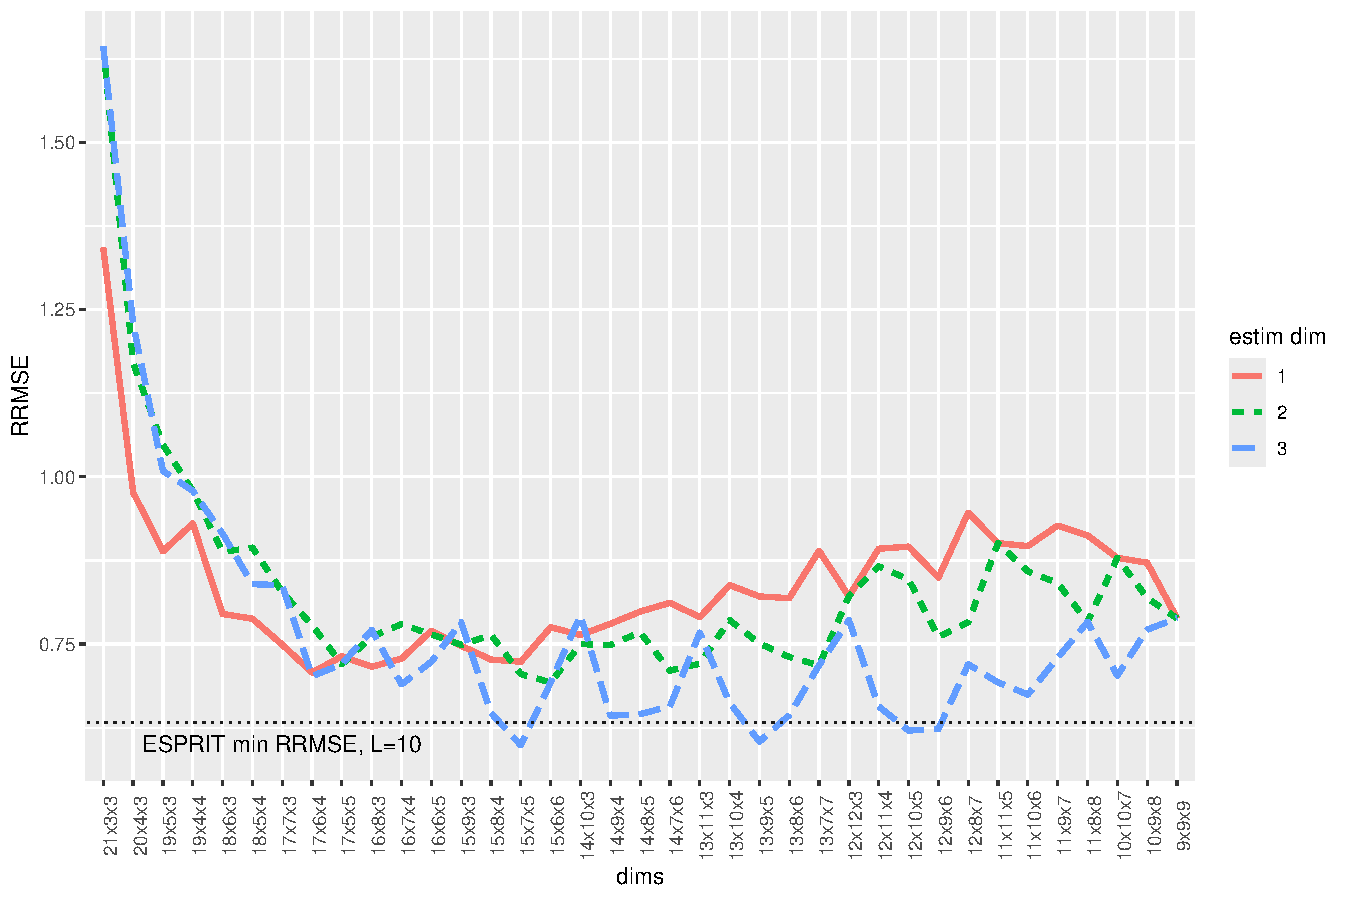
\includegraphics[width=\linewidth]{freq1_dims_no_rates.pdf}
    \caption{RRMSE оценок $\omega_1$.}
    \label{fig:freq1_dims_no_rates}
  \end{subfigure}
  \begin{subfigure}{0.49\linewidth}
    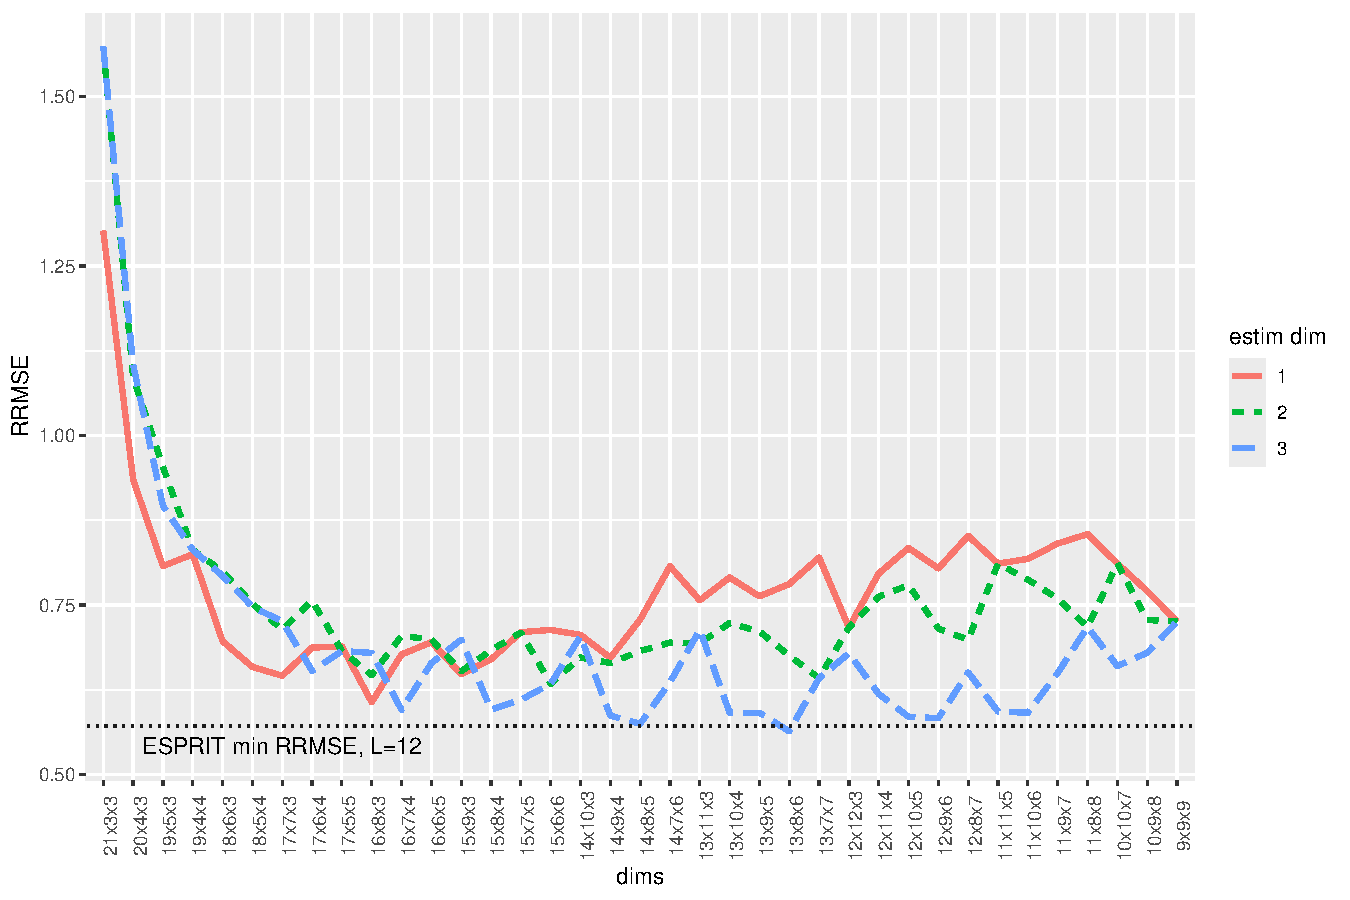
\includegraphics[width=\linewidth]{freq2_dims_no_rates.pdf}
    \caption{RRMSE оценок $\omega_2$.}
    \label{fig:freq2_dims_no_rates}
  \end{subfigure}
  \caption{Зависимость RRMSE оценок параметров одногомерного ряда
    от длины окна и направления усечения,
  случай~\ref{enum:esprit-no-rates}.}
  \label{fig:dims_no_rates}
\end{figure}
\begin{figure}[!ht]
  \centering
  \begin{subfigure}{0.49\linewidth}
    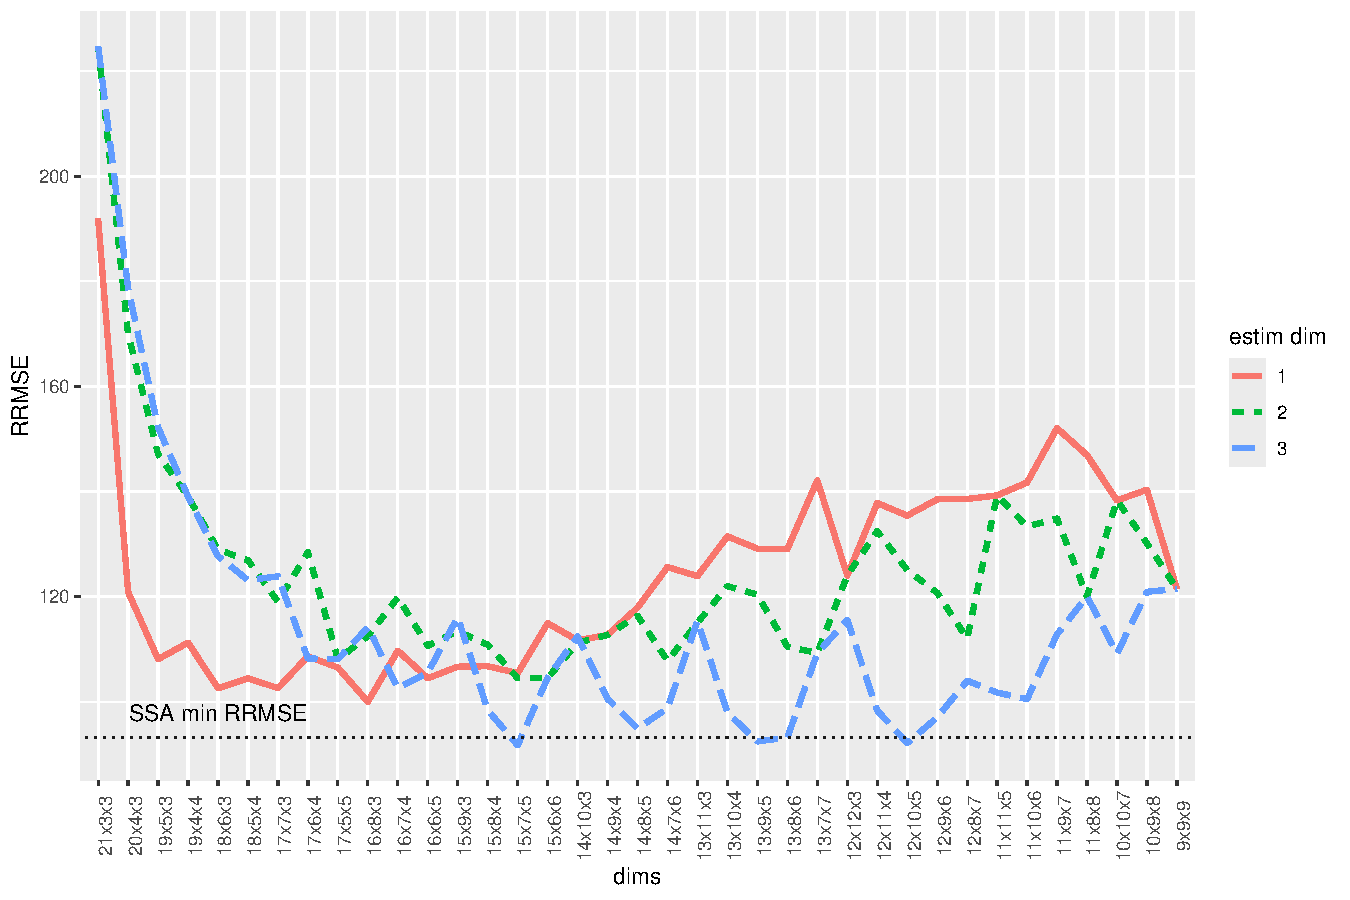
\includegraphics[width=\linewidth,
    height=0.167\textheight]{rate1_dims_small_eq_rates.pdf}
    \caption{RRMSE оценок $\alpha_1$.}
    \label{fig:rate1_dims_small_eq_rates}
  \end{subfigure}
  \begin{subfigure}{0.49\linewidth}
    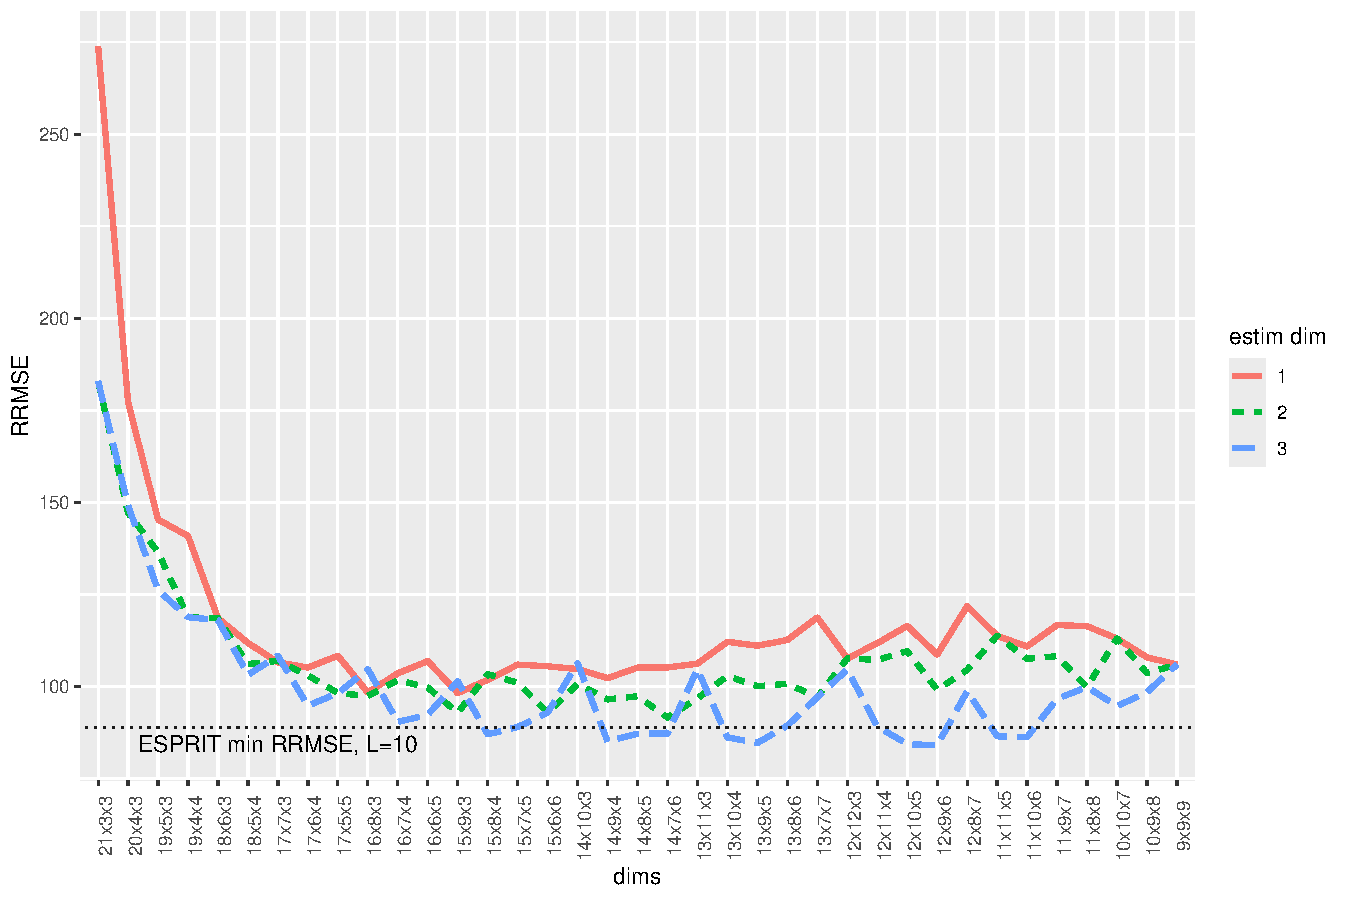
\includegraphics[width=\linewidth,
    height=0.167\textheight]{rate2_dims_small_eq_rates.pdf}
    \caption{RRMSE оценок $\alpha_2$.}
    \label{fig:rate2_dims_small_eq_rates}
  \end{subfigure}
  \begin{subfigure}{0.49\linewidth}
    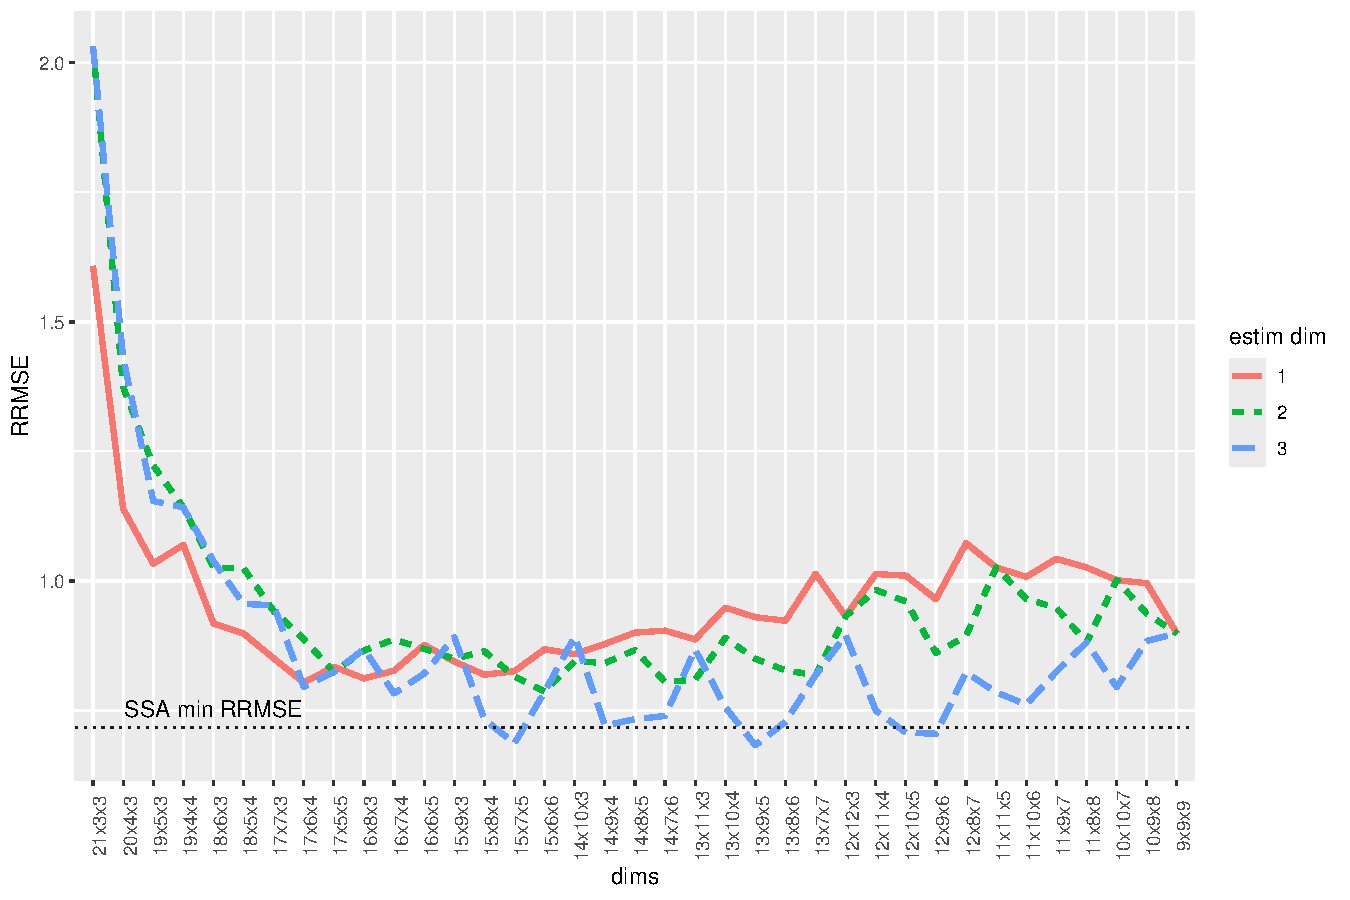
\includegraphics[width=\linewidth,
    height=0.167\textheight]{freq1_dims_small_eq_rates.pdf}
    \caption{RRMSE оценок $\omega_1$.}
    \label{fig:freq1_dims_small_eq_rates}
  \end{subfigure}
  \begin{subfigure}{0.49\linewidth}
    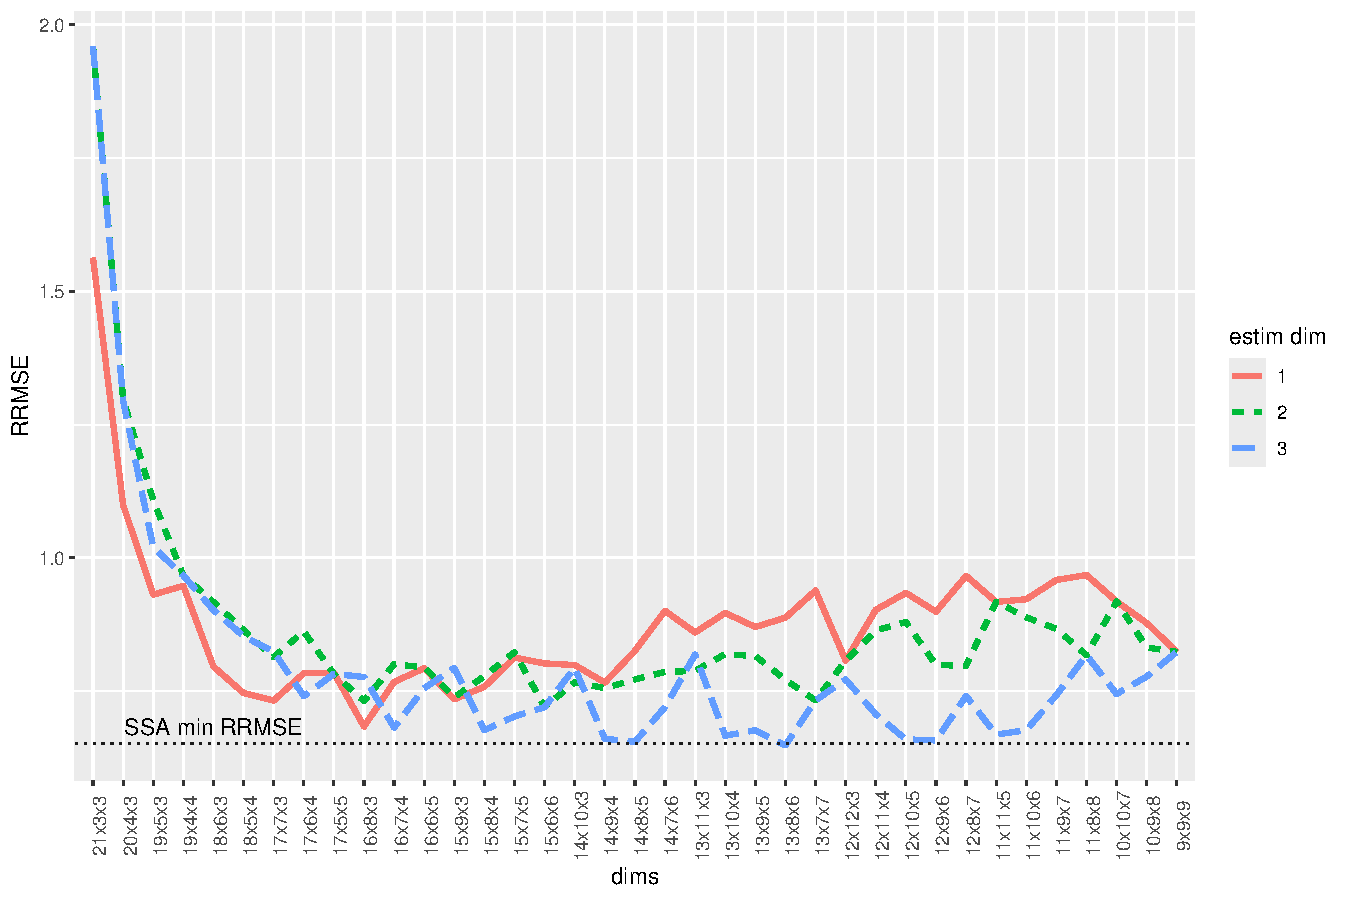
\includegraphics[width=\linewidth,
    height=0.167\textheight]{freq2_dims_small_eq_rates.pdf}
    \caption{RRMSE оценок $\omega_2$.}
    \label{fig:freq2_dims_small_eq_rates}
  \end{subfigure}
  \caption{Зависимость RRMSE оценок параметров одногомерного ряда
    от длины окна и направления усечения,
  случай~\ref{enum:esprit-smalleq-rates}.}
  \label{fig:dims_small_eq_rates}
\end{figure}
\begin{figure}[!ht]
  \centering
  \begin{subfigure}{0.49\linewidth}
    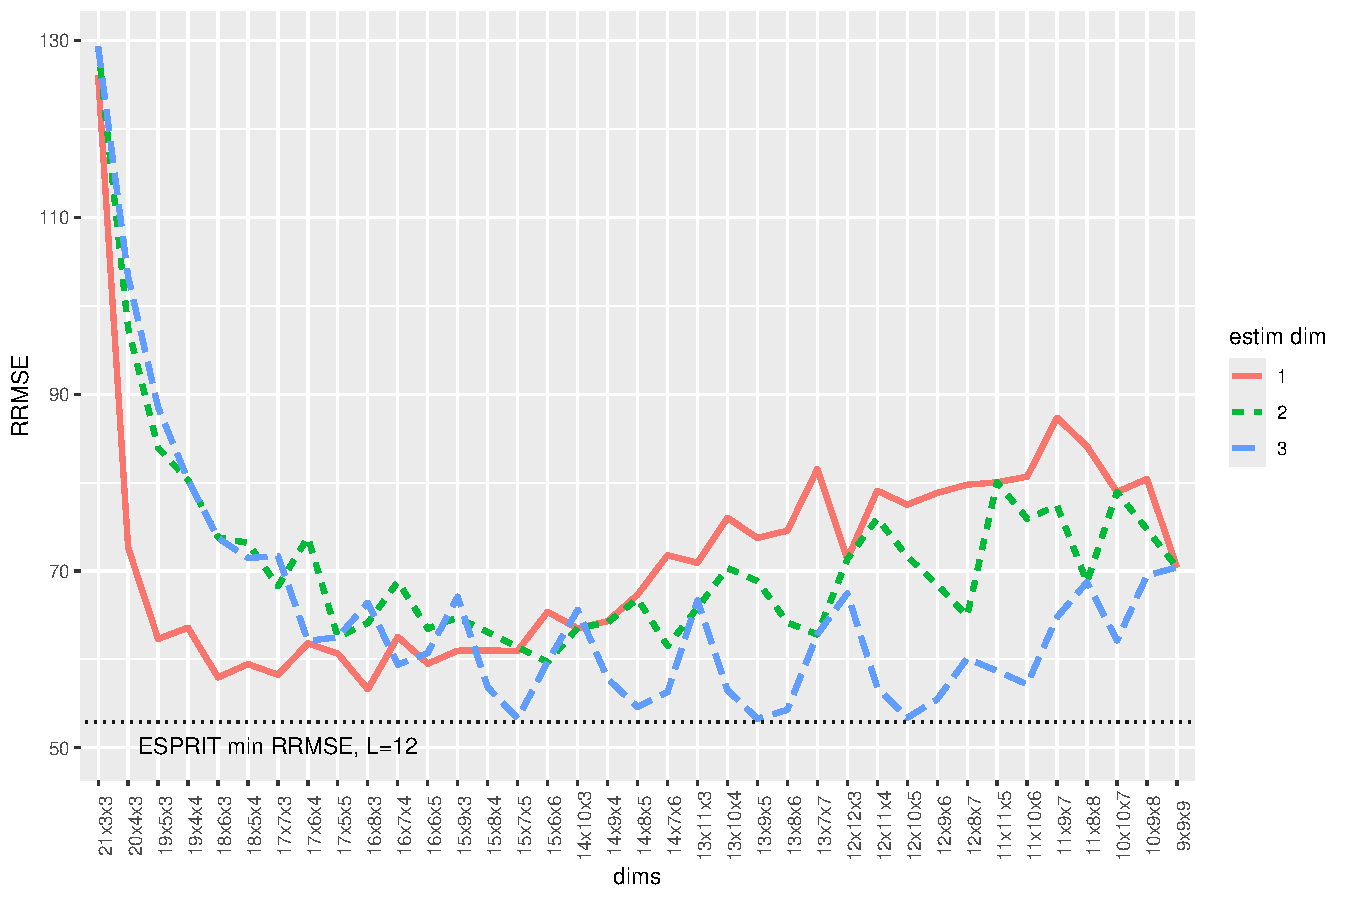
\includegraphics[width=\linewidth,
    height=0.167\textheight]{rate1_dims_large_eq_rates.pdf}
    \caption{RRMSE оценок $\alpha_1$.}
    \label{fig:rate1_dims_large_eq_rates}
  \end{subfigure}
  \begin{subfigure}{0.49\linewidth}
    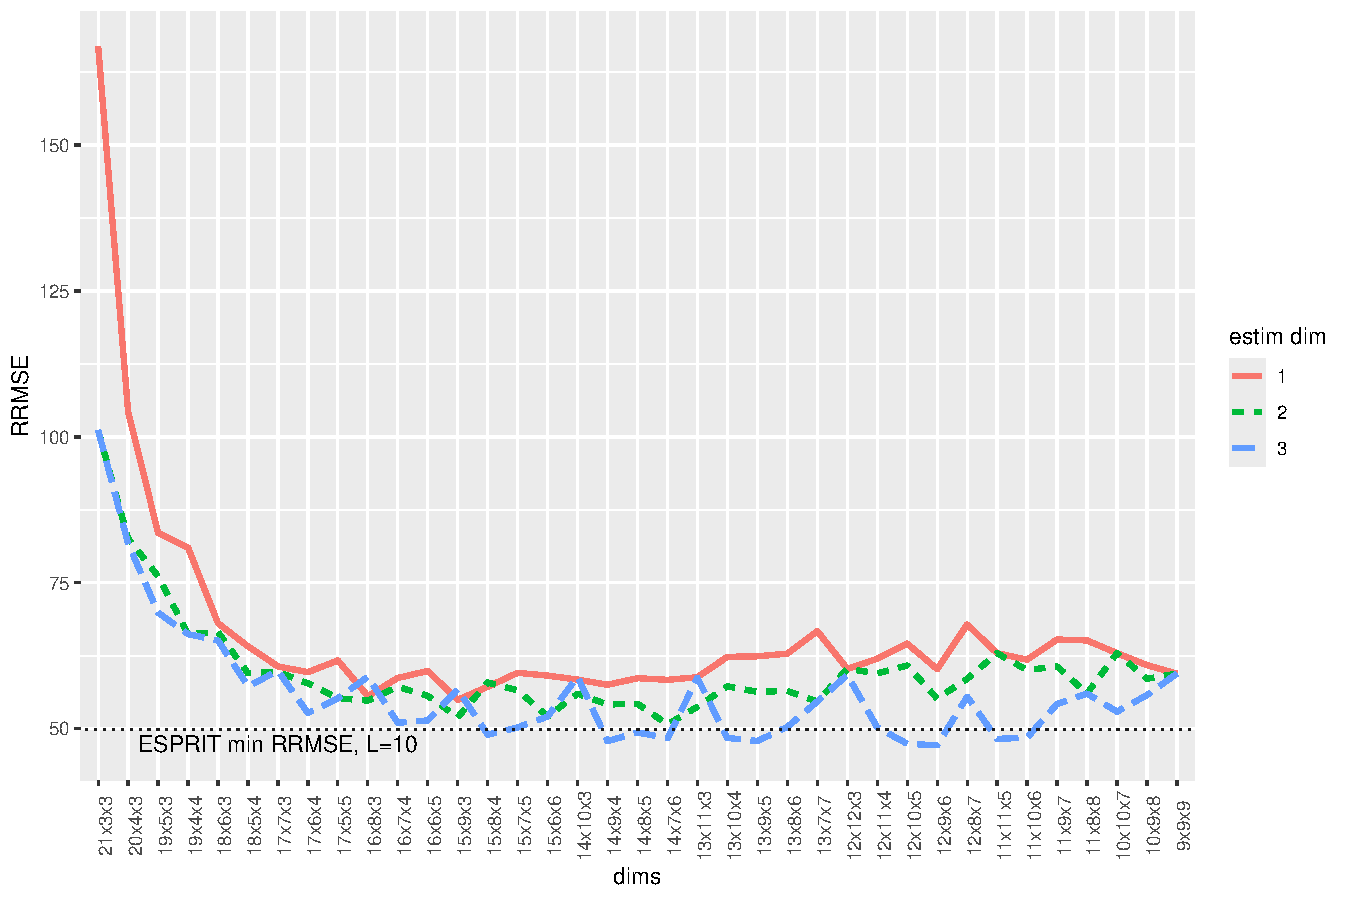
\includegraphics[width=\linewidth,
    height=0.167\textheight]{rate2_dims_large_eq_rates.pdf}
    \caption{RRMSE оценок $\alpha_2$.}
    \label{fig:rate2_dims_large_eq_rates}
  \end{subfigure}
  \begin{subfigure}{0.49\linewidth}
    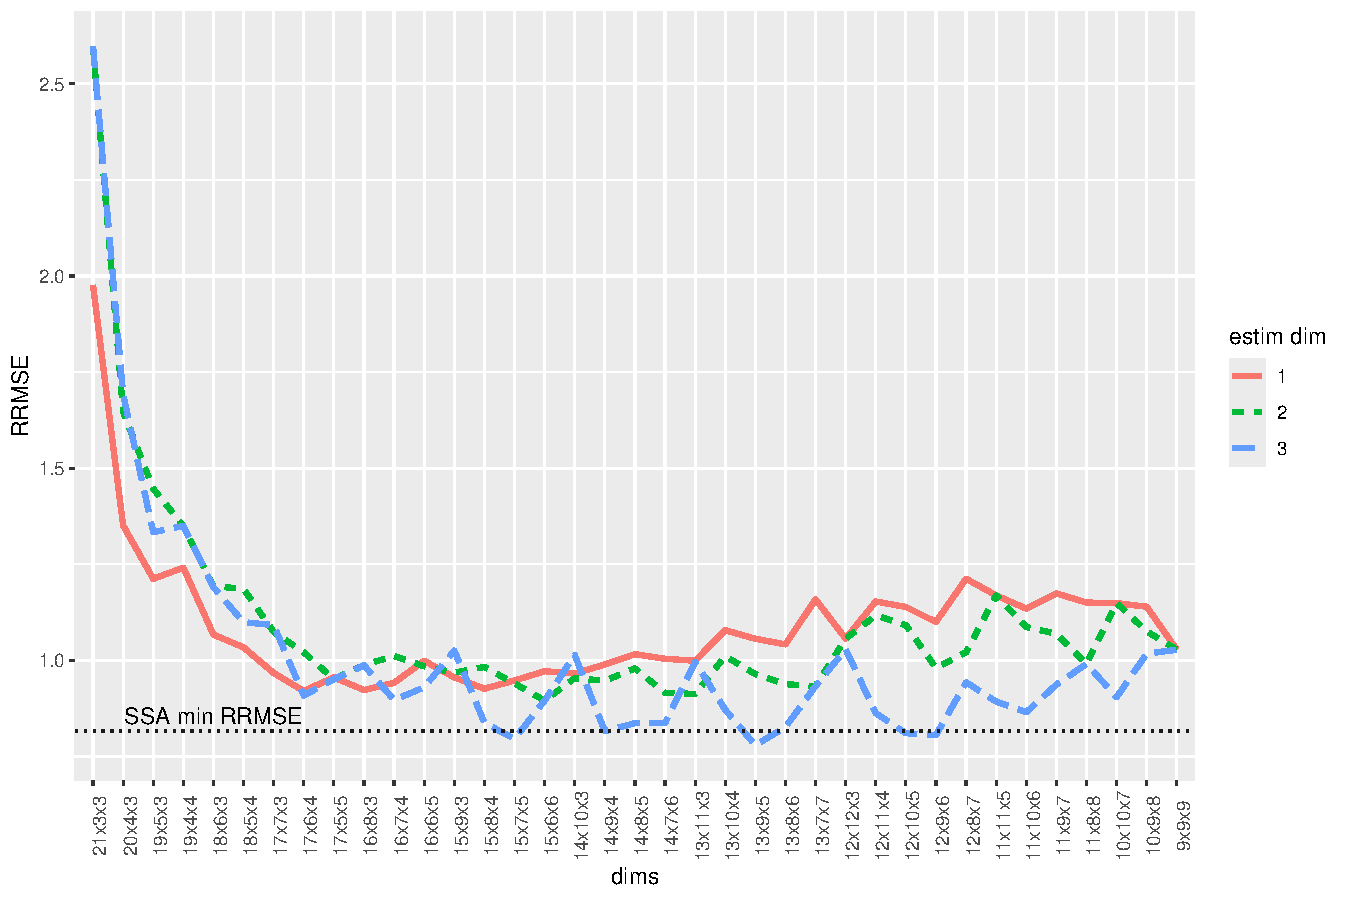
\includegraphics[width=\linewidth,
    height=0.167\textheight]{freq1_dims_large_eq_rates.pdf}
    \caption{RRMSE оценок $\omega_1$.}
    \label{fig:freq1_dims_large_eq_rates}
  \end{subfigure}
  \begin{subfigure}{0.49\linewidth}
    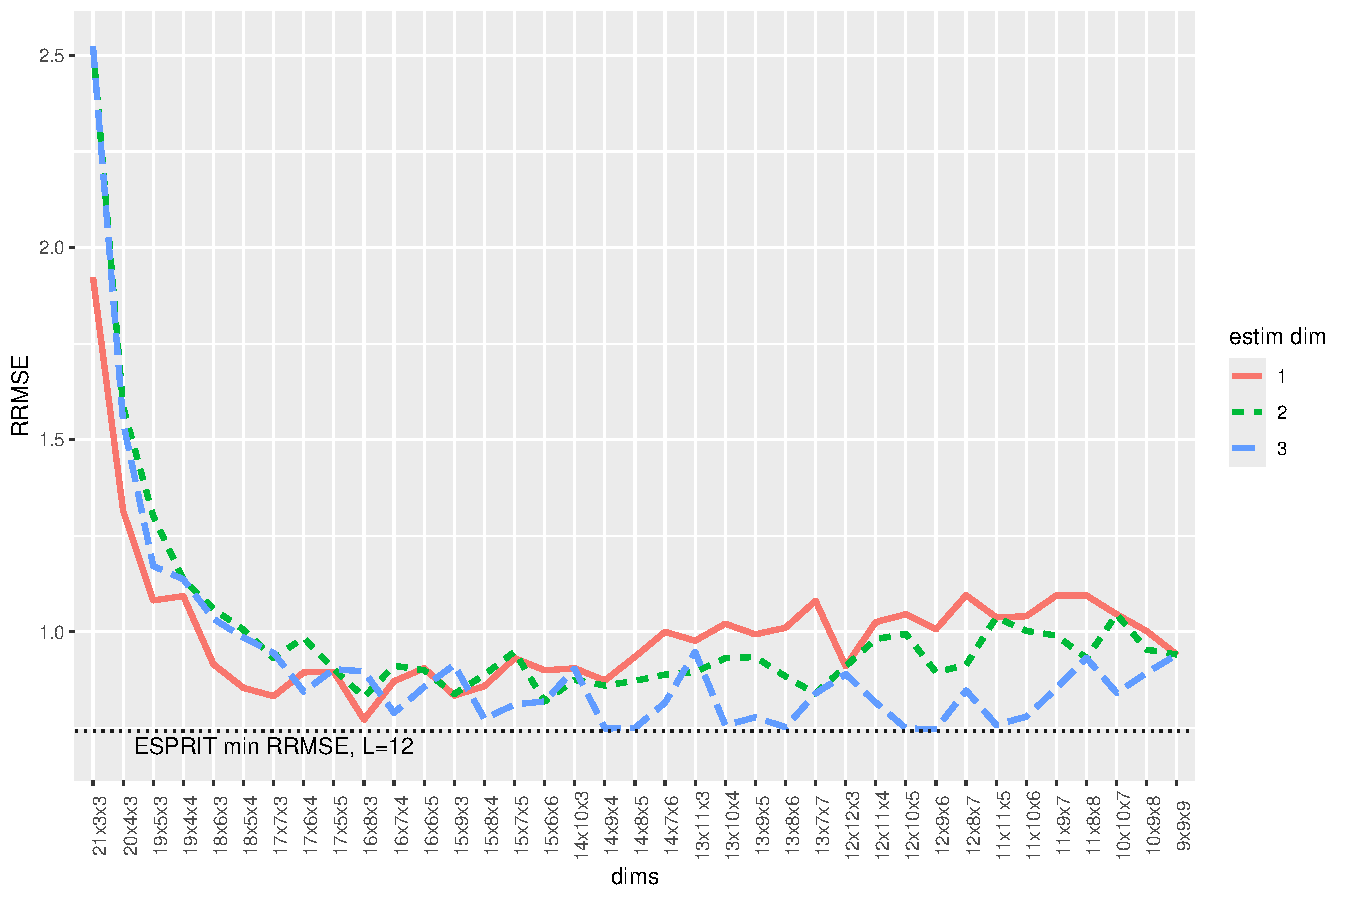
\includegraphics[width=\linewidth,
    height=0.167\textheight]{freq2_dims_large_eq_rates.pdf}
    \caption{RRMSE оценок $\omega_2$.}
    \label{fig:freq2_dims_large_eq_rates}
  \end{subfigure}
  \caption{Зависимость RRMSE оценок параметров одногомерного ряда
    от длины окна и направления усечения,
  случай~\ref{enum:esprit-bigeq-rates}.}
  \label{fig:dims_large_eq_rates}
\end{figure}
\begin{figure}[!ht]
  \centering
  \begin{subfigure}{0.49\linewidth}
    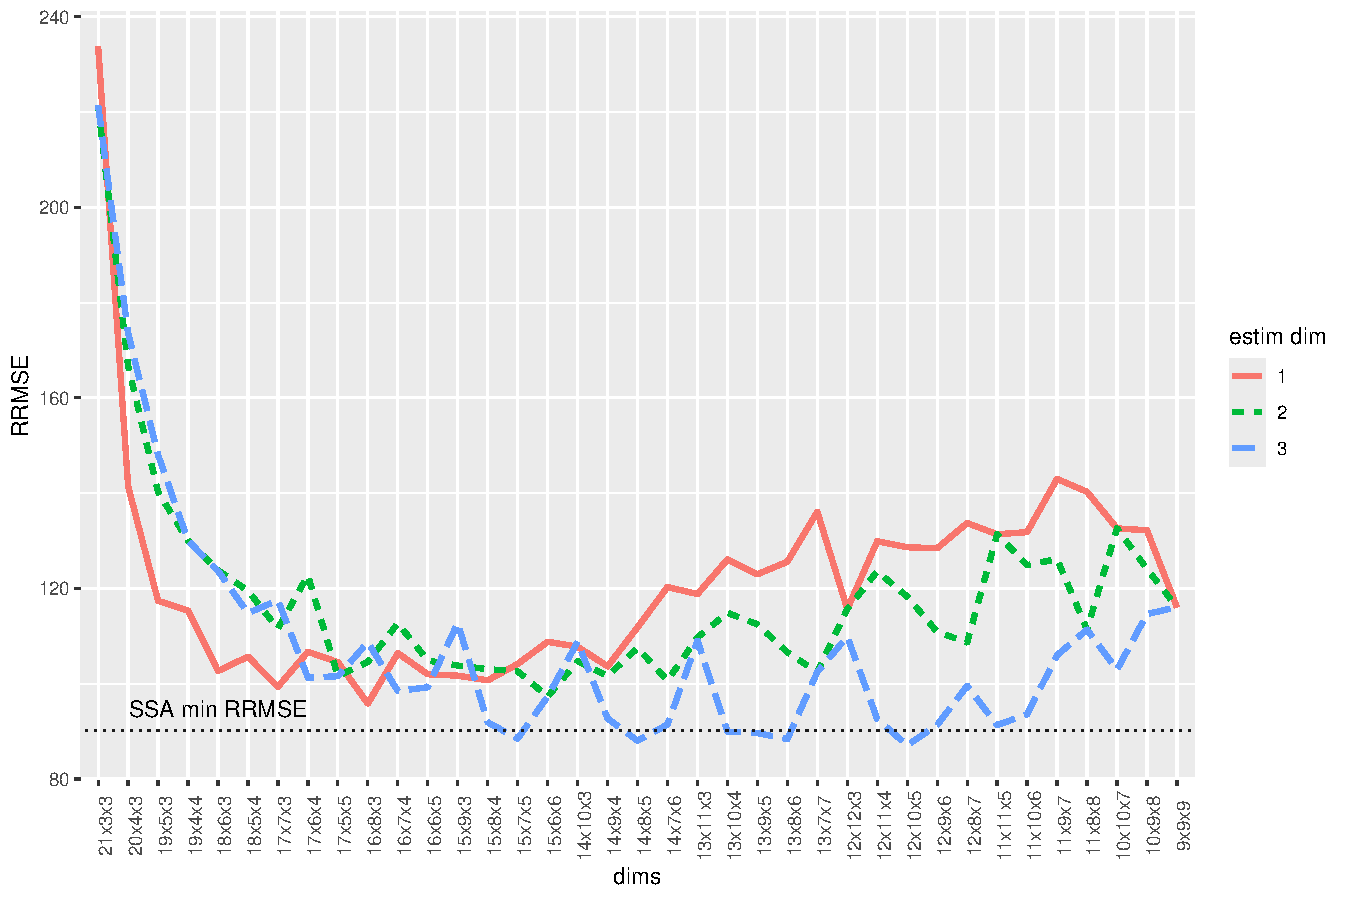
\includegraphics[width=\linewidth,
    height=0.167\textheight]{rate1_dims.pdf}
    \caption{RRMSE оценок $\alpha_1$.}
    \label{fig:rate1_dims}
  \end{subfigure}
  \begin{subfigure}{0.49\linewidth}
    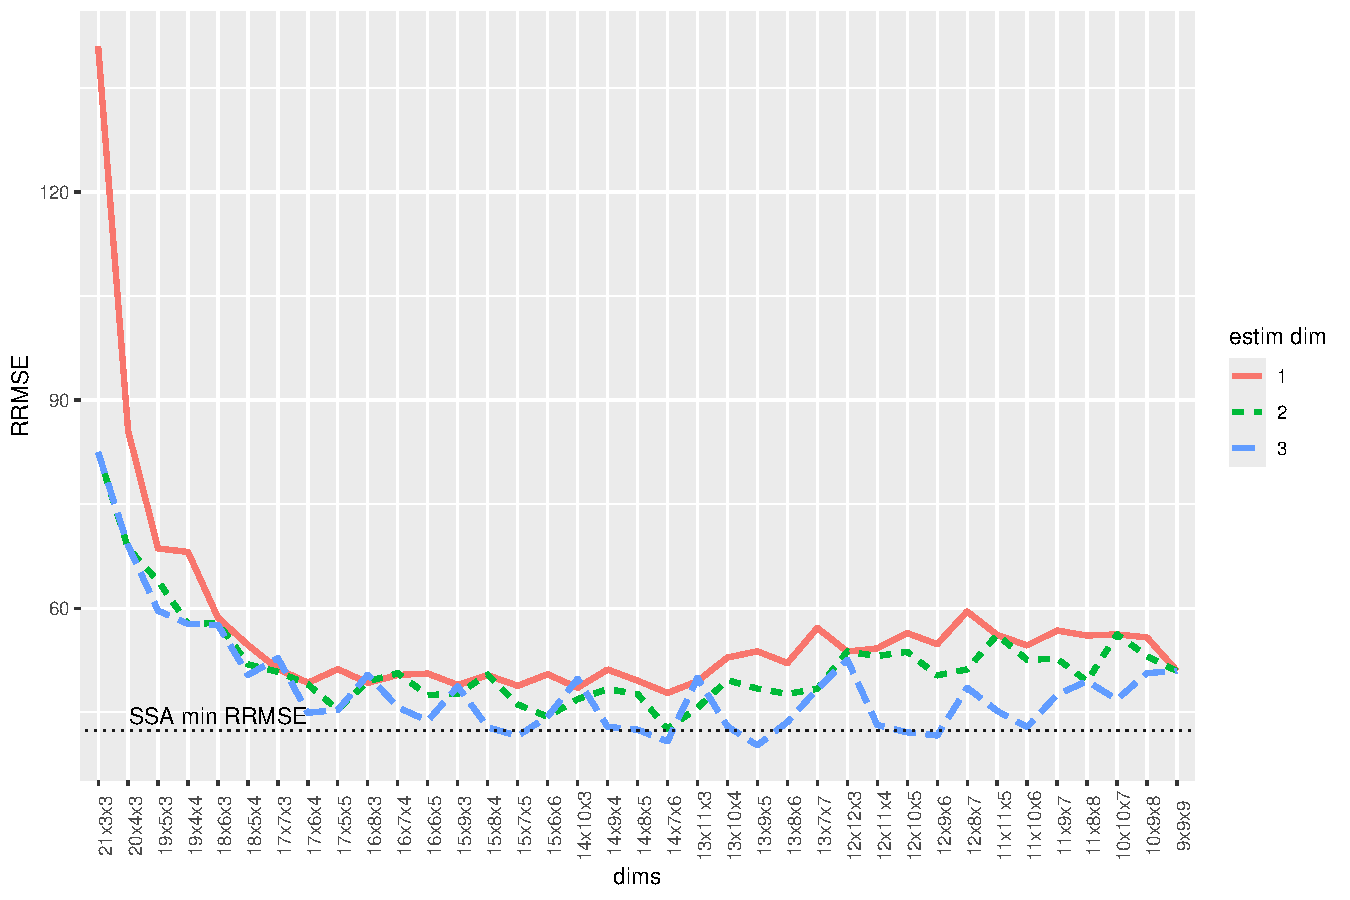
\includegraphics[width=\linewidth,
    height=0.167\textheight]{rate2_dims.pdf}
    \caption{RRMSE оценок $\alpha_2$.}
    \label{fig:rate2_dims}
  \end{subfigure}
  \begin{subfigure}{0.49\linewidth}
    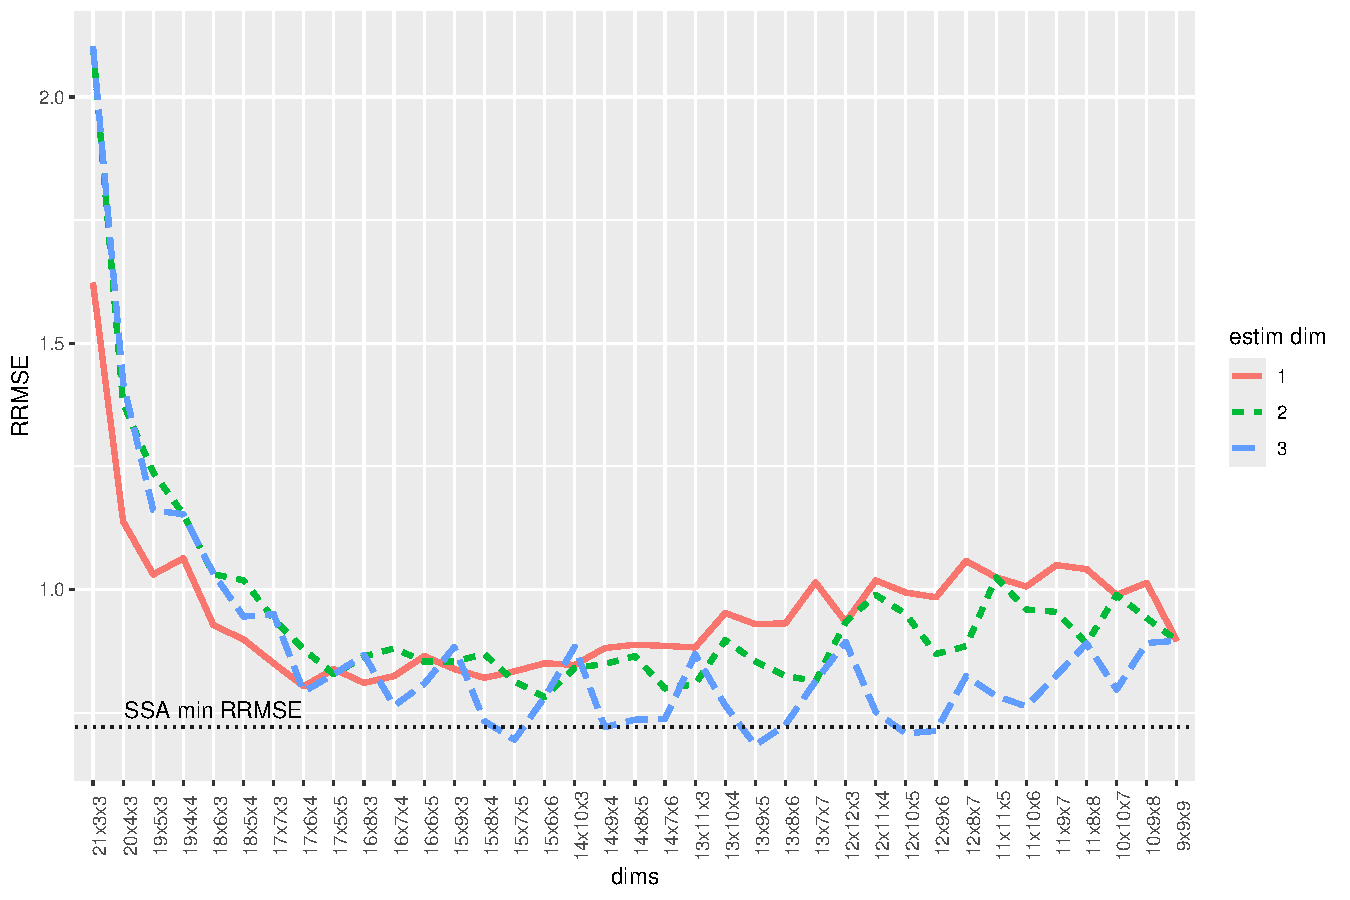
\includegraphics[width=\linewidth,
    height=0.167\textheight]{freq1_dims.pdf}
    \caption{RRMSE оценок $\omega_1$.}
    \label{fig:freq1_dims}
  \end{subfigure}
  \begin{subfigure}{0.49\linewidth}
    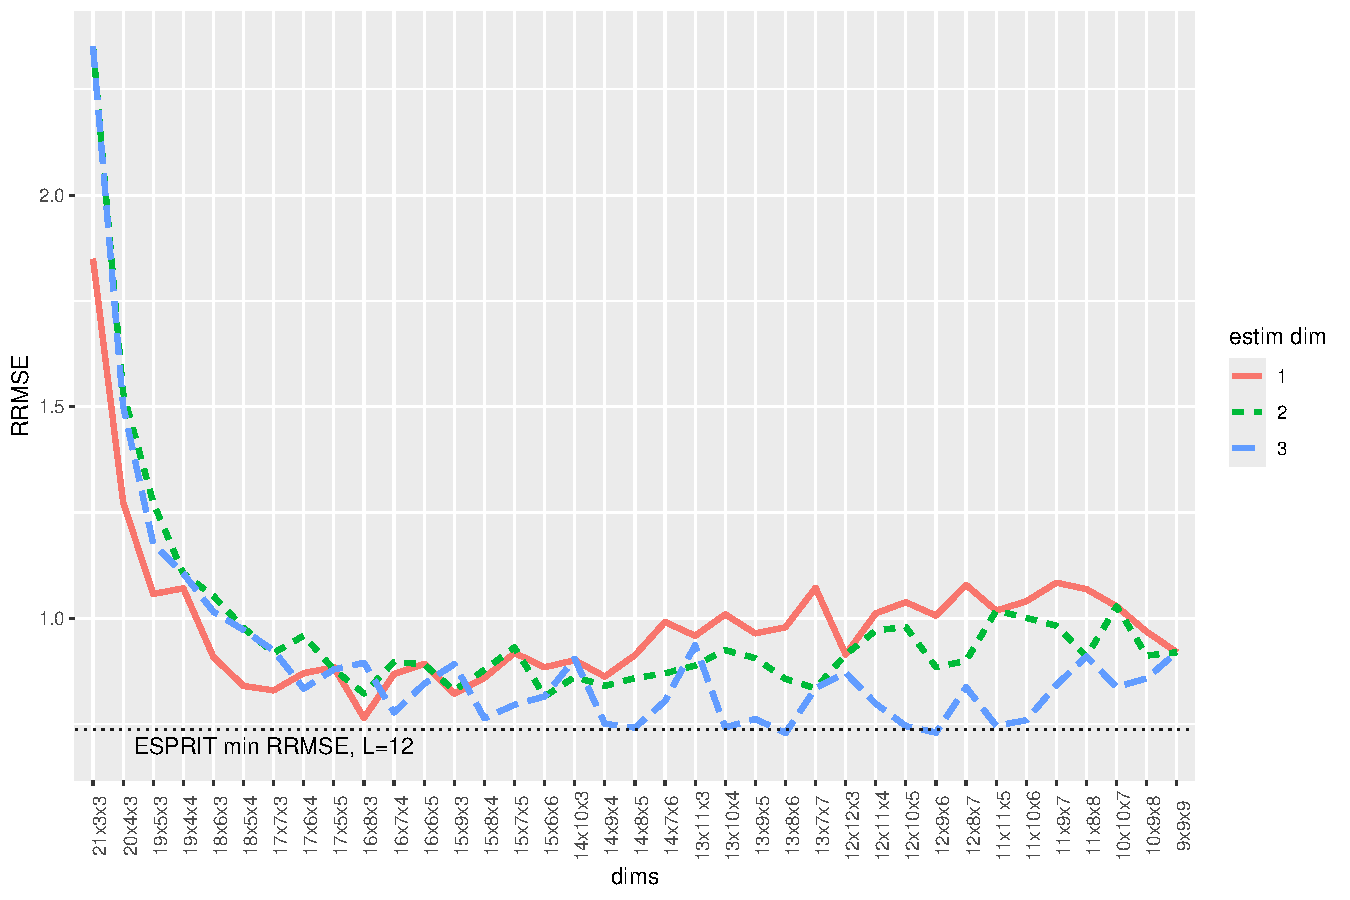
\includegraphics[width=\linewidth,
    height=0.167\textheight]{freq2_dims.pdf}
    \caption{RRMSE оценок $\omega_2$.}
    \label{fig:freq2_dims}
  \end{subfigure}
  \caption{Зависимость RRMSE оценок параметров одногомерного ряда
    от длины окна и направления усечения,
  случай~\ref{enum:esprit-diff-rates}.}
  \label{fig:dims_diff_rates}
\end{figure}

\paragraph{Выводы из численных сравнений}
В случае одномерных сигналов оценки методом HO-ESPRIT при оптимальном
подборе параметров
оказались не менее точными, чем оптимальные оценки стандартным методом ESPRIT.
Кроме того, в некоторых ситуациях оптимальные оценки методом
HO-ESPRIT оказываются точнее
оптимальных оценок методом ESPRIT.
Это соответствует результатам работы~\cite{hosvd-hooi-separation}, в
которой методы
сравнивались только при оптимальных размерах длины окна.
Однако множество длин окна в алгоритме HO-ESPRIT, при которых
точность оценок параметров сигнала
близка к оптимальной, очень мало, и нам пока неизвестны способы их
выбора кроме перебора.
С другой стороны, для стандартного алгоритма ESPRIT требуется меньший
набор параметров,
а разница между методами в точности оценки при оптимальных
параметрах невелика.
В связи с этим, использование метода HO-ESPRIT для
оценки параметров одномерных сигналов в
текущем виде не обосновано.

Стоит заметить, что во всех случаях выбор номера направления $d$ из
алгоритма~\ref{alg:ho-esprit}, соответствующего направлению
наименьшего размера
траекторного тензора, давал наиболее точные результаты.

\subsection{Многомерный случай}\label{subsec:mv-esprit-comparison}
Пусть $M=12$ и $R=2$, то есть многомерный временной ряд
\begin{gather*}
  \tX = \left(\tX^{(1)}, \tX^{(2)}, \ldots, \tX^{(12)}\right),\\
  \tX^{(m)} = \left(x_1^{(m)}, x_2^{(m)}, \ldots, x_{25}^{(m)}\right)
\end{gather*}
состоит из элементов вида
\[
  x_{n + 1}^{(m)} = a_1^{(m)} e^{ \alpha_1 n }
  e^{2 \pi \iu \omega_1 n} +
  a_2^{(m)} e^{ \alpha_2 n }
  e^{2 \pi \iu \omega_2 n} + \zeta_n^{(m)},
\]
где $n \in \overline{0:24}$, а $\zeta_n^{(m)}$ "--- независимые
случайные величины из
распределения $\mathrm{CN}(0,\, \sigma^2)$, $\sigma=0.2$.
Значения частот и варианты степеней затухания были взяты такими же, как
в одномерном случае в разделе~\ref{subsec:esprit-comparison}.
В качестве амплитуд $a_k^{(m)}$ были взяты независимые реализации
случайных величин из распределения $\mathrm{CN}(0,\, 1)$,
их приблизительные значения приведены в
выражении~\eqref{eq:complex-amplitudes}.
\begin{gather}
  \label{eq:complex-amplitudes}
  \begin{split}
    \operatorname{Re}(a_1) \approx \left( 0, -0.1, -1, -0.4, 0.2,
    0.3, -0.9, -0.3, -1.2, -0.2, 0.8, 0.5\right)^{\rmT}, \\
    \operatorname{Im}(a_1) \approx \left(-0.9, -0.3, -0.5, -0.6,
    -0.1, -0.2, -1.3, -0.1, 0.7, 0.1, -1, -1 \right)^{\rmT}, \\
    \operatorname{Re}(a_2) \approx \left( -0.2, 0.7, 0.5, 0.1, -0.7,
    -0.1, 0.7, 0.3, -0.4, -1.5, -0.5, -1.5\right)^{\rmT}, \\
    \operatorname{Im}(a_2) \approx \left( 0.3, -1.2, -0.2, -0.5, 0.8,
    -0.5, -0.6, 0.6, -0.7, 0, 0.2, -0.2\right)^{\rmT}. \\
  \end{split}
\end{gather}
Как и в одномерном случае, ранг сигналов с каждым набором параметров равен 2,
поэтому для оценки параметров использовались только первые два
сингулярных вектора разложения из алгоритмов~\ref{alg:esprit}
и~\ref{alg:ho-esprit}.
В качестве способа разложения траекторного тензора был выбран метод HOOI.

Ниже представлены графики зависимости RRMSE оценок параметров,
полученных методами M-ESPRIT и HO-M-ESPRIT, от значения длины окна $L$.

Рисунки~\ref{fig:L_no_rates} соответствуют случаю~\ref{enum:esprit-no-rates}.
Графики с RRMSE оценок степеней затухания не приводятся в этом
случае, так как для них RRMSE не определено.
Рисунки~\ref{fig:L_small_eq_rates},~\ref{fig:L_large_eq_rates}
и~\ref{fig:L_diff_rates}
соответствуют
случаям~\ref{enum:esprit-smalleq-rates},~\ref{enum:esprit-bigeq-rates}
и~\ref{enum:esprit-diff-rates}
соответственно.
\begin{figure}[!ht]
  \centering
  \begin{subfigure}{0.49\linewidth}
    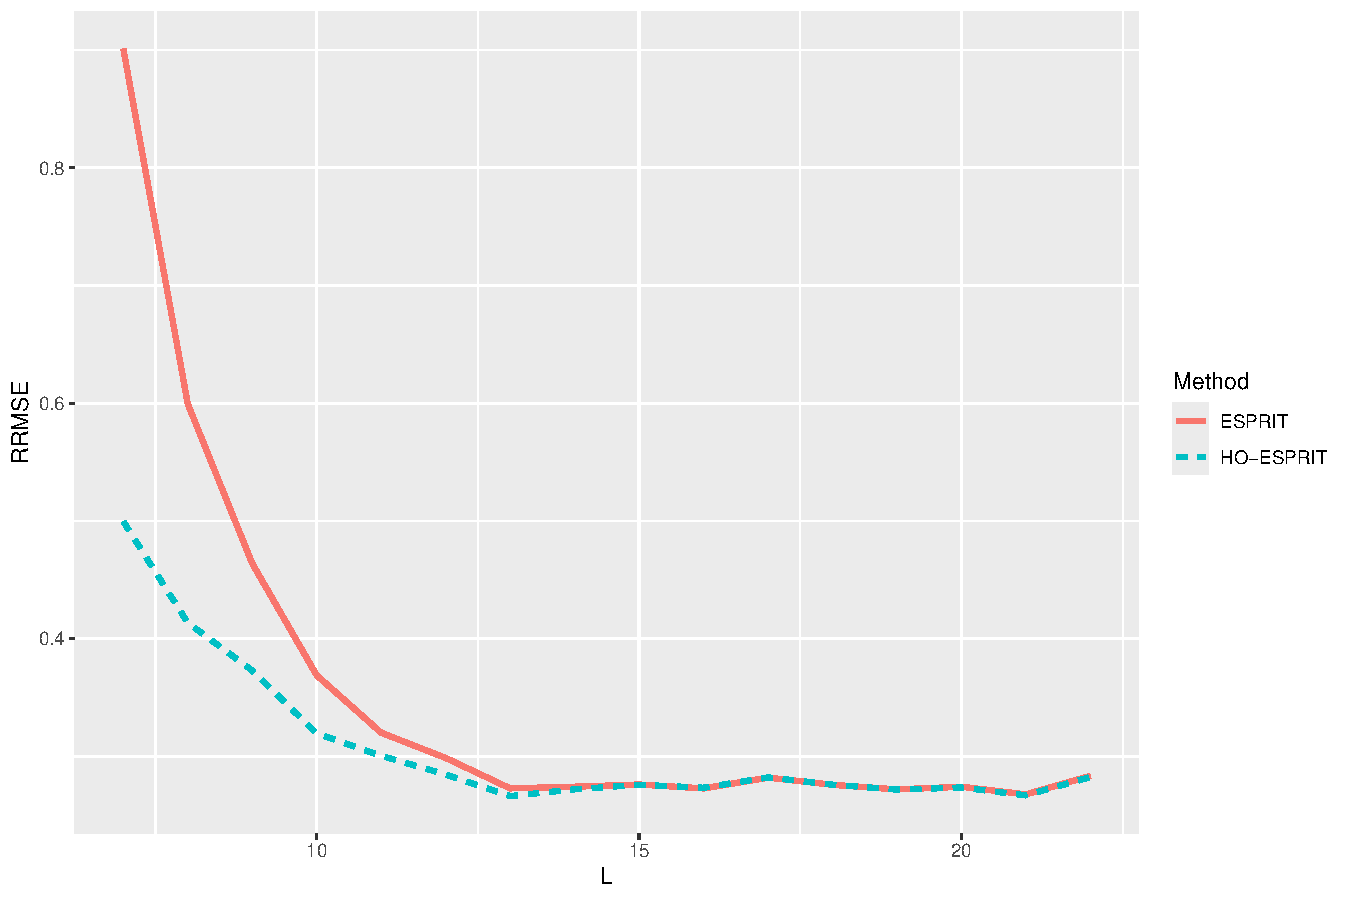
\includegraphics[width=\linewidth]{freq1_L_no_rates.pdf}
    \caption{RRMSE оценок $\omega_1$.}
    \label{fig:freq1_L_no_rates}
  \end{subfigure}
  \begin{subfigure}{0.49\linewidth}
    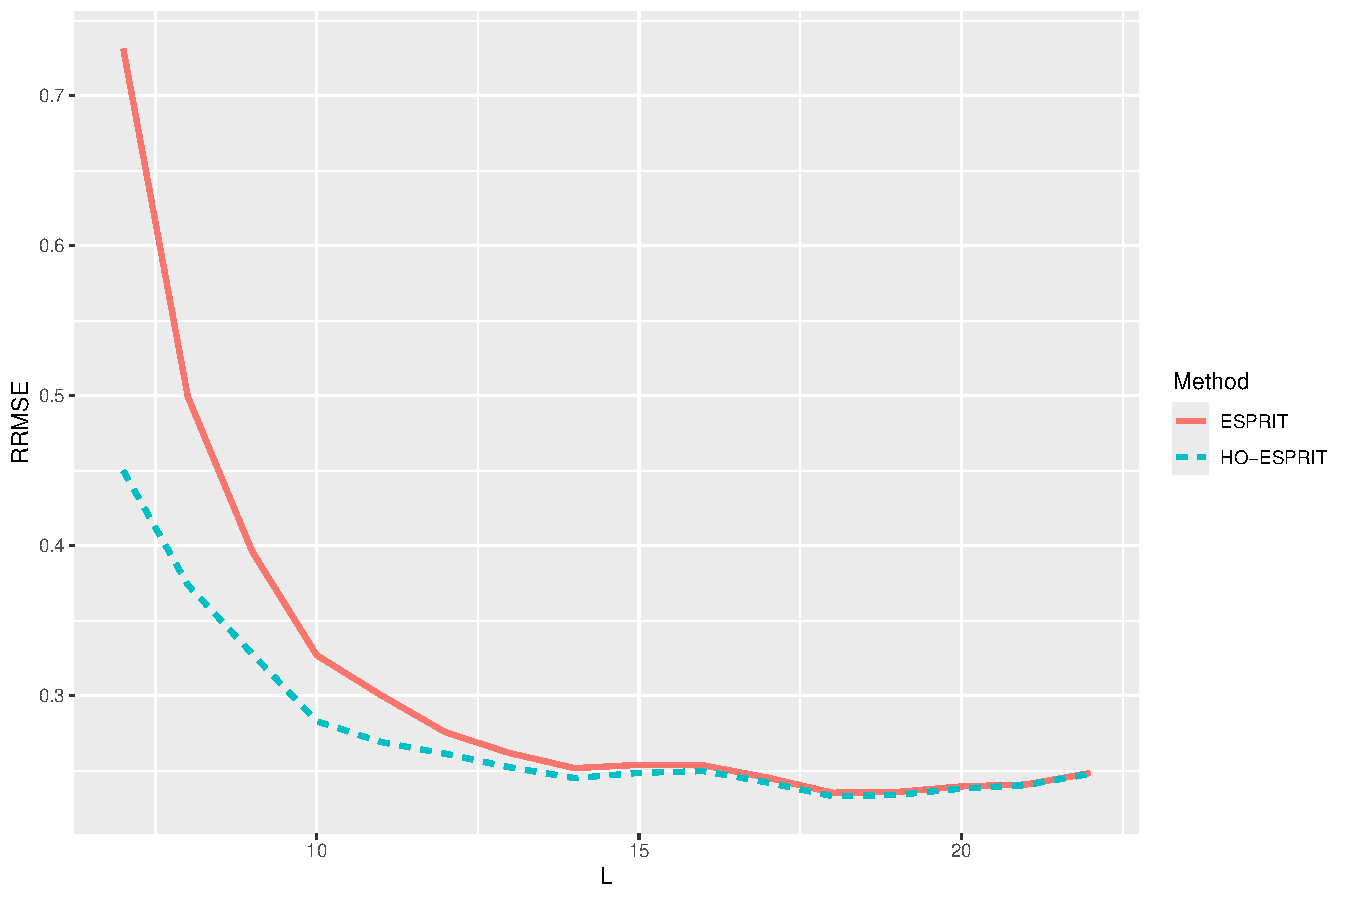
\includegraphics[width=\linewidth]{freq2_L_no_rates.pdf}
    \caption{RRMSE оценок $\omega_2$.}
    \label{fig:freq2_L_no_rates}
  \end{subfigure}
  \caption{Зависимость RRMSE оценок параметров многомерного ряда от
    длины окна,
  случай~\ref{enum:esprit-no-rates}.}
  \label{fig:L_no_rates}
\end{figure}

\begin{figure}[!ht]
  \centering
  \begin{subfigure}{0.49\linewidth}
    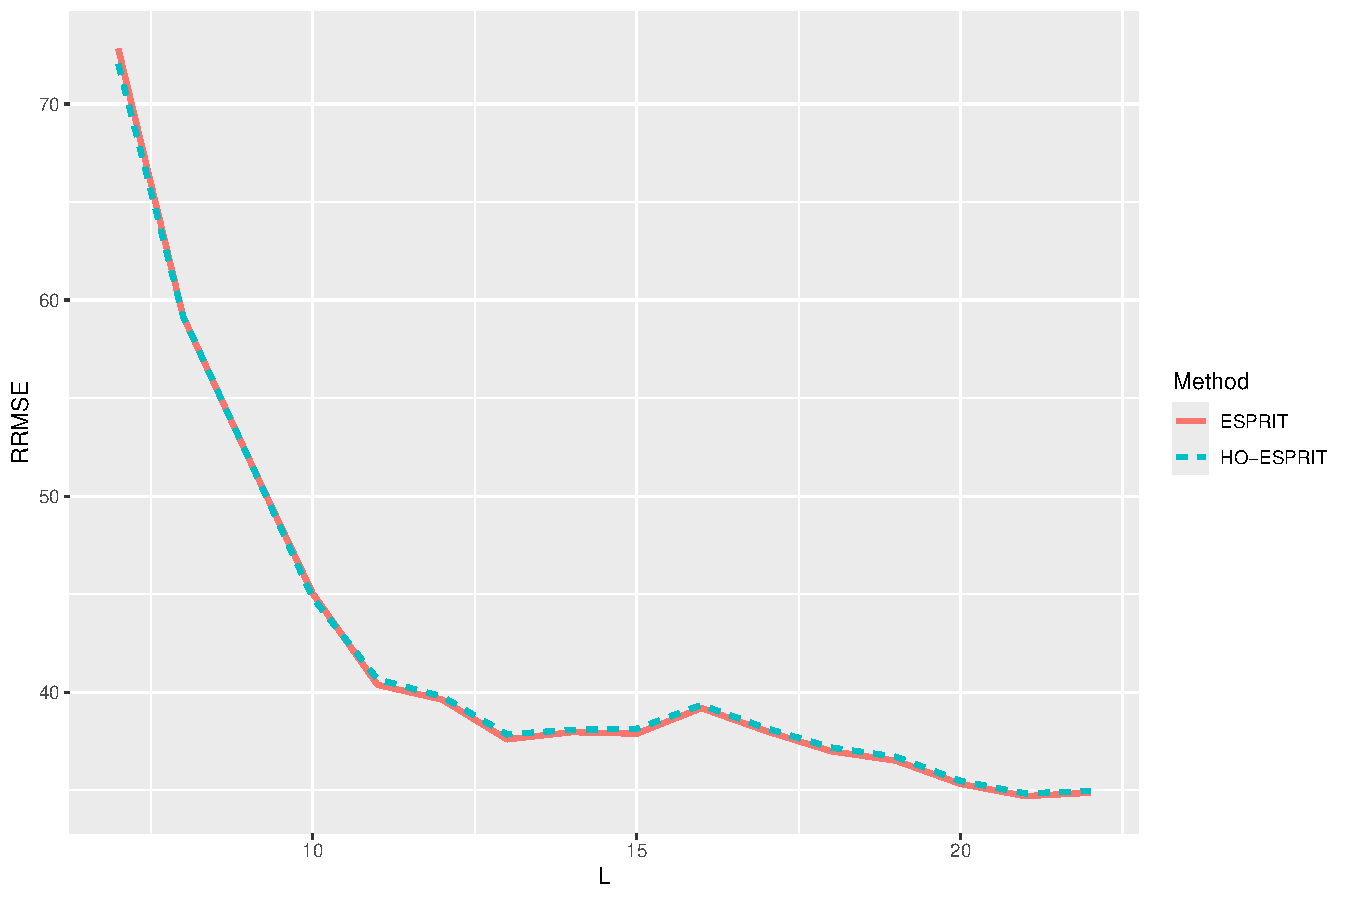
\includegraphics[width=\linewidth,
    height=0.19\textheight]{rate1_L_small_eq_rates.pdf}
    \caption{RRMSE оценок $\alpha_1$.}
    \label{fig:rate1_L_small_eq_rates}
  \end{subfigure}
  \begin{subfigure}{0.49\linewidth}
    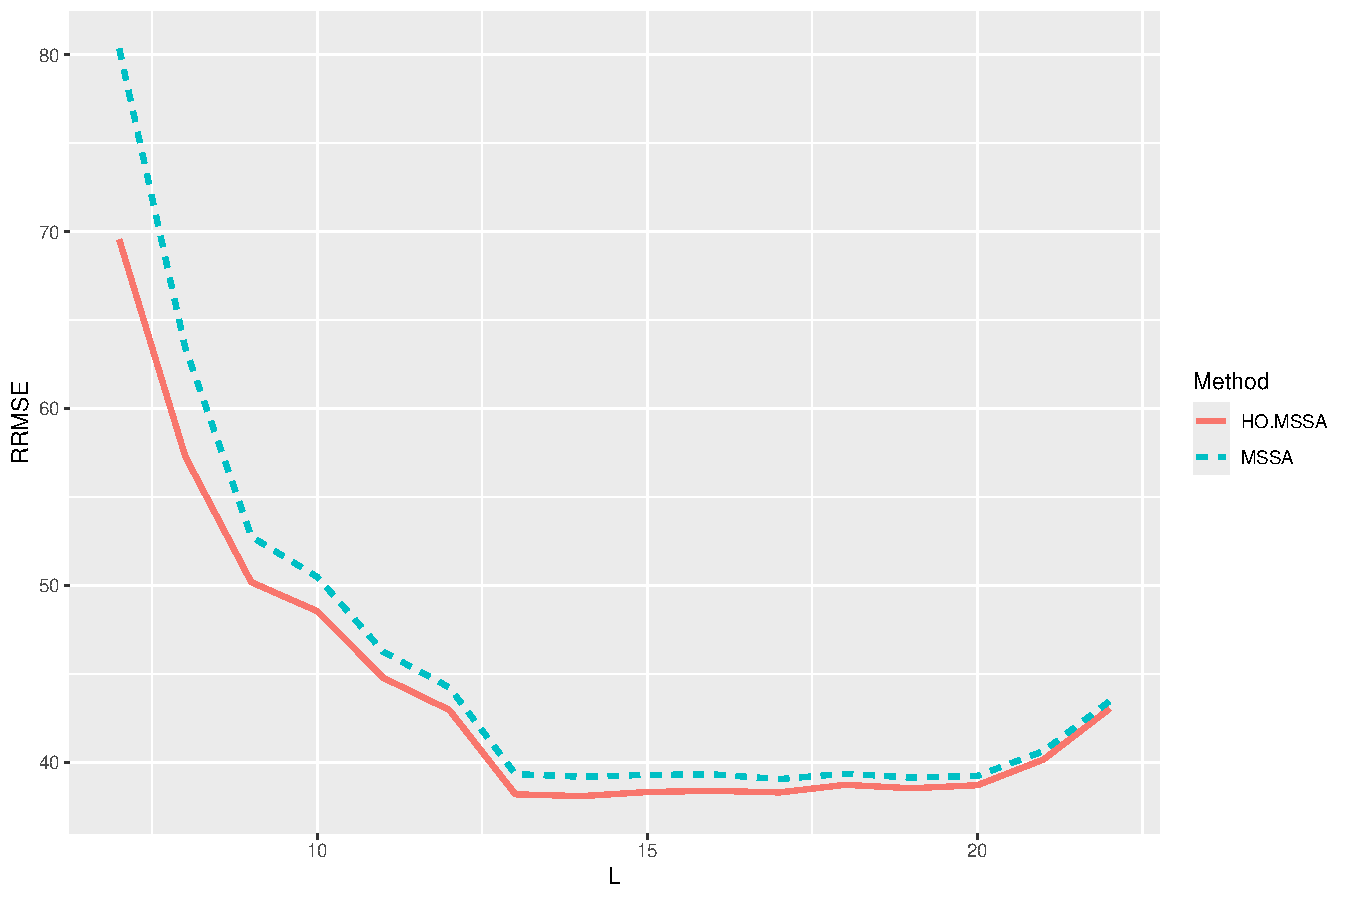
\includegraphics[width=\linewidth,
    height=0.19\textheight]{rate2_L_small_eq_rates.pdf}
    \caption{RRMSE оценок $\alpha_2$.}
    \label{fig:rate2_L_small_eq_rates}
  \end{subfigure}
  \begin{subfigure}{0.49\linewidth}
    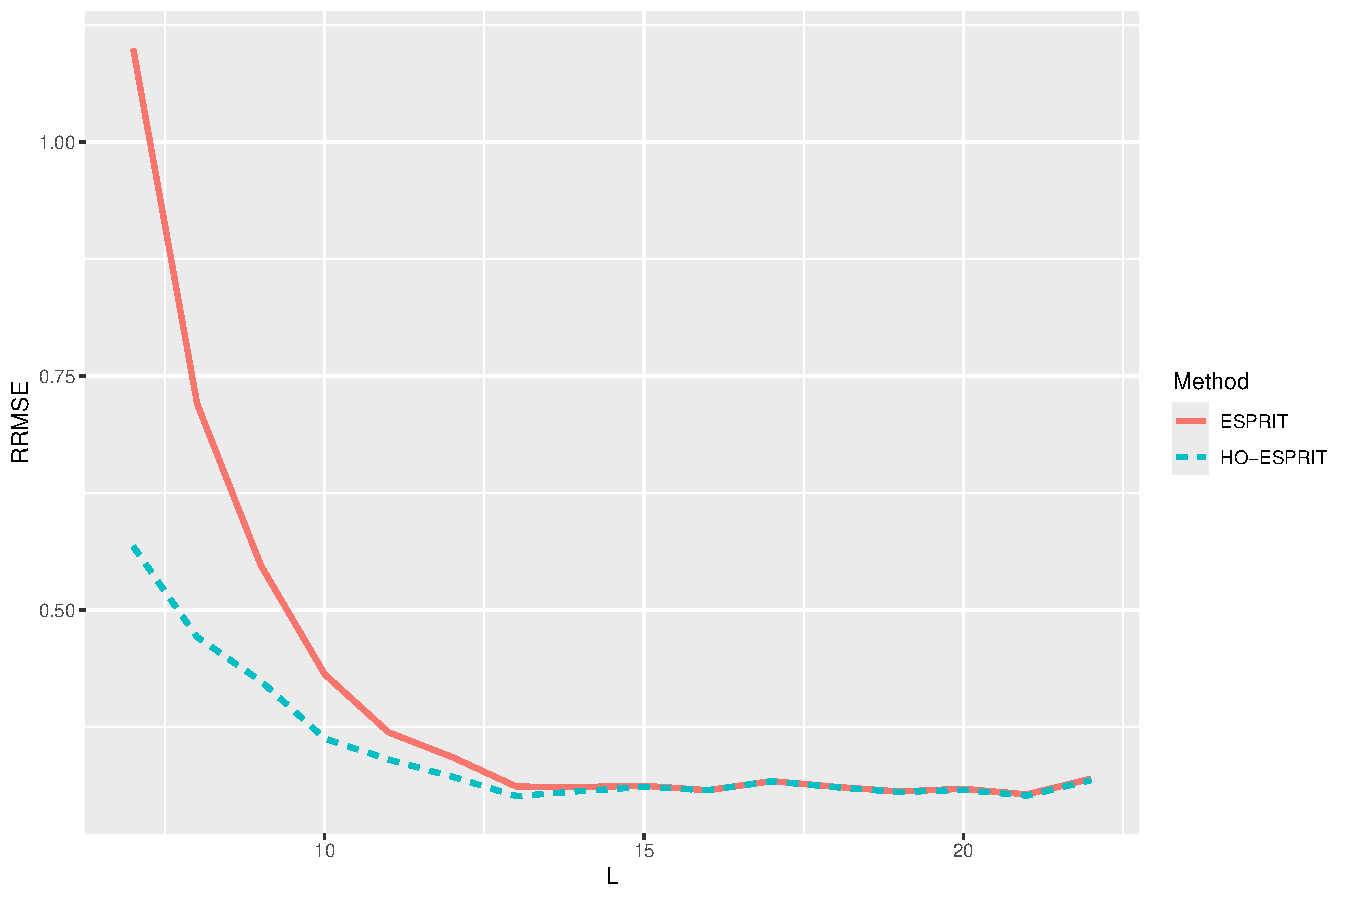
\includegraphics[width=\linewidth,
    height=0.19\textheight]{freq1_L_small_eq_rates.pdf}
    \caption{RRMSE оценок $\omega_1$.}
    \label{fig:freq1_L_small_eq_rates}
  \end{subfigure}
  \begin{subfigure}{0.49\linewidth}
    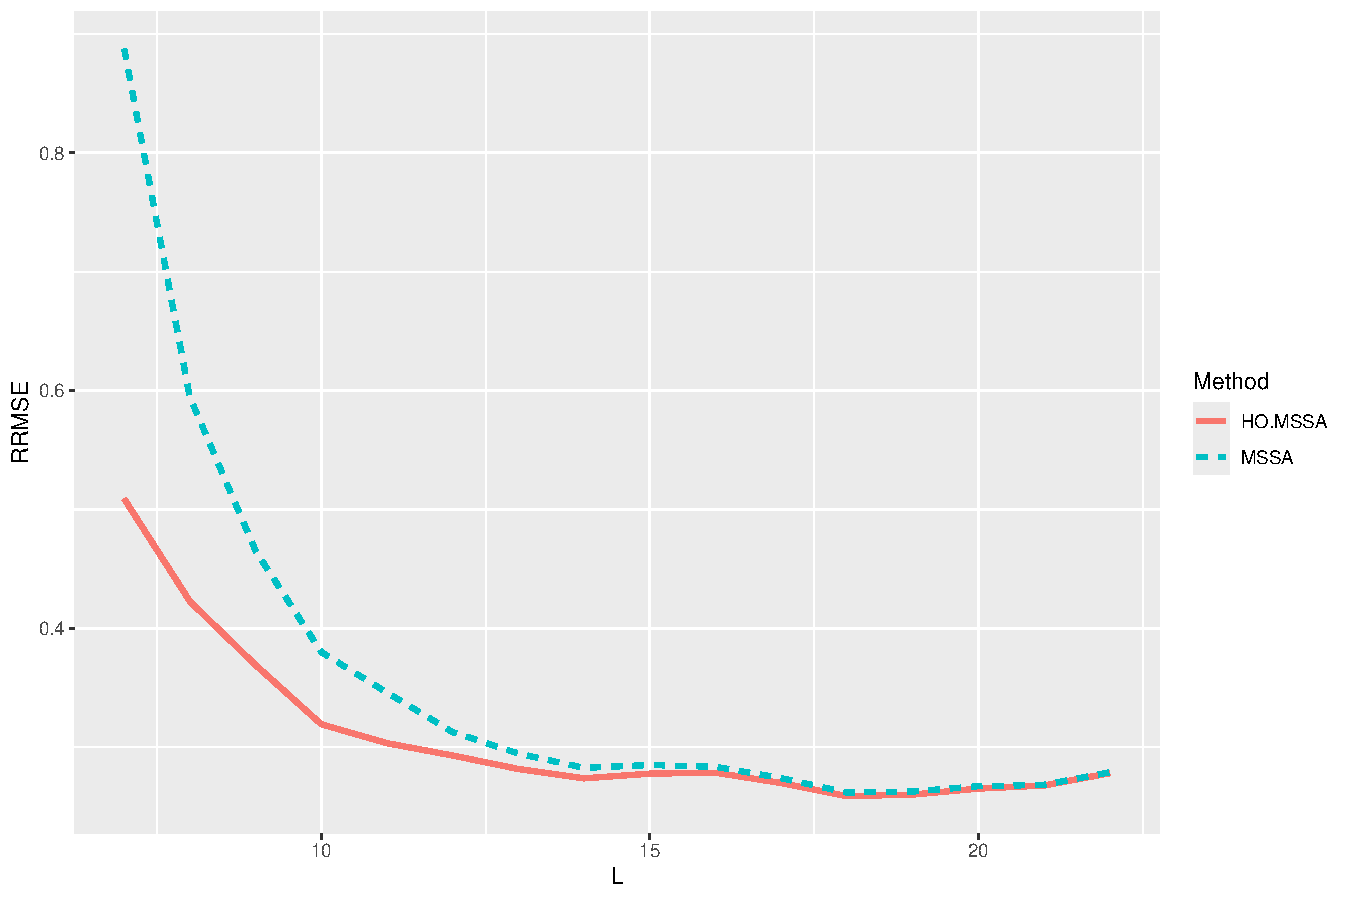
\includegraphics[width=\linewidth,
    height=0.19\textheight]{freq2_L_small_eq_rates.pdf}
    \caption{RRMSE оценок $\omega_2$.}
    \label{fig:freq2_L_small_eq_rates}
  \end{subfigure}
  \caption{Зависимость RRMSE оценок параметров многомерного ряда от
    длины окна,
  случай~\ref{enum:esprit-smalleq-rates}.}
  \label{fig:L_small_eq_rates}
\end{figure}

\begin{figure}[!ht]
  \centering
  \begin{subfigure}{0.49\linewidth}
    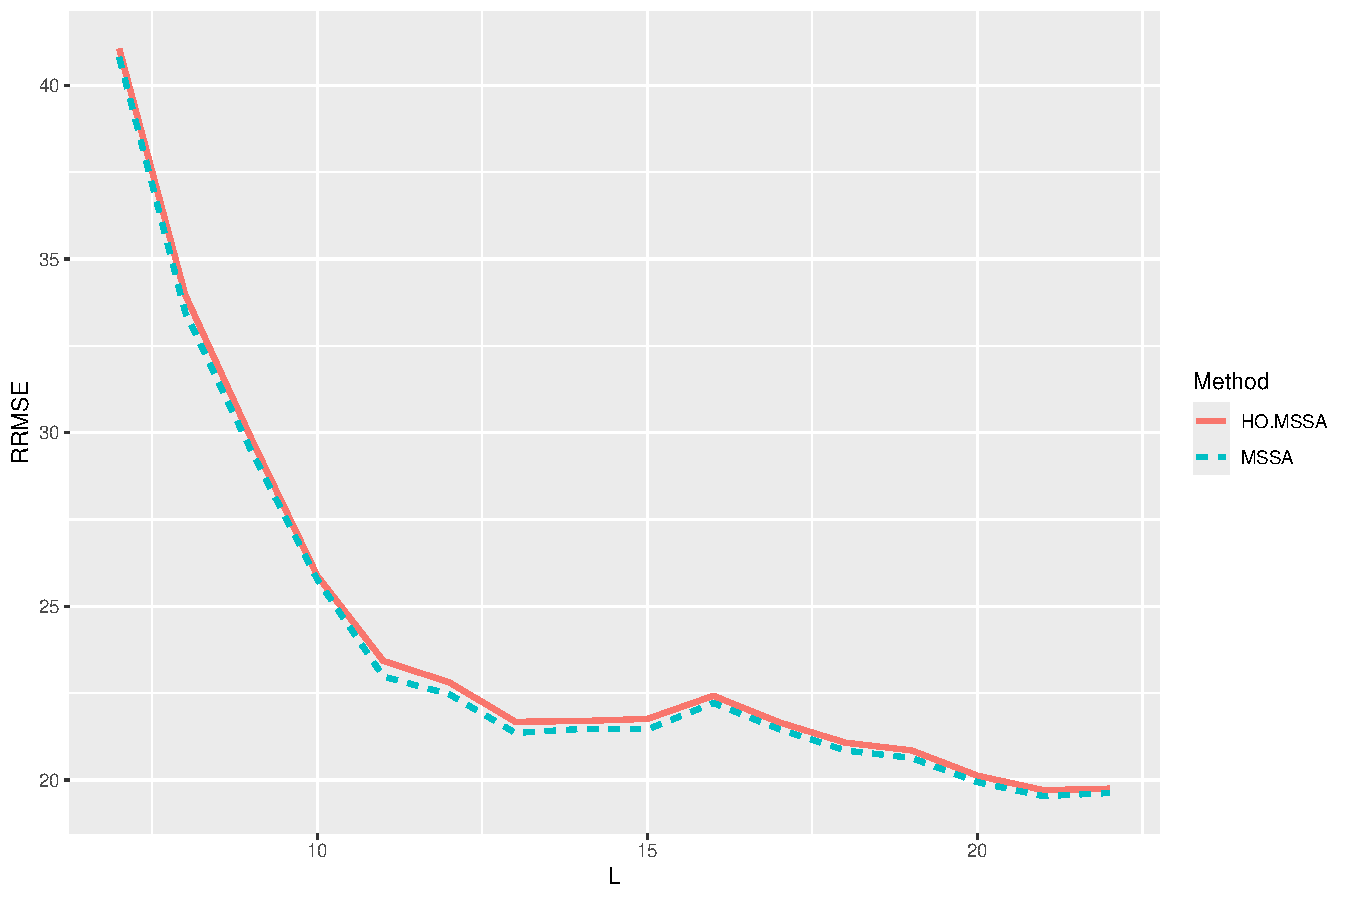
\includegraphics[width=\linewidth,
    height=0.167\textheight]{rate1_L_large_eq_rates.pdf}
    \caption{RRMSE оценок $\alpha_1$.}
    \label{fig:rate1_L_large_eq_rates}
  \end{subfigure}
  \begin{subfigure}{0.49\linewidth}
    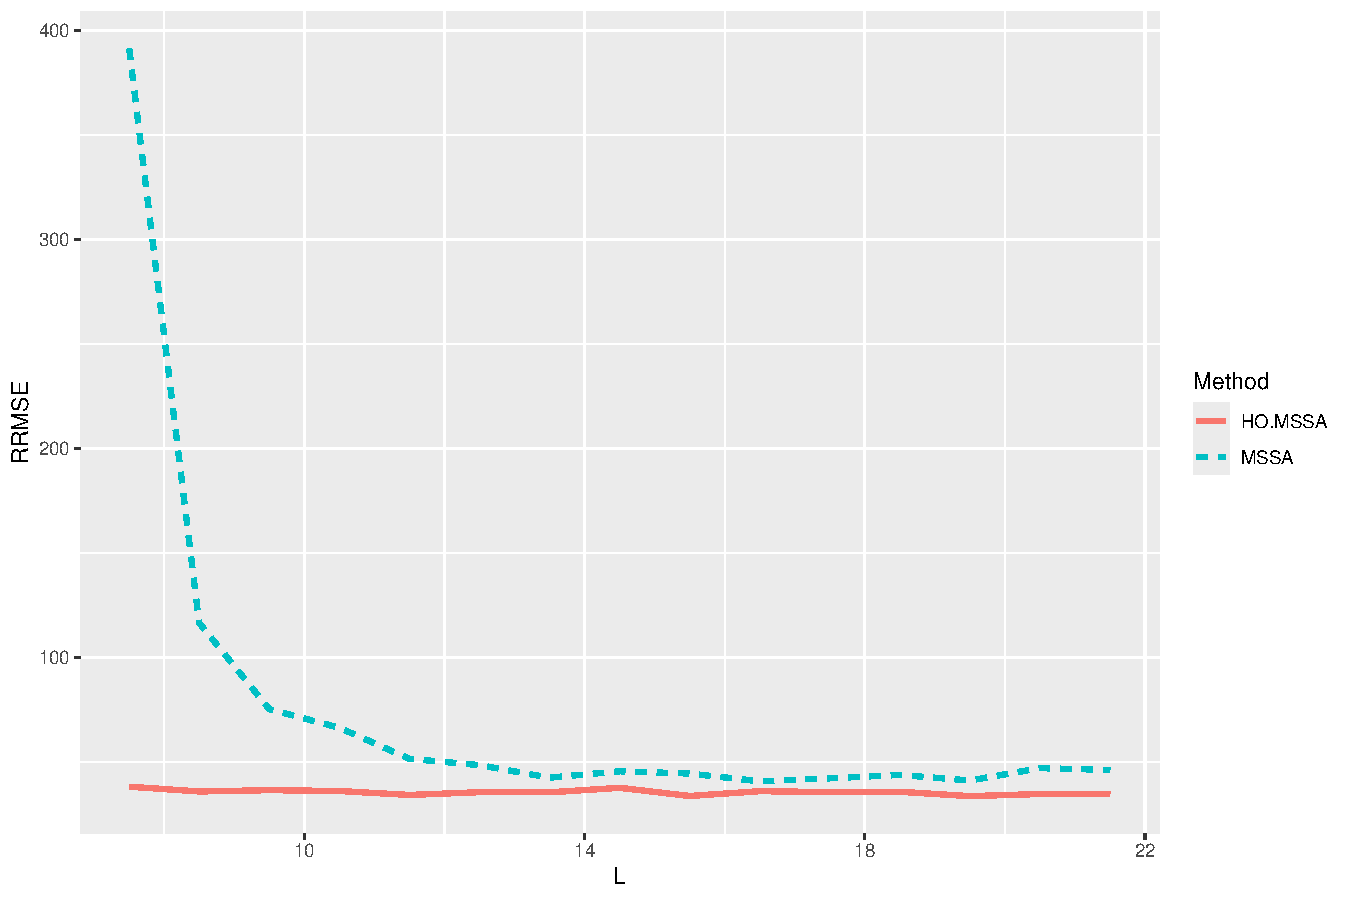
\includegraphics[width=\linewidth,
    height=0.167\textheight]{rate2_L_large_eq_rates.pdf}
    \caption{RRMSE оценок $\alpha_2$.}
    \label{fig:rate2_L_large_eq_rates}
  \end{subfigure}
  \begin{subfigure}{0.49\linewidth}
    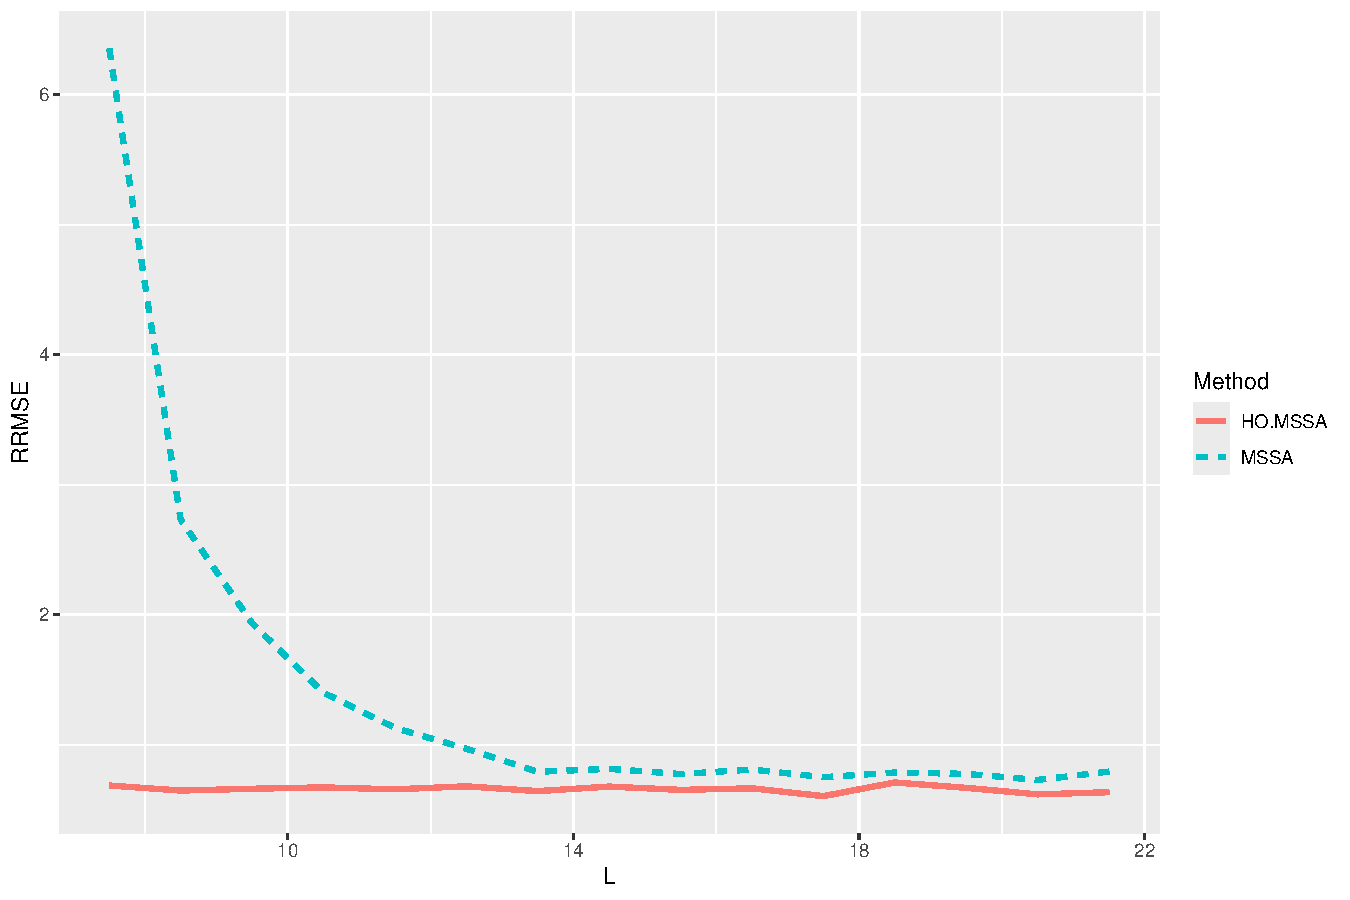
\includegraphics[width=\linewidth,
    height=0.167\textheight]{freq1_L_large_eq_rates.pdf}
    \caption{RRMSE оценок $\omega_1$.}
    \label{fig:freq1_L_large_eq_rates}
  \end{subfigure}
  \begin{subfigure}{0.49\linewidth}
    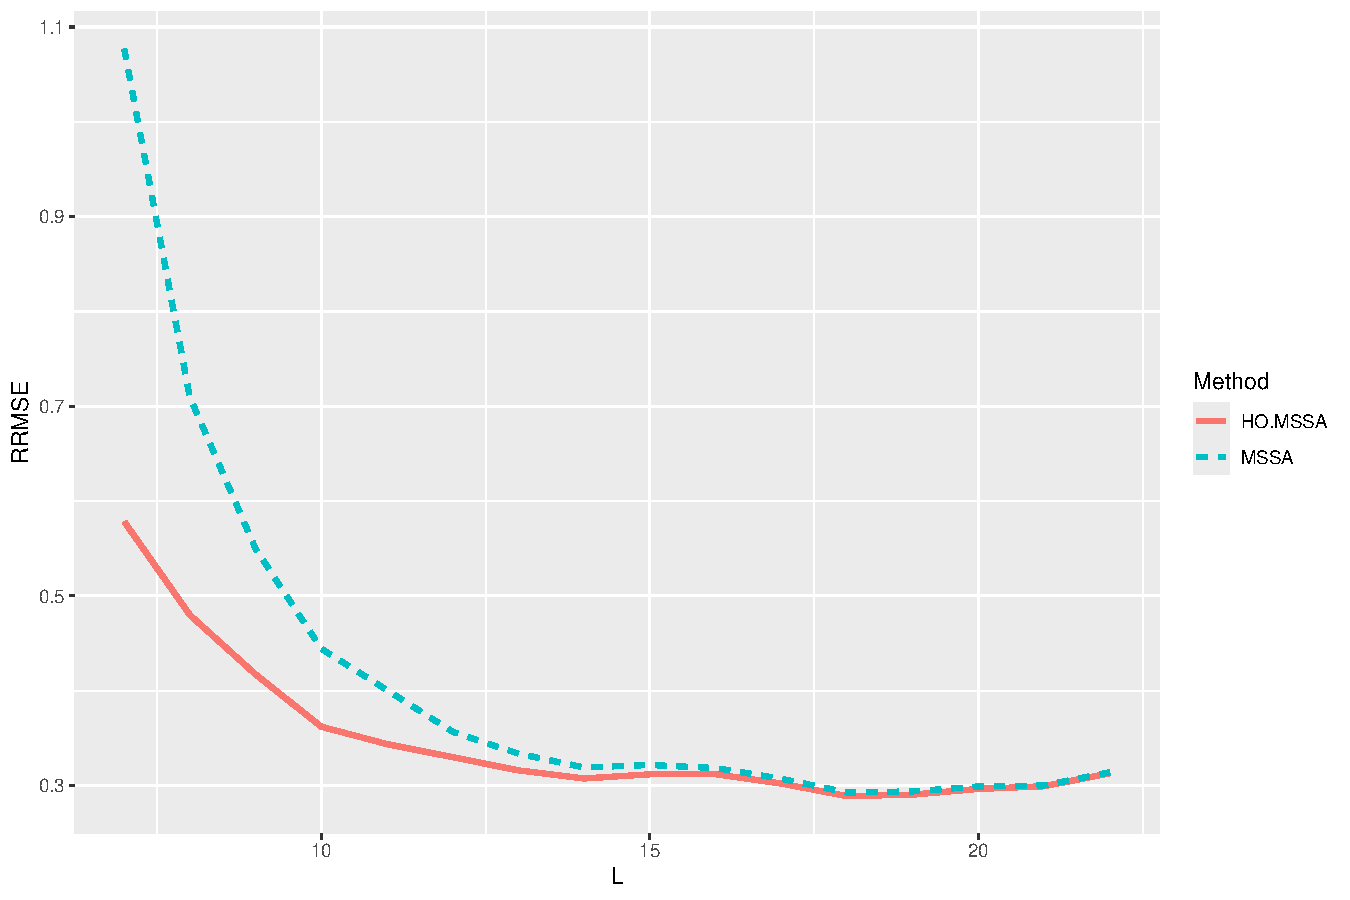
\includegraphics[width=\linewidth,
    height=0.167\textheight]{freq2_L_large_eq_rates.pdf}
    \caption{RRMSE оценок $\omega_2$.}
    \label{fig:freq2_L_large_eq_rates}
  \end{subfigure}
  \caption{Зависимость RRMSE оценок параметров многомерного ряда от
    длины окна,
  случай~\ref{enum:esprit-bigeq-rates}.}
  \label{fig:L_large_eq_rates}
\end{figure}

\begin{figure}[!ht]
  \centering
  \begin{subfigure}{0.49\linewidth}
    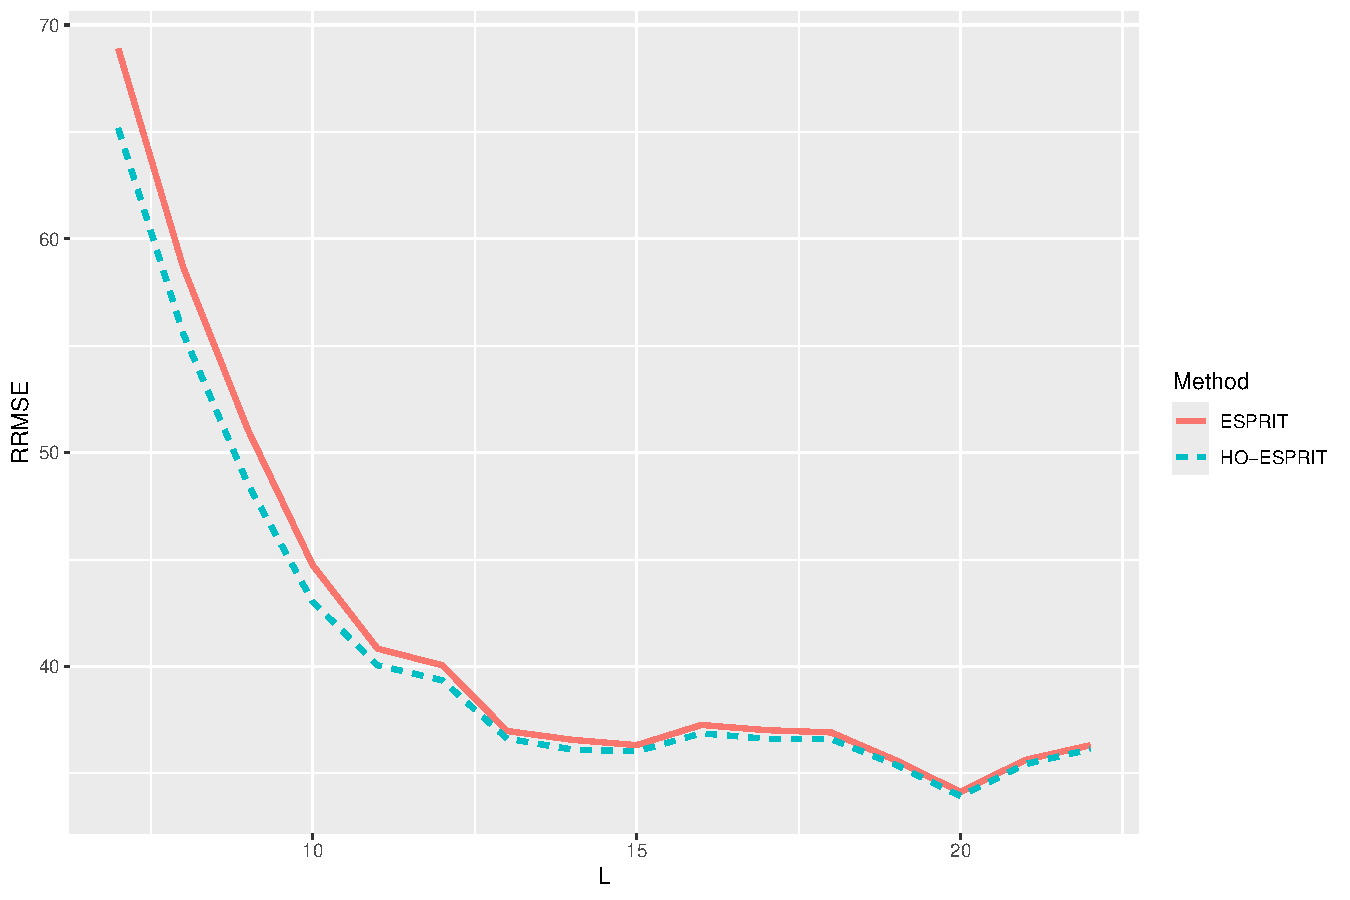
\includegraphics[width=\linewidth, height=0.167\textheight]{rate1_L.pdf}
    \caption{RRMSE оценок $\alpha_1$.}
    \label{fig:rate1_L}
  \end{subfigure}
  \begin{subfigure}{0.49\linewidth}
    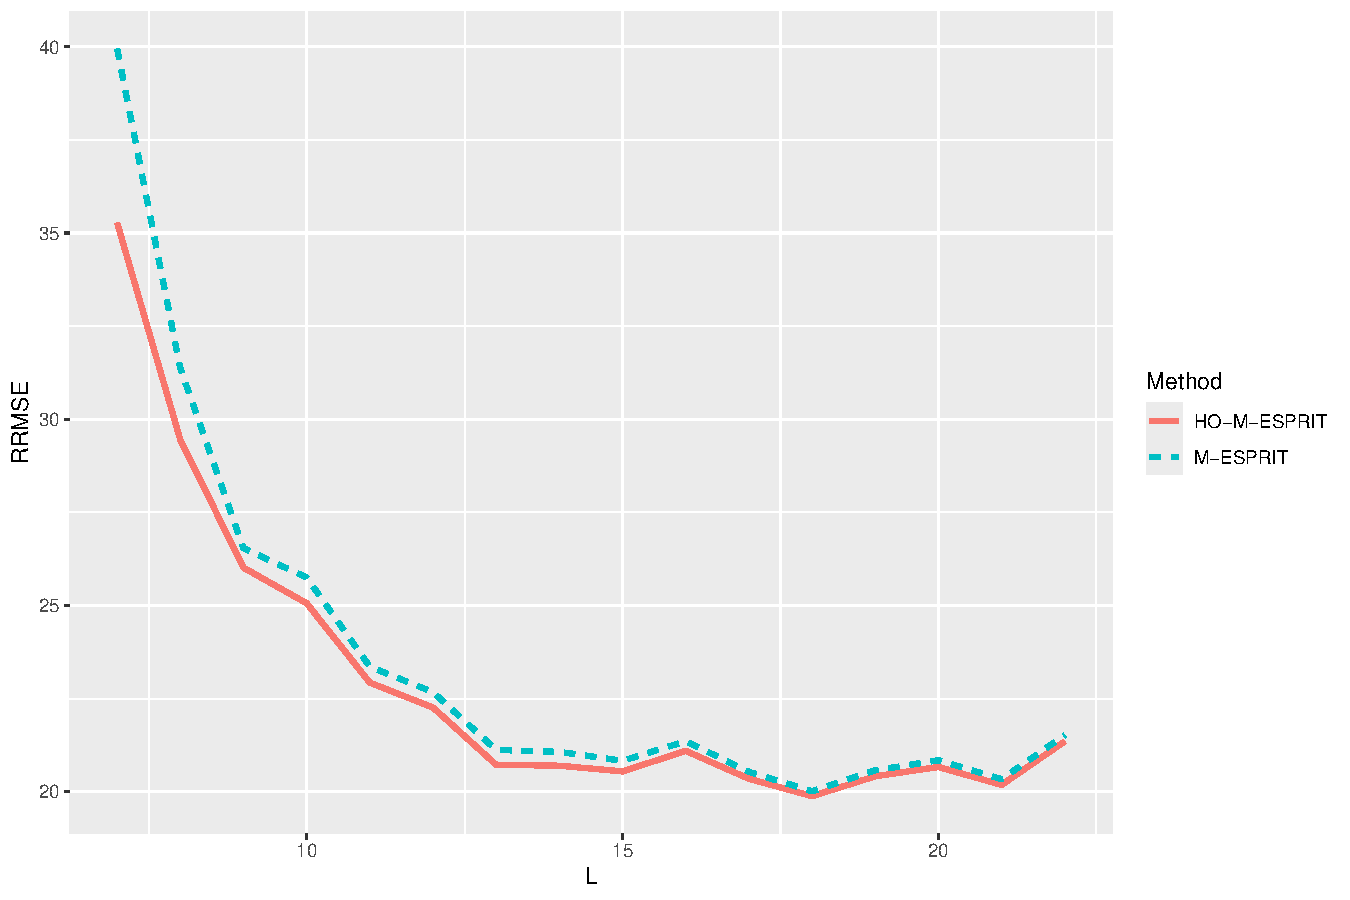
\includegraphics[width=\linewidth, height=0.167\textheight]{rate2_L.pdf}
    \caption{RRMSE оценок $\alpha_2$.}
    \label{fig:rate2_L}
  \end{subfigure}
  \begin{subfigure}{0.49\linewidth}
    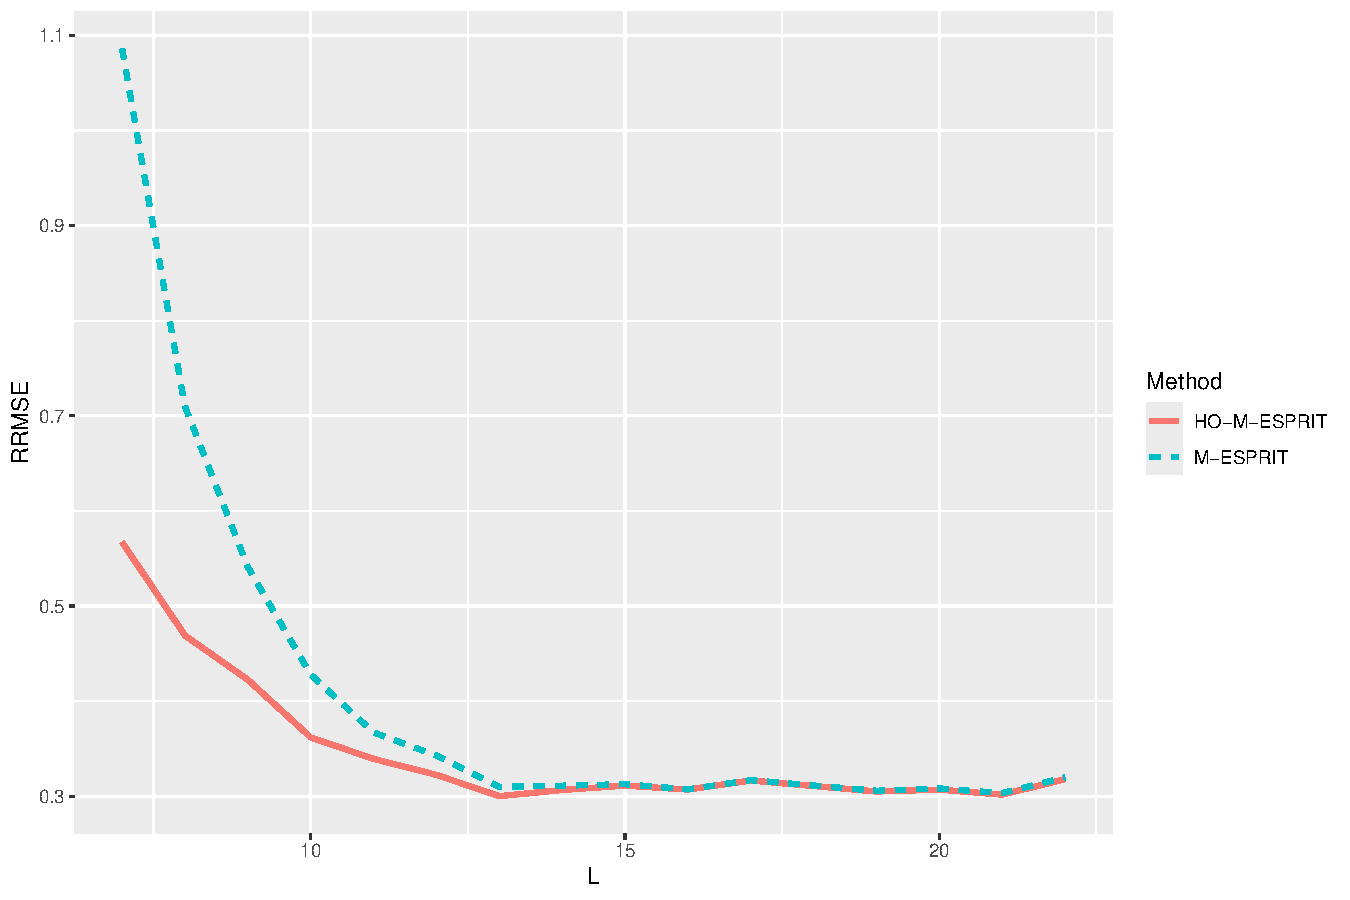
\includegraphics[width=\linewidth, height=0.167\textheight]{freq1_L.pdf}
    \caption{RRMSE оценок $\omega_1$.}
    \label{fig:freq1_L}
  \end{subfigure}
  \begin{subfigure}{0.49\linewidth}
    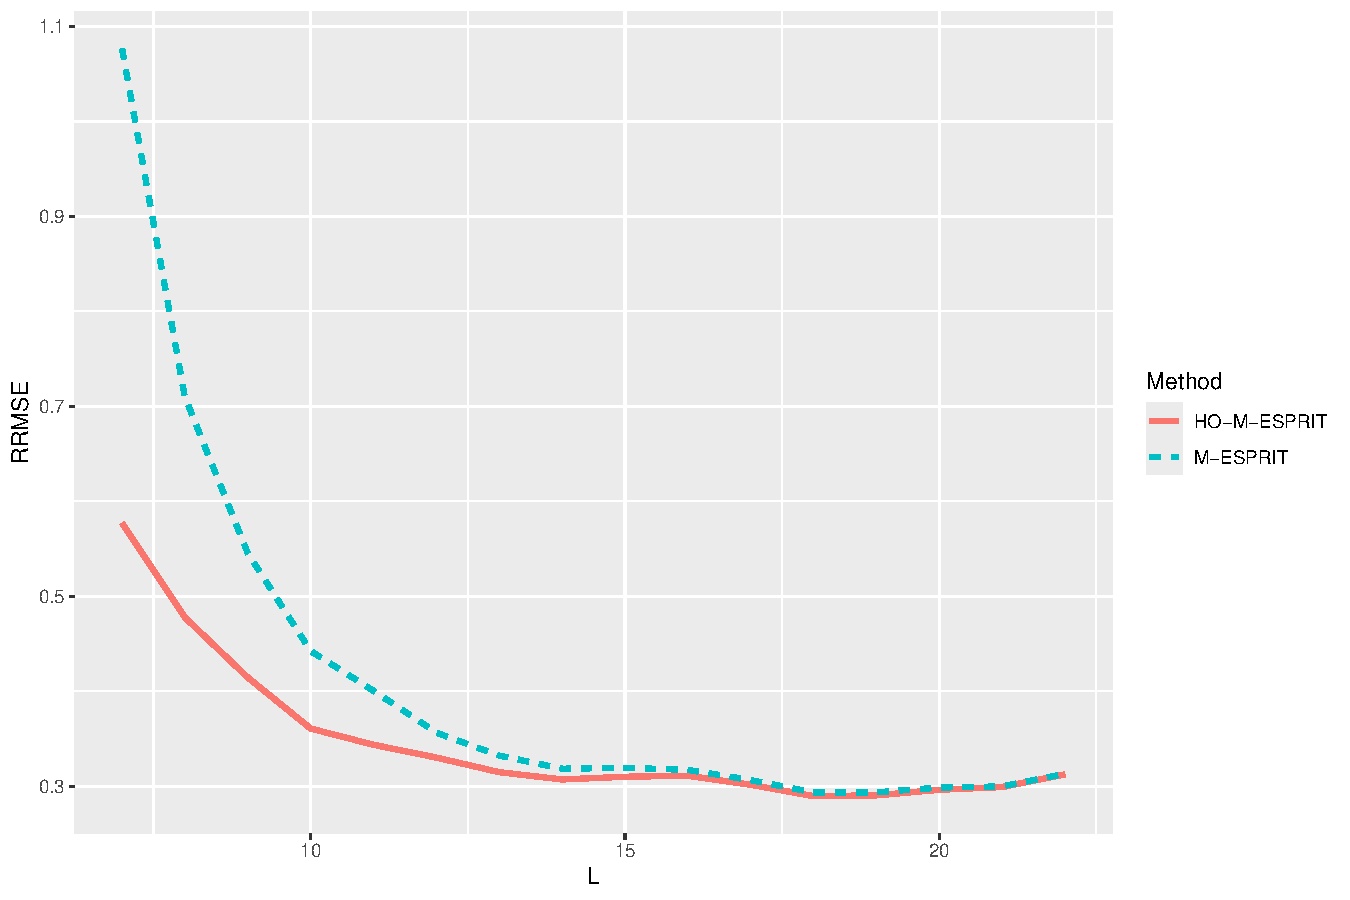
\includegraphics[width=\linewidth, height=0.167\textheight]{freq2_L.pdf}
    \caption{RRMSE оценок $\omega_2$.}
    \label{fig:freq2_L}
  \end{subfigure}
  \caption{Зависимость RRMSE оценок параметров многомерного ряда от
    длины окна,
  случай~\ref{enum:esprit-diff-rates}.}
  \label{fig:L_diff_rates}
\end{figure}

\paragraph{Выводы из численных сравнений}
Метод HO-M-ESPRIT оказался точнее стандартного метода M-ESPRIT в задаче
оценки параметров
многомерного ряда для любого выбора параметров длины окна во всех случаях,
не считая двух: оценки методом HO-M-ESPRIT параметра $\alpha_1$ оказались
менее точными, чем методом M-ESPRIT, в случаях~\ref{enum:esprit-smalleq-rates}
и~\ref{enum:esprit-bigeq-rates}.
Стоит заметить, что значения точности методов во всех случаях практически
не отличимы при больших значениях длины окна.

\section{Выбор направления усечения в алгоритме
HO-SSA}\label{sec:trunc-dim-ho-ssa}
В этом разделе рассматривается влияние выбора направлений усечения
в методе HO-SSA на точность в задаче выделения сигнала.

Пусть временной ряд $\tX$ имеет вид
\begin{gather*}
  \tX = (x_1, x_2,\ldots x_{N}), \\
  x_n = s_n + \varepsilon_n, \qquad n\in \overline{1:N},
\end{gather*}
где $\tS = (s_1, s_2, \ldots, s_N)$ "--- сигнал,
$\tE = (\varepsilon_1, \varepsilon_2, \ldots, \varepsilon_N)$ "--- шум.
Точность выделения сигнала будет оцениваться с помощью
среднеквадратичного отклонения (RMSE)
оценённого сигнала от исходного.
В данной работе RMSE высчитывается по следующей формуле
\begin{equation*}
  \text{RMSE} = \sqrt{\frac{1}{m} \sum_{i=1}^{m} \text{MSE}\left(\tS,
  \widetilde{\tS_i}\right)},
  \quad \text{MSE}\left(\tS, \widetilde{\tS} \right) = \frac{1}{N}
  \sum_{j=1}^{N}\left|s_j - \tilde{s}_j\right|^2,
\end{equation*}
где $m$ "--- количество реализаций шума, $\widetilde{\tS}_i$ "---
оценка сигнала,
восстановленная по ряду с $i$-й реализацией шума.
В качестве способа разложения траекторного тензора был выбран метод HOOI.

\subsection{Выделение вещественного сигнала}\label{subsec:comparison}
Пусть $N = 71$ и временной ряд состоит из элементов вида
\begin{equation}
  \label{eq:ho-ssa-sin-signal}
  x_n = 30\cos(2\pi n/12) + \varepsilon_n,
\end{equation}
где $\varepsilon_n$ "--- независимые случайные величины из
распределения $\mathrm{N}(0, \sigma^2)$,
$\sigma^2=25$.
Во всех алгоритмах для восстановления бралось количество компонент
разложения равное рангу сигнала,
который в данном случае равен 2.
В таблице~\ref{tab:ssa-cos} приведены значения RMSE оценки сигнала,
восстановленного
методом SSA при различных выборах длины окна.
\begin{table}[!ht]
  \centering
  \caption{SSA: RMSE оценки сигнала~\eqref{eq:ho-ssa-sin-signal}.}
  \begin{tabular}{|r|r|r|r|r|}
    \hline
    $L$ &   12 &   24 &            30 &   36 \\ \hline
    RMSE & 1.82 & 1.42 & \textbf{1.40} & 1.42 \\ \hline
  \end{tabular}\label{tab:ssa-cos}
\end{table}
RMSE здесь и далее в этом разделе высчитывается по $m=500$ реализациям шума.
Кроме того, здесь и далее жирным шрифтом выделены минимальные по
строке значения RMSE, причём
отличие этих минимальных значений от остальных в строке значимо при
уровне значимости $\alpha = 0.05$.

В таблице~\ref{tab:sin-rec-dims} представлены значения RMSE оценок
сигнала, восстановленного методом HO-SSA при
выборе различных направлений усечения.
Параметры в таблице~\ref{tab:sin-rec-dims} представлены в порядке
уменьшения третьего размера
траекторного тензора, причём выполняется неравенство $I \leqslant J
\leqslant L$.
Б\'{о}льшие параметры длин окна не рассматриваются, так как построенные по ним
траекторные матрицы и траекторные тензоры будут совпадать с
рассмотренными с точностью
до перестановки размерностей.
\begin{table}[!ht]
  \centering
  \caption{HO-SSA: RMSE оценки сигнала~\eqref{eq:ho-ssa-sin-signal} при
  выборе разных направлений усечения.}\label{tab:sin-rec-dims}
  \begin{tabular}{|c|c|c|c|c|c|c|}
    \hline
    \backslashbox{
      \renewcommand{\arraystretch}{0.72}
      \begin{tabular}{ll}Направления\\усечения
    \end{tabular}}{$I\times L$}& $12{\times}49$ & $12{\times}37$ &
    $7{\times}36$
    & $12{\times}31$ & $19{\times}30$ & $24{\times}25$ \\
    \hline
    3 & 1.85 & 1.52 & \textbf{1.48} & 1.54 & 1.57 & 1.59\\ \hline
    2, 3 & 1.63 & 1.53 & \textbf{1.49} & 1.56 & 1.62 & 1.65 \\ \hline
    $\overline{1:3}$ & 1.63 & 1.53 & \textbf{1.49} & 1.56 & 1.62 & 1.65 \\
    \hline
  \end{tabular}
\end{table}

Из таблицы~\ref{tab:sin-rec-dims} видно, что усечение только по
направлению наибольшей размерности
даёт результаты точнее, чем усечение по всем направлениям, при почти
любом выборе
длин окна.
Но этого увеличения точности недостаточно, чтобы алгоритм HO-SSA был
точнее базового SSA.

\subsection{Выделение комплексного
сигнала}\label{subsec:complex-signal-extraction}
Рассмотрим задачу выделения комплекснозначного сигнала из ряда $\tX$
с элементами вида~\eqref{eq:esprit-1d-series}
с частотами $\omega_1 = 0.2$, $\omega_2 = 0.22$ и со степенями
затухания $\alpha_1=-0.01$,
$\alpha_2 = -0.02$.

На рисунке~\ref{fig:rec-dims} представлен график зависимости RMSE от размеров
траекторного тензора (ось $x$) и направлений усечения (цвет и тип линий).
Чёрной пунктирной линией на графике изображено минимальное по
выбору длины окна
значение RMSE для сигналов, восстановленных методом SSA.
\begin{figure}[!ht]
  \centering
  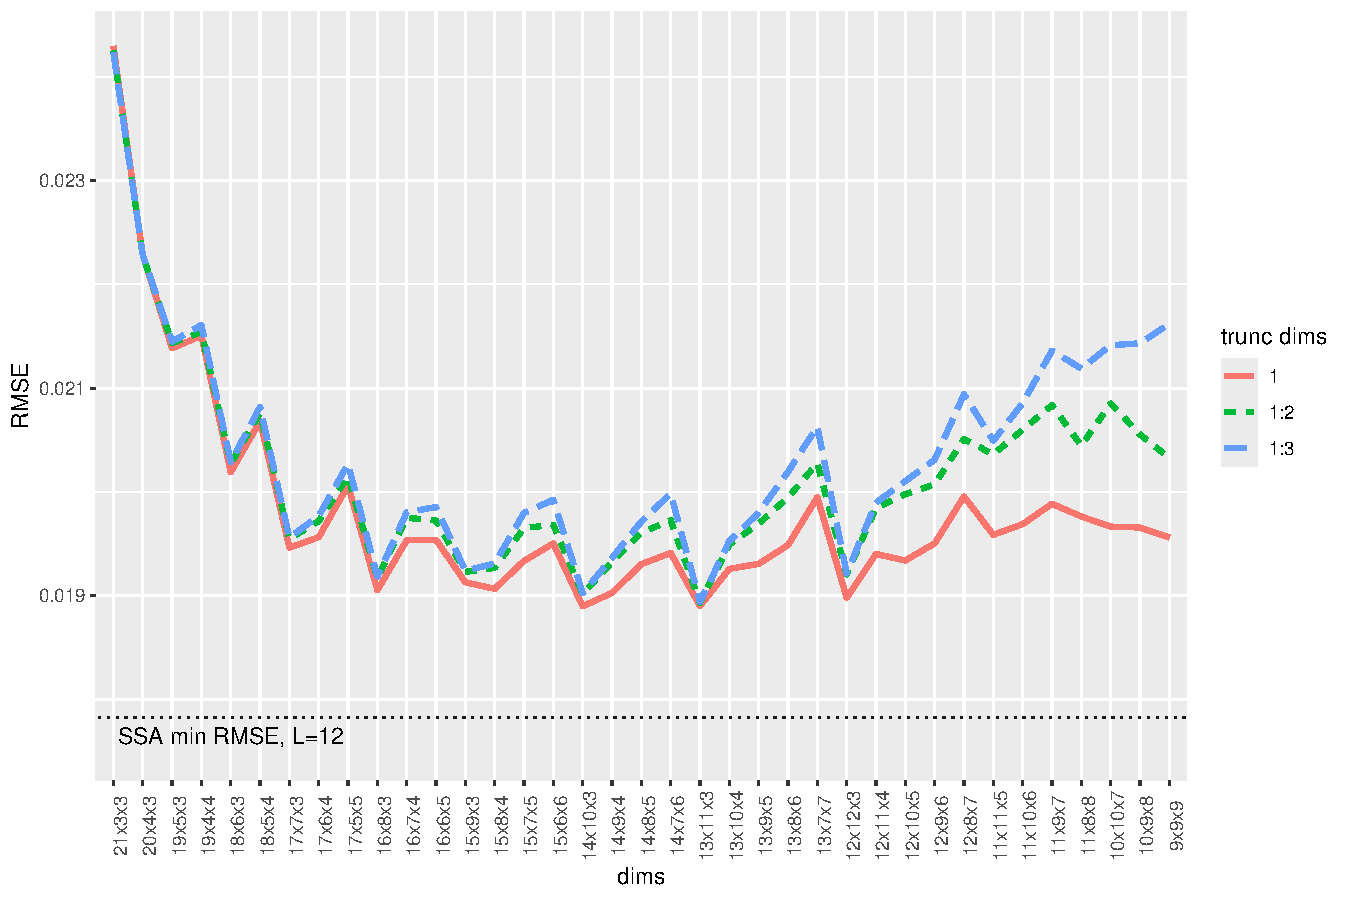
\includegraphics[width=\textwidth, height=0.38\textheight]{rec_dim_rmse}
  \caption{Зависимость RMSE восстановленного сигнала от размеров
    траекторного тензора
  и направлений усечений.}\label{fig:rec-dims}
\end{figure}
Как и в случае вещественного сигнала, метод HO-SSA оказывается
существенно менее точным при
любом выборе длин окна и направлений усечения, чем метод SSA.
Также наиболее точные оценки сигнала получаются при выборе в качестве
направления усечения направления минимальной размерности траекторного
тензора ряда.

\paragraph{Выводы численных сравнений}
В отличие от задачи оценки параметров, где при выборе оптимальных длин окна
тензорные методы могут давать оценки точнее, чем базовый ESPRIT, в
задаче выделения
сигнала при любом выборе длин окна точность восстановленных тензорными
методами оценок сигналов всегда существенно меньше точности оценок,
восстановленных
базовым SSA.

\section{Численные сравнения в задаче выделения многомерных
комплексных сигналов}\label{sec:cmssa-comparison}
Пусть многомерный временной ряд $\tX$ имеет тот же вид, что и ряд,
рассматриваемый в разделе~\ref{subsec:mv-esprit-comparison}.
Рассмотрим задачу выделения сигнала из этого временного ряда.

Ранг этого сигнала в терминах MSSA при всех рассматриваемых
вариантах параметров $\alpha_1$ и $\alpha_2$ равен 2, поэтому
параметр $R$ в алгоритме MSSA
и параметры $R_1$ и $R_2$ в алгоритме~\ref{alg:ho-mssa-signal} были
взяты равными 2.
3-ранг этого сигнала в терминах HO-MSSA равен 2, поэтому параметр
$R_3$ в алгоритме~\ref{alg:ho-mssa-signal} был взят равным 2.
Случаи усечения по части направлений не рассматривались в силу
замечания~\ref{remark:ho-mssa-trunc-dims}.

\begin{figure}
  \centering
  \begin{subfigure}{0.49\linewidth}
    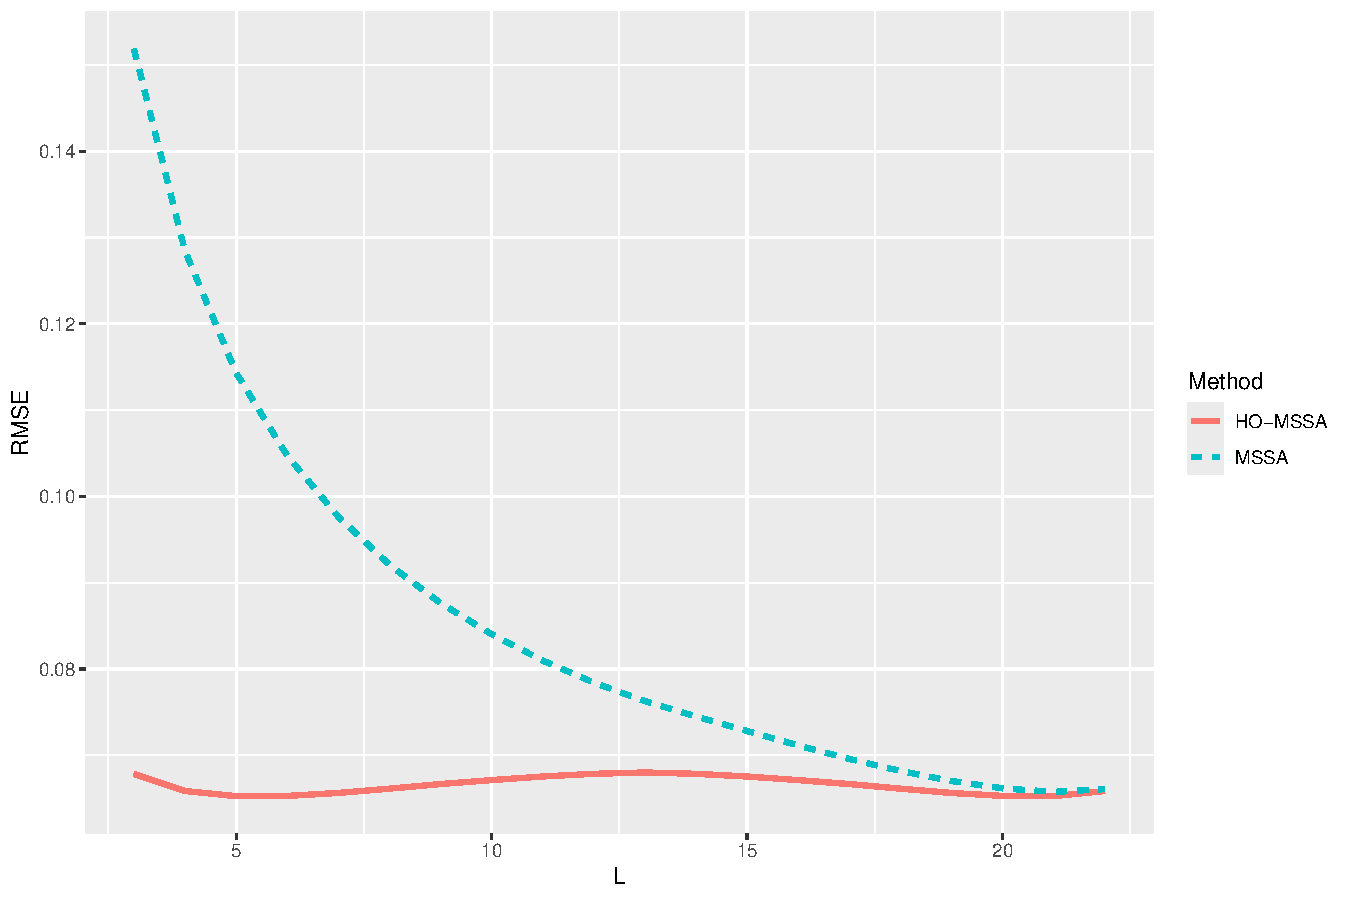
\includegraphics[width=\linewidth,
    height=0.167\textheight]{rec_L_rmse_no_rates.pdf}
    \caption{$\alpha_1$ и $\alpha_2$ из случая \ref{enum:esprit-no-rates}.}
    \label{fig:L_rmse_no_rates}
  \end{subfigure}
  \begin{subfigure}{0.49\linewidth}
    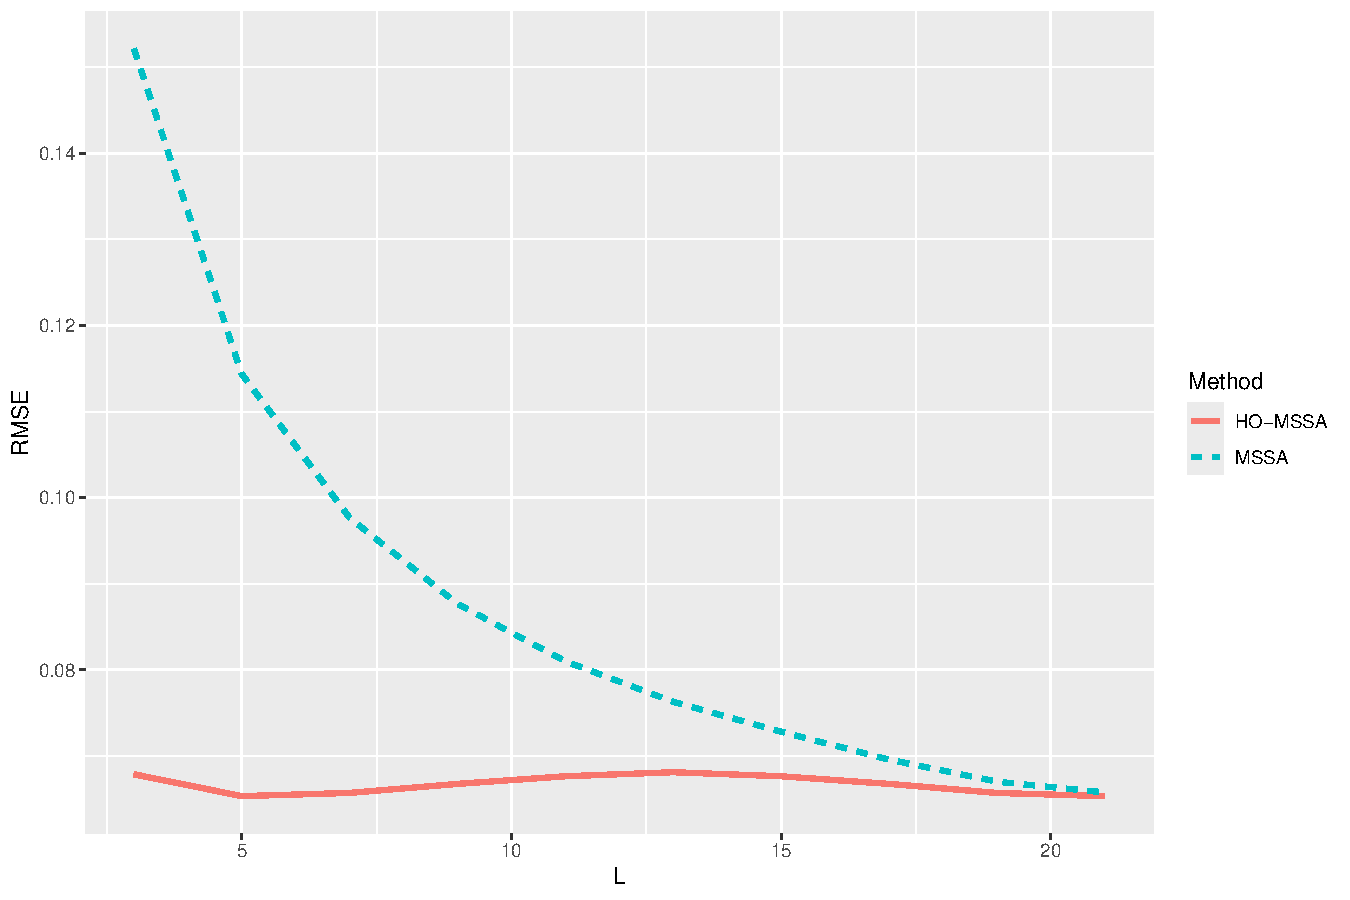
\includegraphics[width=\linewidth,
    height=0.167\textheight]{rec_L_rmse_small_eq_rates.pdf}
    \caption{$\alpha_1$ и $\alpha_2$ из случая
    \ref{enum:esprit-smalleq-rates}.}
    \label{fig:L_rmse_smalleq_rates}
  \end{subfigure}
  \begin{subfigure}{0.49\linewidth}
    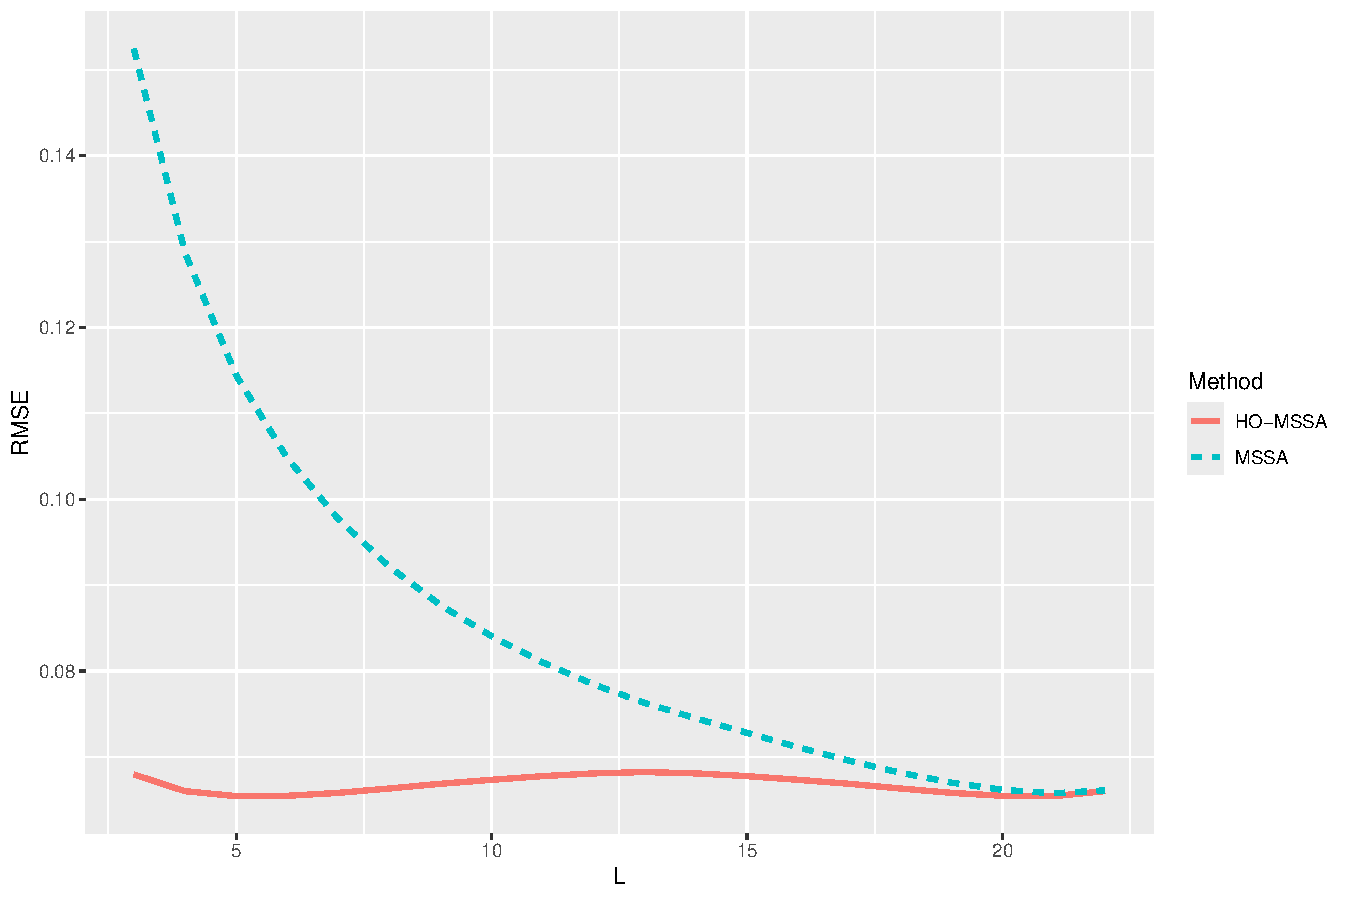
\includegraphics[width=\linewidth,
    height=0.167\textheight]{rec_L_rmse_large_eq_rates.pdf}
    \caption{$\alpha_1$ и $\alpha_2$ из случая \ref{enum:esprit-bigeq-rates}.}
    \label{fig:L_rmse_bigeq_rates}
  \end{subfigure}
  \begin{subfigure}{0.49\linewidth}
    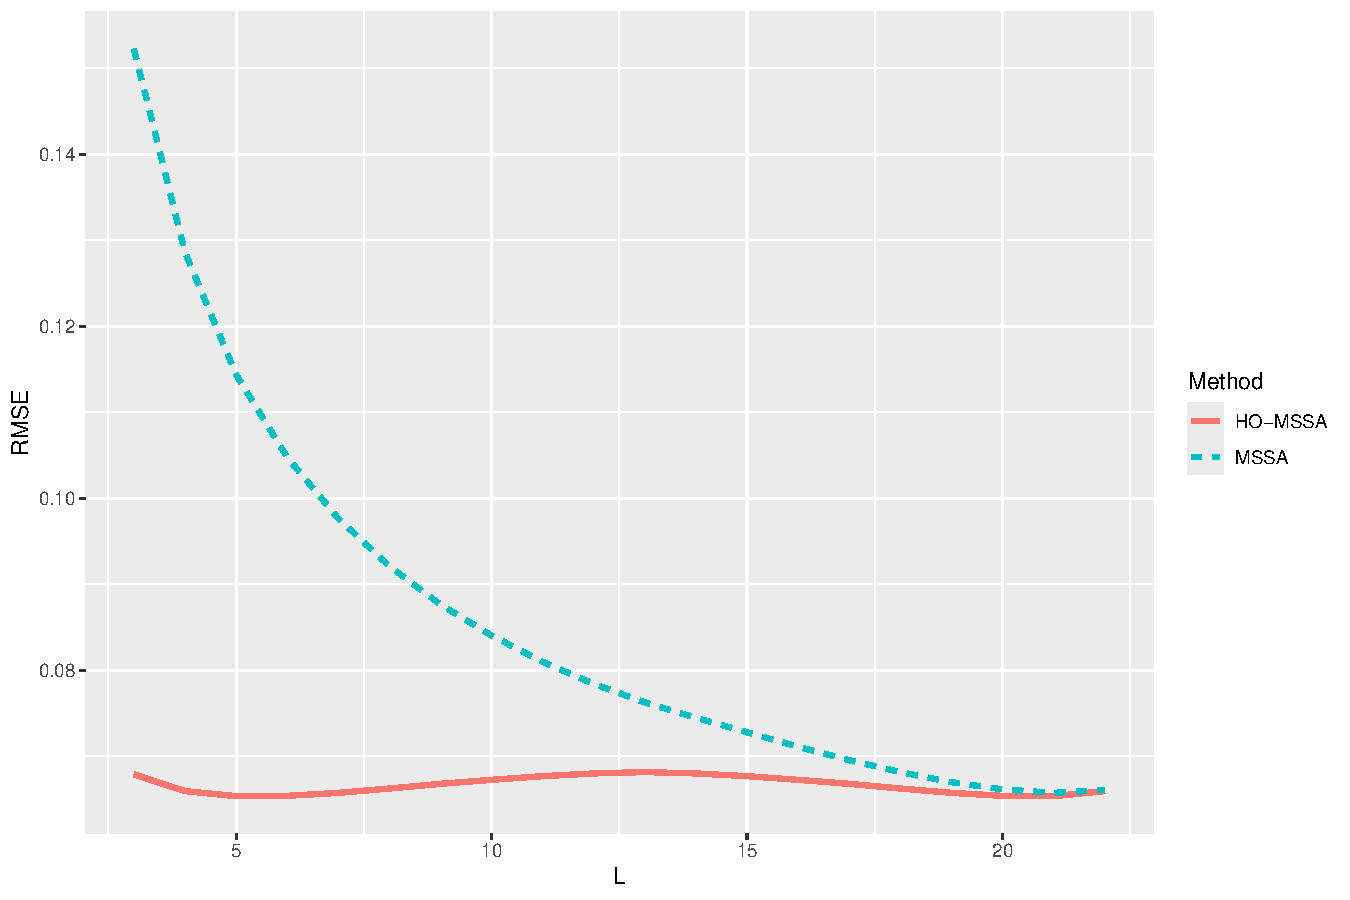
\includegraphics[width=\linewidth,
    height=0.167\textheight]{rec_L_rmse.pdf}
    \caption{$\alpha_1$ и $\alpha_2$ из случая \ref{enum:esprit-diff-rates}.}
    \label{fig:L_rmse_diff_rates}
  \end{subfigure}
  \caption{Зависимость RMSE оценок многомерного сигнала от длины окна.}
  \label{fig:mv_L_rmse}
\end{figure}
На рисунках~\ref{fig:mv_L_rmse} приведены графики
зависимости RMSE оценок
сигнала методами MSSA и HO-MSSA от выбора длины окна $L$ для различных
параметров степеней затухания $\alpha_1$ и $\alpha_2$.

Из графиков видно, что во всех случаях метод HO-MSSA выделяет
комплексный сигнал более точно, чем метод MSSA,
причём преимущество велико для большинства значений длины окна $L$.
Однако RMSE обоих методов при оптимальном выборе $L$ довольно близки.
Этот результат совпадает с результатами численного сравнения методов MSSA и
HO-MSSA в задаче выделения вещественных сигналов.

Метод MSSA имеет асимптотическую трудоёмкость $O(LKPr)$, где
$r$ "--- количество компонент SVD, по которым оценивается сигнал.
Из рисунков видно, что наибольшей точности метод достигает при
$L \approx N-r$.
Тогда, учитывая, что $K=N - L + 1$ и $r\ll N$, трудоёмкость MSSA
можно переписать в виде $O(NPr^2)$.
Метод HO-MSSA с использованием HOOI имеет асимптотическую
трудоёмкость $O(LKP(2r+r_3))$, где $r$ "--- количество
компонент первых двух направлений HOSVD,
по которым оценивается сигнал, а $r_3$ "--- количество компонент
третьего направления.
Метод HO-MSSA обладает свойством симметричности относительно
замены $L$ на $K=N-L+1$ в том смысле, что применение алгоритма
с параметром длины окна $L$ или $K$ даёт одинаковые оценки,
поэтому графики RMSE, соответствующие методу HO-MSSA
на рисунке~\ref{fig:mv_L_rmse} симметричны относительно $N/2$.
Трудоёмкость алгоритма HO-MSSA также симметрична относительно
замены $L$ на $K$.
Наибольшей точности алгоритм достигает также при
$L\approx N - r$, поэтому трудоёмкость HO-MSSA в этом случае можно переписать
как $O(NPr(2r+r_3))$.
Таким образом, хоть метод HO-MSSA более точен, он также более
трудоёмкий, чем MSSA.

\section{Численные сравнения методов Dstack со
стандартными}\label{sec:dstack-comparison}
Рассмотрим случай временного ряда, состоящего из двух гармоник с
близкими частотами.
Особенность близких частот в том, что с увеличением шума некоторые
методы оценки параметров могут начать идентифицировать обе частотные
компоненты как одну с параметрами, равными усреднённым значениям
параметров исходных компонент.
Пусть ряд $\tX$ состоит
из элементов вида
\[
  x_{n + 1} = \cos\left(2 \pi n \omega_1\right) + \cos\left(2 \pi n
  \omega_2\right) + \xi_n,
\]
где $\omega_1 = 0.02$, $\omega_2 = 0.0205$, $\xi_n$ "--- независимые
случайные величины из распределения $\rmN(0, \sigma^2)$, $n \in
\overline{0:989}$.
Ранг этого ряда в терминах SSA равен 4, поэтому в задаче оценки
параметров выбирается $R=4$ в
алгоритмах~\ref{alg:ssa-signal},~\ref{alg:esprit},~\ref{alg:dstack-ho-esprit},
и $R_1=R_2 = 4$ в алгоритме~\ref{alg:dstack-ho-ssa}.
Во всех случаях для Dstack методов был выбран параметр $D=10$.
В этом случае $\max_j |\omega_j| = 0.0205 \leqslant 0.05 = 1 / 2D$,
то есть выполняются условия из замечания~\ref{remark:dstack_condition},
значит Dstack методы применимы.
Ряд был выбран аналогично тому, что рассматривался в работе~\cite{Papy2009}.

В этом разделе точность выделения частот и оценки сигнала
оценивается с помощью RMSE, посчитанного по 100 реализациям шума.
RMSE оценки частоты сигнала считается следующим образом
\begin{equation}
  \label{eq:rmse-estim}
  \operatorname{RMSE} =\sqrt{\frac{1}{2m}
    \sum_{k=1}^{2}\sum_{j=1}^{m}
  \left|\omega_{k}-\widehat{\omega}_{kj}\right|^2},
\end{equation}
где $\widehat{\omega}_{kj}$ "--- оценка частоты $\omega_k$, полученная по ряду
с $j$-й реализацией шума.
Так как ранг рассматриваемого временного ряда равен 4, то методы,
основанные на подпространстве сигнала, возвращают 4 оценки параметров.
В случае отсутствия шума множество оценок можно разбить на две группы с равными
параметрами $\alpha$ и равными по модулю параметрами $\omega$.
В связи с этим на множестве модулей полученных оценок частот
проводилась кластеризация методом kmeans, в качестве
$\widehat{\omega}_{1j}$ выбирался наименьший по значению центр
кластера, а в качестве
$\widehat{\omega}_{2j}$ --- наибольший.

\subsection{Задача оценки параметров сигнала}\label{subsec:dstack-esprit}
Сравниваются методы ESPRIT, Dstack ESPRIT и два варианта Dstack
HO-ESPRIT: с выбором $R_3=4$ и $R_3=1$.
Выбор $R_3=4$ обусловлен тем, что 3-ранг ряда
$\tX_D=\calD_D(\tX)$ равен 4, а выбор $R_3=1$ обусловлен
теоремой~\ref{theorem:ho-m-esprit-r3}.

Рассматриваются два варианта шума: <<малый>> --- со стандартным
отклонением \linebreak$\sigma=0.2$,
и <<большой>> --- с $\sigma = 0.6$.
На рисунках~\ref{fig:dstack-esprit-byL-small} приведены графики
зависимости RMSE оценки методом ESPRIT (слева) и Dstack модификациями
(справа) от длины окна для малого шума, а на
рисунках~\ref{fig:dstack-esprit-byL-large} "--- для большого.
Для удобства сравнения на каждом из графиков
пунктирной линией обозначено минимальное значение с соседнего графика.
\begin{figure}[!ht]
  \begin{minipage}{0.48\textwidth}
    \centering
    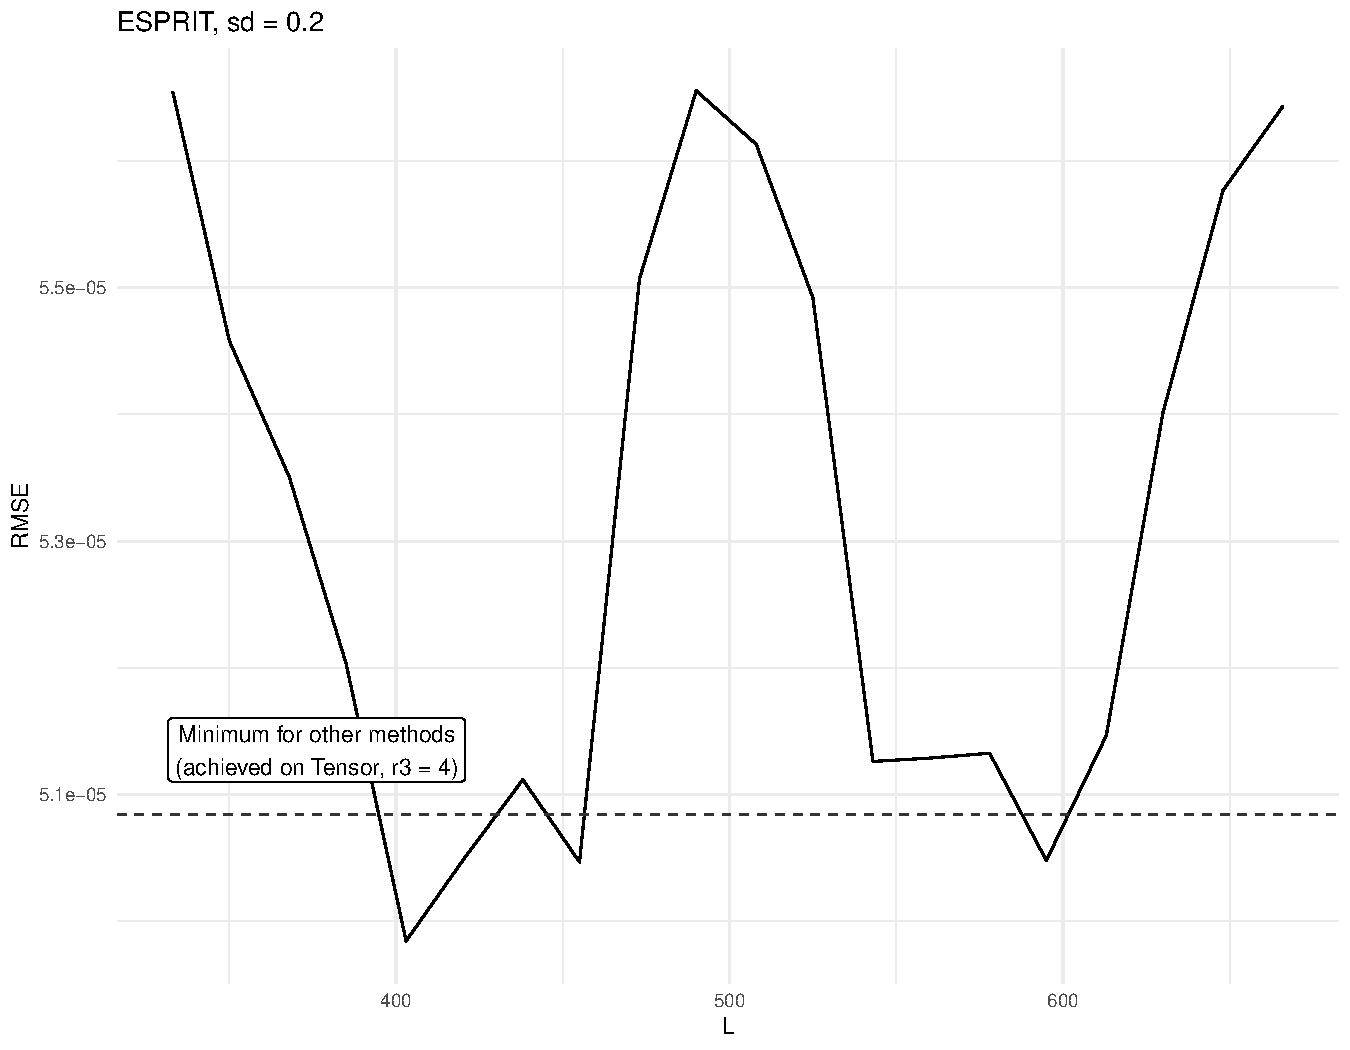
\includegraphics[width=\textwidth]{htlsd_byL_real_param_rmse_esprit_2.pdf}
  \end{minipage}
  \begin{minipage}{0.48\textwidth}
    \centering
    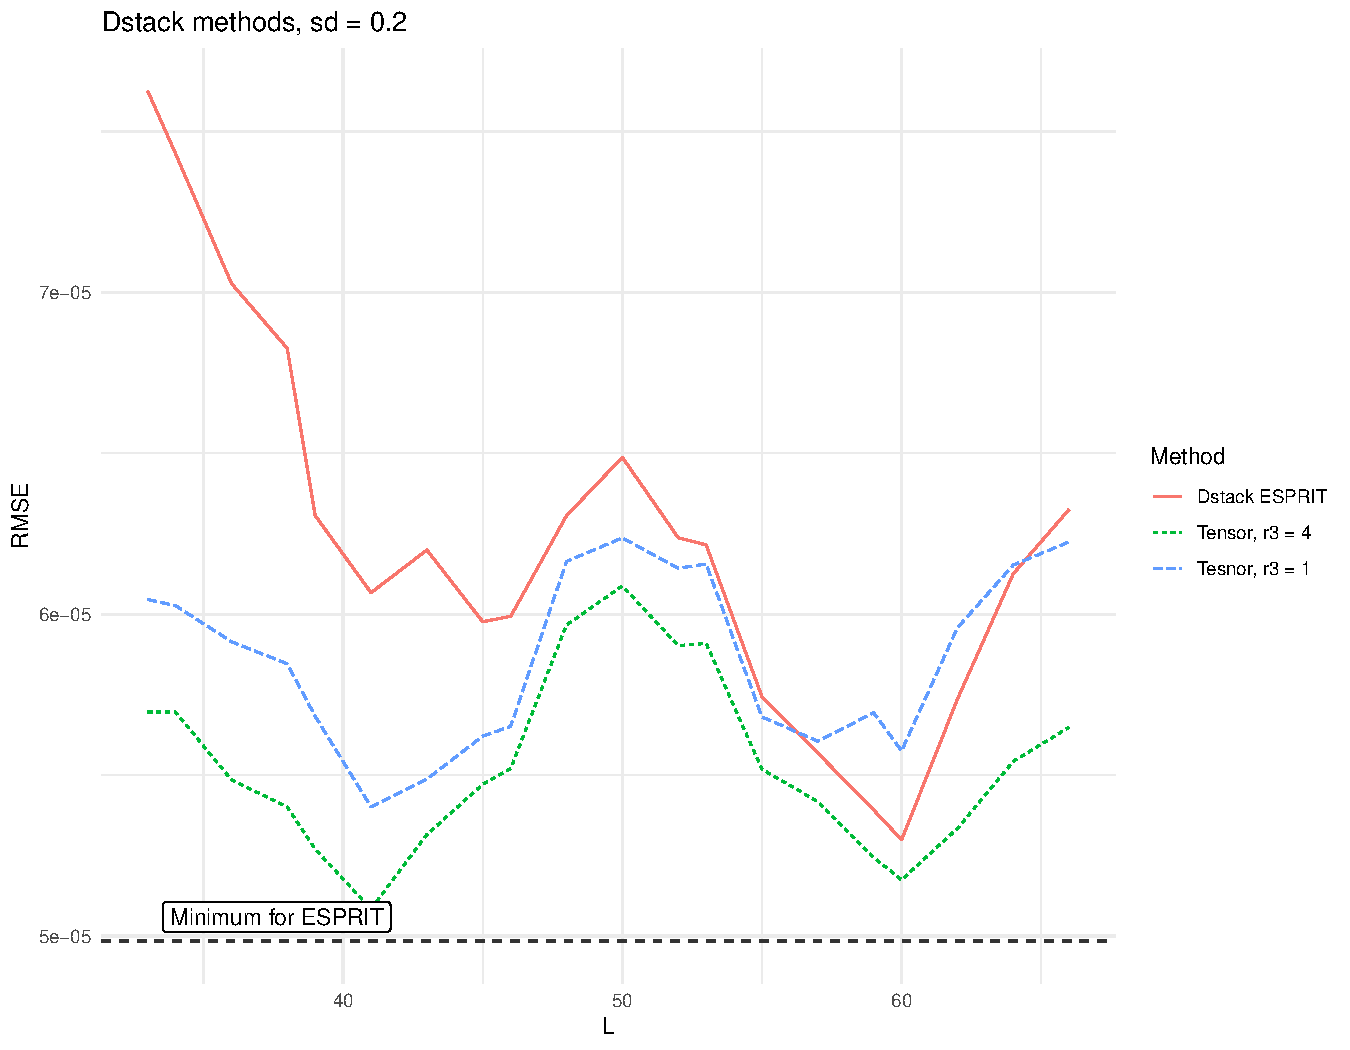
\includegraphics[width=\textwidth]{htlsd_byL_real_param_rmse_dstack_2.pdf}
  \end{minipage}
  \caption{Зависимость RMSE оценки частот методами ESPRIT и
  модификациями Dstack от длины окна. Случай $\sigma = 0.2$.}
  \label{fig:dstack-esprit-byL-small}
\end{figure}
\begin{figure}
  \begin{minipage}{0.48\textwidth}
    \centering
    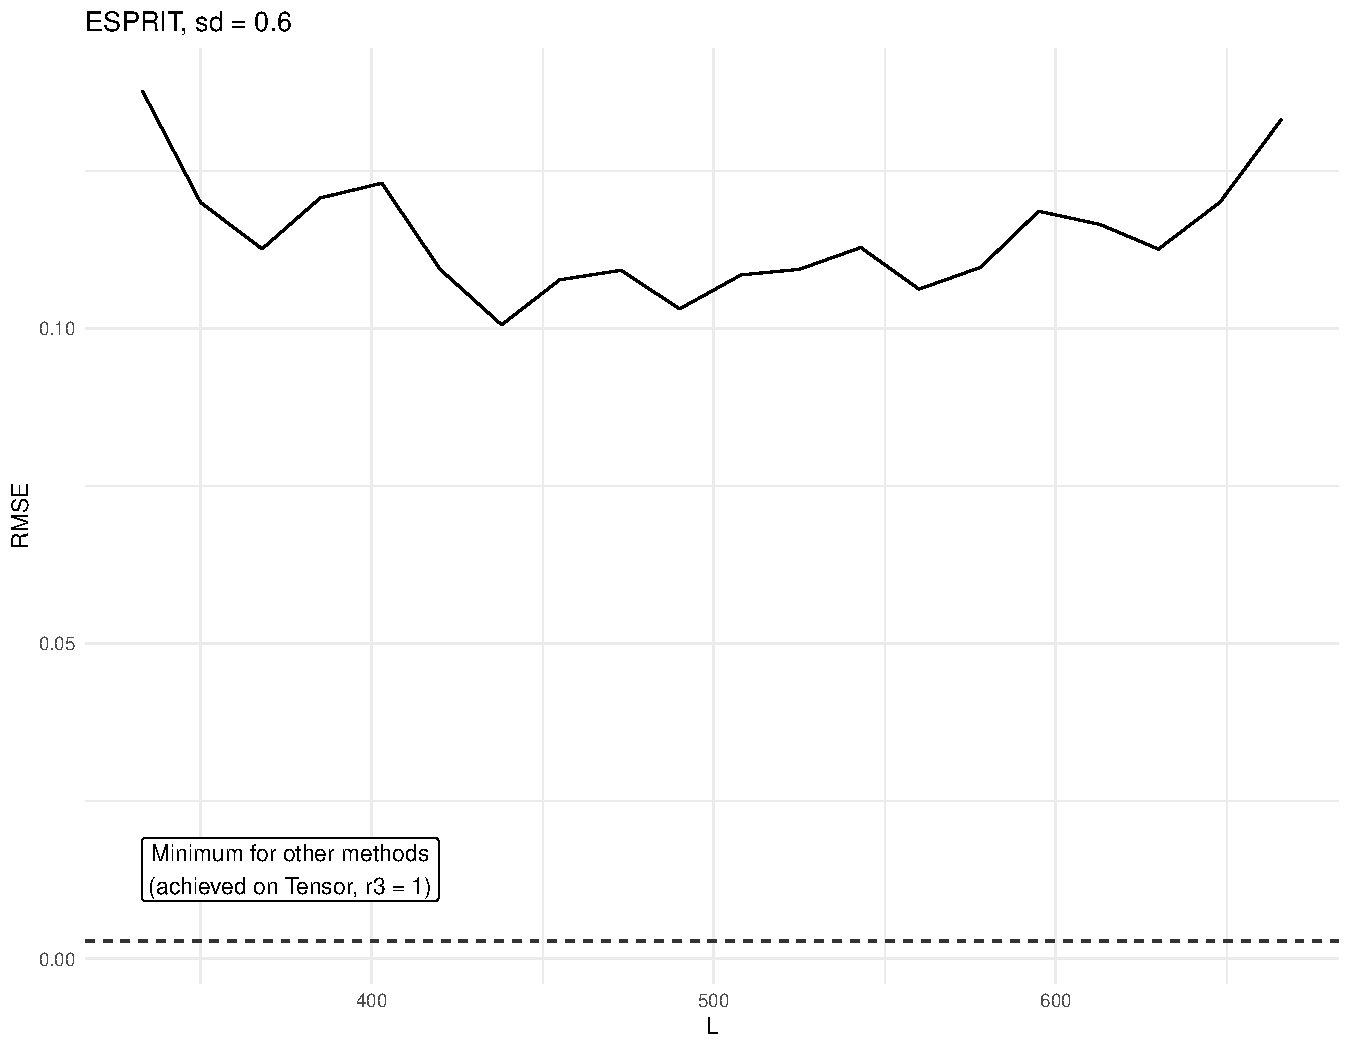
\includegraphics[width=\textwidth]{htlsd_byL_real_param_rmse_esprit_3.pdf}
  \end{minipage}
  \begin{minipage}{0.48\textwidth}
    \centering
    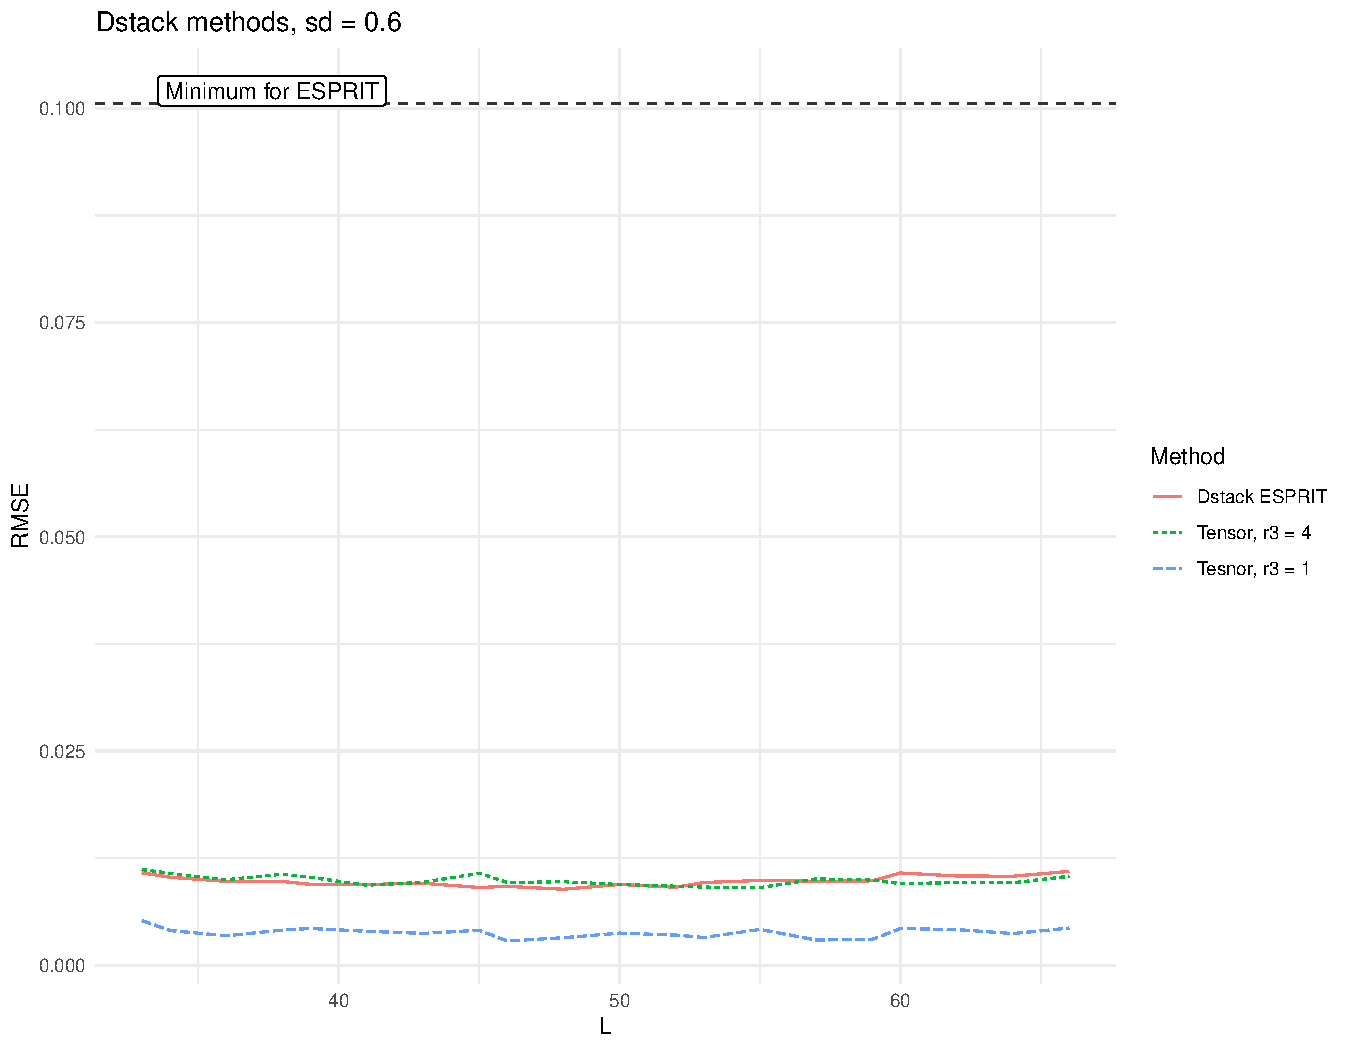
\includegraphics[width=\textwidth]{htlsd_byL_real_param_rmse_dstack_3.pdf}
  \end{minipage}
  \caption{Зависимость RMSE оценки частот методами ESPRIT и
  модификациями Dstack от длины окна. Случай $\sigma = 0.6$.}
  \label{fig:dstack-esprit-byL-large}
\end{figure}

Из графиков видно, что при малом уровне шума все методы близки по
точности, и минимальная ошибка достигается методом ESPRIT, а среди
Dstack методов наименьшую ошибку имеет Dstack HO-ESPRIT с выбором $R_3=4$.
Однако в случае высокого уровня шума точность метода ESPRIT заметно снижается.
Это происходит по той причине, что из-за близости частот $\omega_1$ и
$\omega_2$ ESPRIT
перестаёт их различать, и оценивает как одну частоту.
Наиболее точным методом в случае большого уровня шума является Dstack
HO-ESPRIT с выбором $R_3=1$.

\subsection{Задача выделения сигнала}\label{subsec:dstack-signal}
Сравниваются методы SSA, Dstack SSA и Dstack
HO-SSA с выбором $R_3=4$.
Вариант $R_3=1$ не рассматривается, так как в этом случае, в отличие от задачи
оценки параметров, у оценки сигнала возникает большое смещение.

Как и в разделе~\ref{subsec:dstack-esprit}, рассматриваются два
уровня шума: $\sigma=0.2$ и $\sigma = 0.6$.
На рисунках~\ref{fig:dstack-ssa-byL-small} приведены графики
зависимости RMSE оценки методом SSA (слева) и Dstack модификациями
(справа) от длины окна для малого шума, а на
рисунках~\ref{fig:dstack-ssa-byL-large} "--- для большого.
Для удобства сравнения на каждом из графиков
пунктирной линией обозначено минимальное значение с соседнего графика.
\begin{figure}[!ht]
  \begin{minipage}{0.48\textwidth}
    \centering
    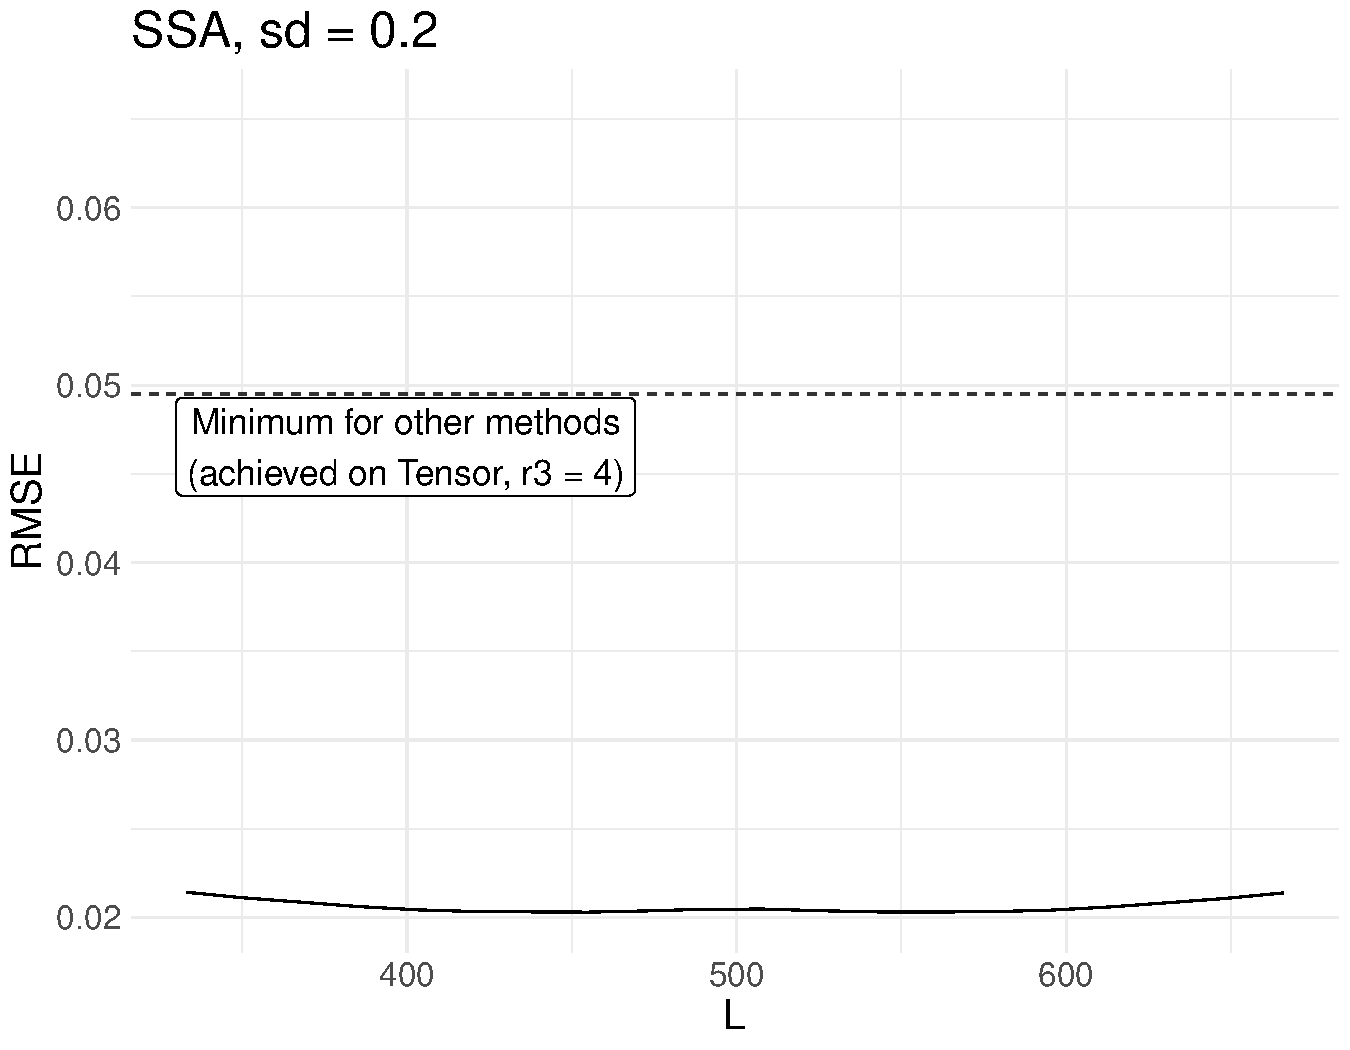
\includegraphics[width=\textwidth]{htlsd_byL_real_rec_rmse_ssa_2.pdf}
  \end{minipage}
  \begin{minipage}{0.48\textwidth}
    \centering
    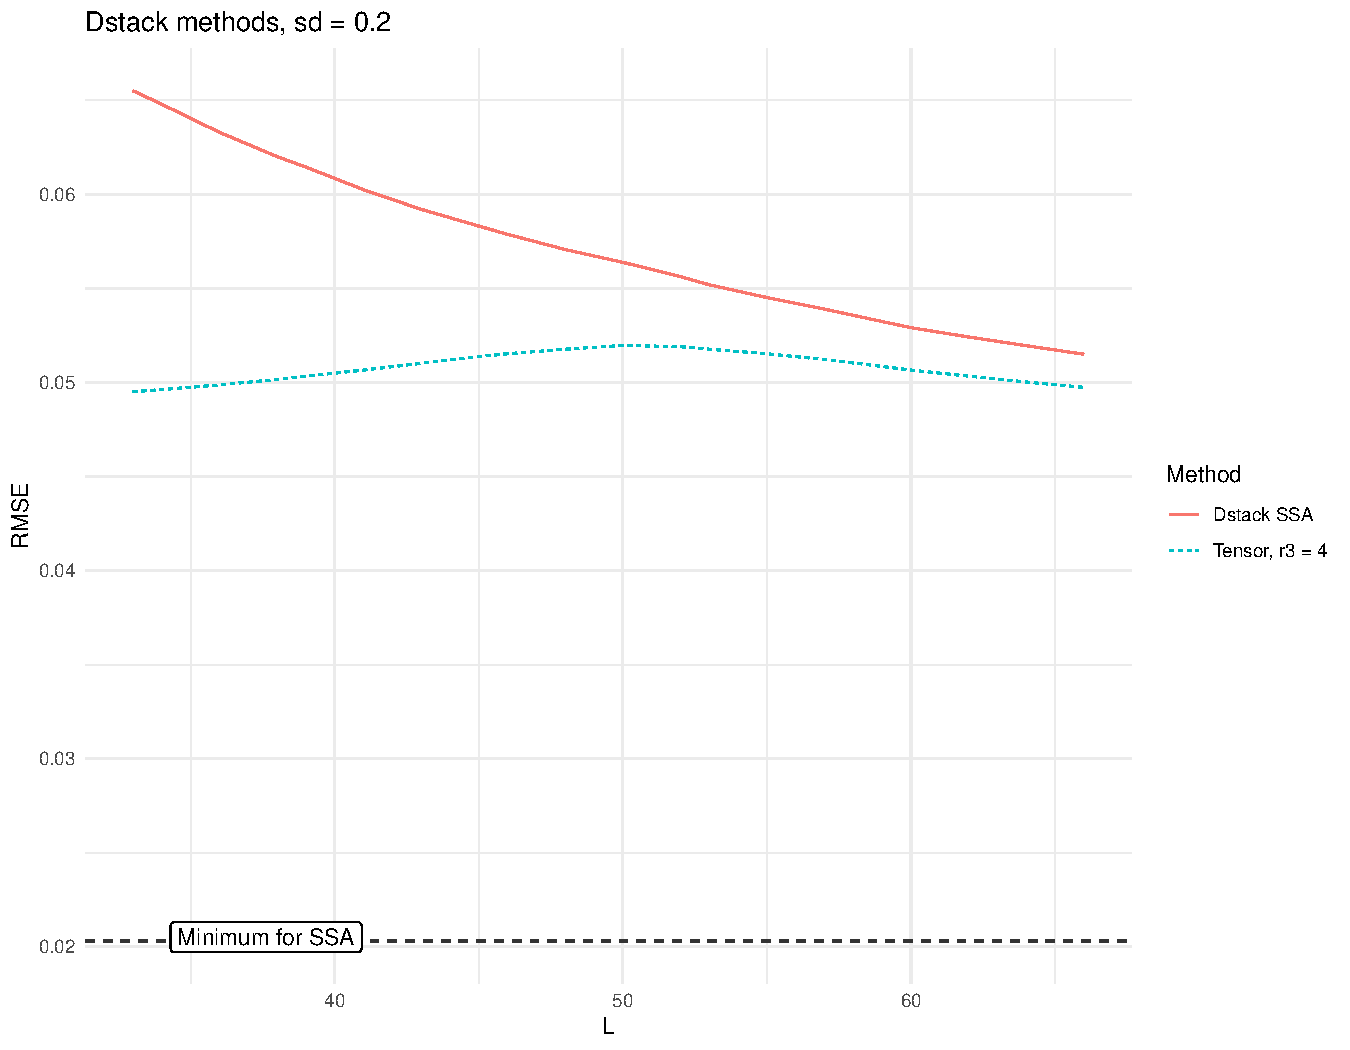
\includegraphics[width=\textwidth]{htlsd_byL_real_rec_rmse_dstack_2.pdf}
  \end{minipage}
  \caption{Зависимость RMSE оценки частот методами ESPRIT и
  модификациями Dstack от длины окна. Случай $\sigma = 0.2$.}
  \label{fig:dstack-ssa-byL-small}
\end{figure}
\begin{figure}
  \begin{minipage}{0.48\textwidth}
    \centering
    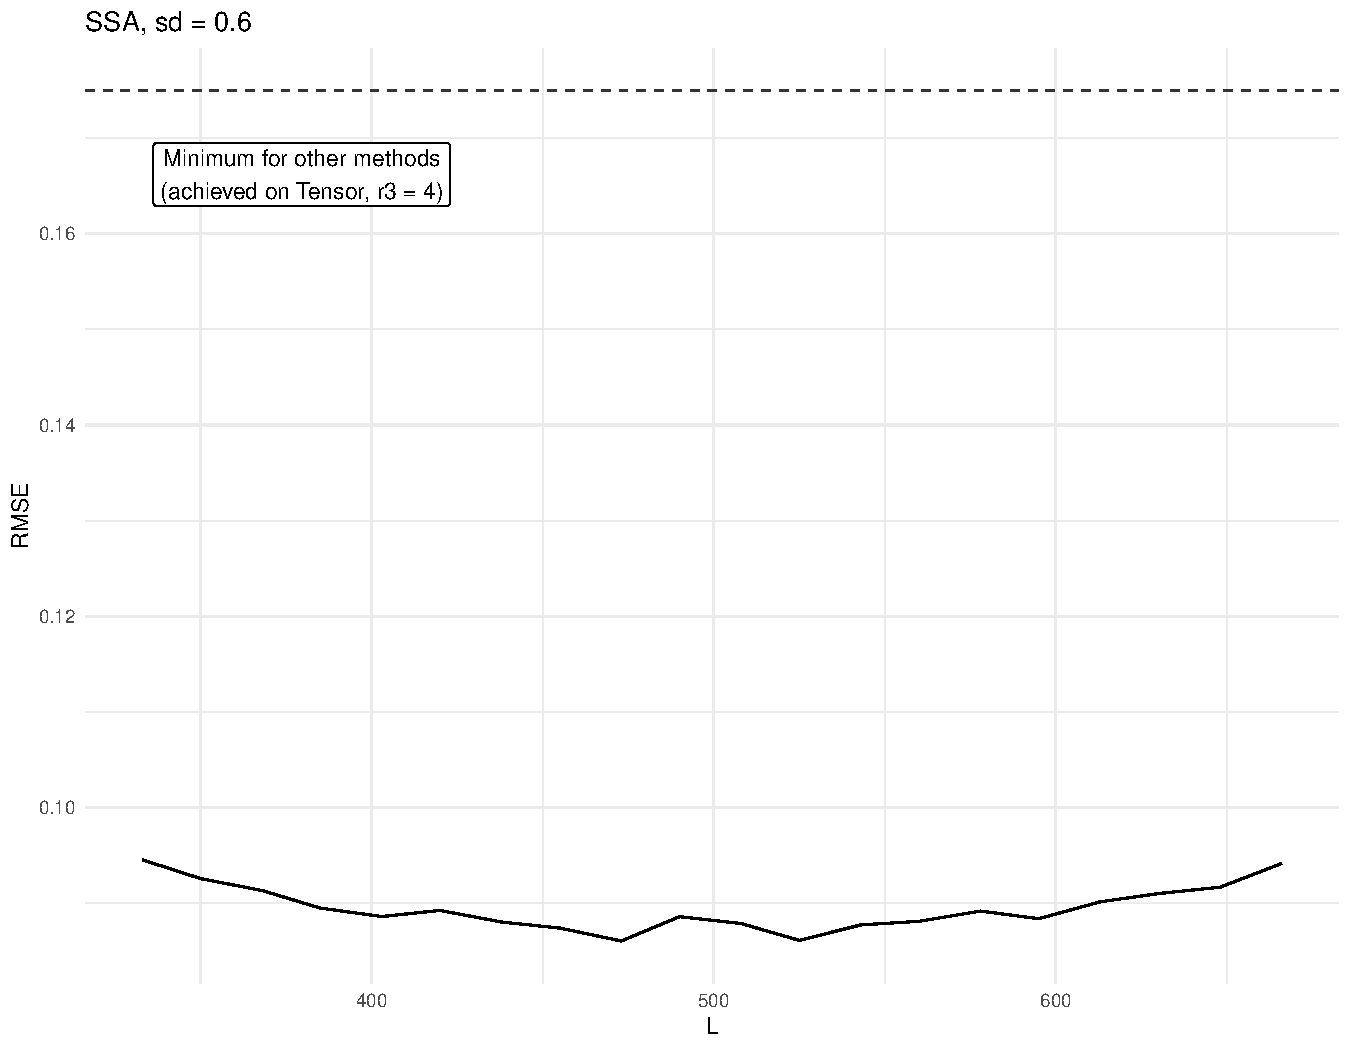
\includegraphics[width=\textwidth]{htlsd_byL_real_rec_rmse_ssa_3.pdf}
  \end{minipage}
  \begin{minipage}{0.48\textwidth}
    \centering
    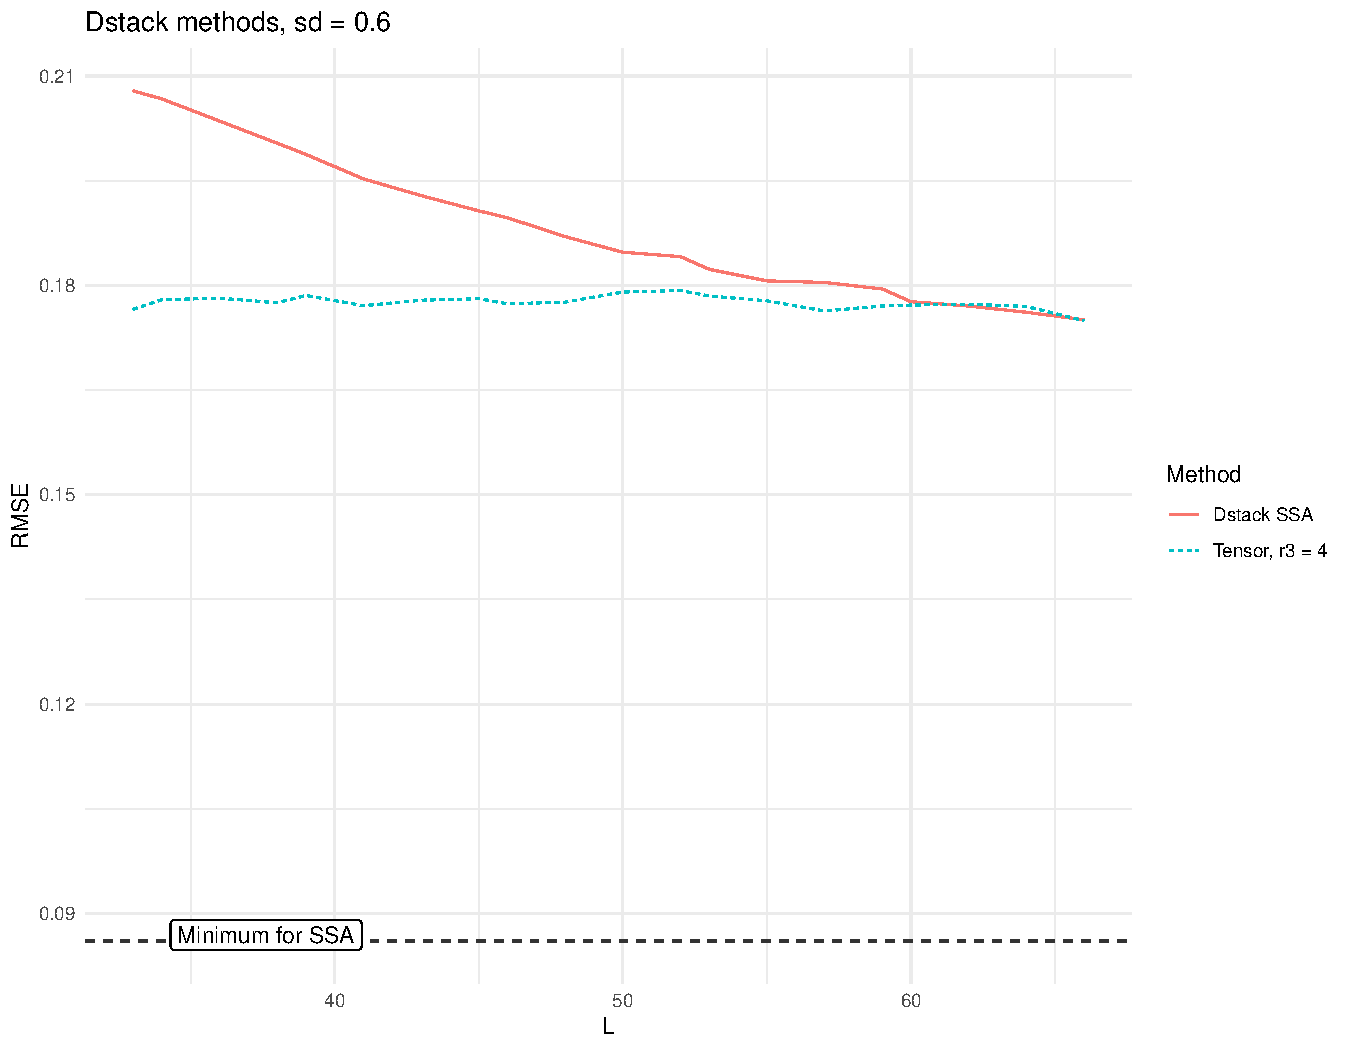
\includegraphics[width=\textwidth]{htlsd_byL_real_rec_rmse_dstack_3.pdf}
  \end{minipage}
  \caption{Зависимость RMSE оценки частот методами ESPRIT и
  модификациями Dstack от длины окна. Случай $\sigma = 0.6$.}
  \label{fig:dstack-ssa-byL-large}
\end{figure}

Из графиков видно, что при любом уровне шума SSA выделяет сигнал
значительно точнее, чем Dstack методы.
При выборе оптимальных длин окна методы Dstack SSA и Dstack HO-SSA
близки по точности, с небольшим преимуществом тензорного метода.

\section{Другие варианты применения тензорных разложений в задаче
выделения сигнала}\label{sec:review}
В данном разделе приведён краткий обзор статей, не рассмотренных
ранее, в которых предлагается использовать вложение ряда в тензор, и
последующее его тензорное разложение в задачах выделения сигнала или
оценки параметров.
Также описаны возможные перспективы дальнейшего изучения тензорных методов.

\subsection{Тензорный SSA с использованием {$(L_r, L_r, 1)$}-разложения}
\label{subsec:review-lrlr1}
В статье~\cite{DeLathauwer2011} рассматривается задача выделения
сигнала в многомерном ряде
\[
  \bfY = \bfM \bfS + \bfN,
\]
где $\bfY$ "--- наблюдаемый ряд, $\bfS$ "--- искомый сигнал, $\bfM$
"--- коэффициенты линейных комбинаций, с которыми сигнал составляет
наблюдаемый ряд, $\bfN$ "--- шум.
Траекторный тензор ряда определяется так же, как в
определении~\ref{def:traj-tensor-ssa}.
Приводится теоретическая информация про разложение в сумму тензоров с
$n$-рангами $(L_r, L_r, 1)$, которое называется $(L_r, L_r,
1)$-разложением, в частности приводятся определение и условия единственности.

Для модели, в которой сигнал составляют суммы произведений полиномов
и комплексных экспонент, доказаны условия единственности $(L_r, L_r,
1)$-разложения траекторного тензора ряда.

Сам метод заключается в построении траекторного тензора по ряду $\bfY$,
аппроксимации этого тензора меньшими $n$-рангами (но б\'{о}льшими, чем
$n$-ранги самого сигнала), и применении $(L_r, L_r, 1)$-разложения к
этой аппроксимации.
Далее по этому разложению строится оценка сигнала $\bfS$.

В работе проводятся численные сравнения точности выделения сигнала
предложенным методом при различных выборах параметров рангов
аппроксимации и $L_r$, однако сравнения с другими методами выделения
сигнала не проводятся.

В дальнейшем возможно провести численное сравнение предлагаемого
метода с SSA, MSSA и HO-MSSA с точки зрения точности выделения
сигнала и разделения компонент сигнала.

\subsection{Тензорный SSA с использованием CPD}
В работе~\cite{TSSA} рассматривается задача выделения одномерного
вещественного сигнала из ряда с нестационарным шумом.

Вводится понятие траекторного тензора следующим образом: исходный
одномерный ряд делится на непересекающиеся подряды длины $l$, затем
траекторный тензор строится аналогично траекторному тензору
многомерного ряда из определния~\ref{def:trajectory-tensor-mssa}, как
если бы эти подряды были каналами многомерного сигнала.
Предлагается алгоритм Tensor-Based SSA (TSSA), основанный на применении CPD
к полученному траекторному тензору ряда.

Кроме того, предлагается алгоритм TSSA-EMD, основанный на
использовании метода EMD~\cite{Lin2005} для адаптивной группировки
компонент CPD.
Метод заключается в получении CPD траекторного тензора, использовании
EMD для выделения сигнала, построении траекторного тензора $\calF$
этой оценки сигнала, и решении оптимизационных задач
\[
  J(\calG_{ijk}) = \left\|\calF_{ijk} - \sum_{r=1}^{R}\calG_{ijk}
  a_{ir} b_{jr}
  c_{kr}\right\|^2 \to \min_{\calG_{ijk}}
\]
для всех $i$, $j$, $k$, где $a_{ir}$, $b_{jr}$ и $c_{kr}$ "---
элементы компонент CPD.
После нахождения тензора адаптивных весов $\calG=\{\calG_{ijk}\}$
строится оценка
траекторного тензора сигнала
\[
  \calS_{ijk} = \sum_{r=1}^{R}\calG_{ijk} a_{ir} b_{jr} c_{kr},
\]
по которому восстанавливается оценка сигнала.

Метод TSSA-EMD численно сравнивался с SSA и другими методами
выделения сигнала на моделированном ряде с
нестационарным шумом, причём явная
формула рассматриваемого ряда в статье не приведена.
Было показано значимое преимущество TSSA-EMD над остальными
рассматриваемыми методами в смысле RMSE, причём для каждого алгоритма
рассматривался лишь один набор параметров.
Также было рассмотрено применение TSSA-EMD к реальному ряду.

Мной был рассмотрен метод с применением CPD, но без использования EMD
и тензора адаптивных весов, и численные сравнения показали значимое
преимущество
базового SSA над предлагаемым методом.
В дальнейшем имеет смысл рассмотреть предлагаемый метод с
использованием адаптивных весов с точки зрения точности выделения
сигнала, причём можно заменить EMD на другие методы выделения сигнала.

\subsection{Tensor SSA с использованием T-SVD}
В работе~\cite{TrungLe2024} рассматривается задача выделения
многомерного сигнала.
Траекторныый тензора сигнала строится аналогично
определению~\ref{def:trajectory-tensor-mssa}.
К тензору применяется разложение T-SVD~\cite{Kilmer2011,Kilmer2013}, которое
является разложением Таккера с $f$-диагональным ядром разложения, то
есть сечения 3-го направления этого тензора "--- диагональные матрицы.

В статье приводится утверждение о <<трубном>> (tubal) ранге траекторных
тензоров рядов, представимых в виде суммы произведений полиномов,
экспонент и гармоник.
Трубный ранг тензора "--- это число ненулевых векторов 3-го
направления в ядре разложения $\calZ$ этого тензора.
Также приводится утверждение о связи T-SVD с кратковременным
преобразованием Фурье.

Авторы приводят лишь визуальное сравнение с методом TenSOFO на
примере отделения
электрокардиограммы плода от электрокардиограммы матери, и не
приводят никаких метрик точности выделения сигнала.

Мной был рассмотрен предлагаемый метод, и были проведены численные
сравнения с методами MSSA и HO-MSSA на малом наборе рядов.
Предлагаемый метод оказался наименее точным.
В дальнейшем для полноты возможно провести сравнения на большем
классе сигналов.

\newpage

\section{Заключение}\label{sec:conclusion}
В результате работы было показано, что тензорные модификации
алгоритма \linebreak
ESPRIT в задаче оценки параметров одномерных и многомерных
комплексных сигналов при оптимальном выборе параметров
длин окна оказываются точнее стандартного метода ESPRIT,
что соотносится с результатами работы~\cite{hosvd-hooi-separation}.
Однако преимущество тензорных алгоритмов мало, и множество
длин окна, при которых это преимущество есть, также невелико.

Также в работе показано, что в отличие от задачи
оценки параметров, тензорные методы в задаче выделения комплексных
сигналов имеют преимущество лишь в случае многомерных сигналов.
Метод HO-SSA выделяет одномерные комплексные сигналы существенно менее точно,
чем базовый SSA, а метод HO-MSSA выделяет многомерные комплексные сигналы
точнее метода MSSA, хотя преимущество и не велико а трудоёмкость тензорного
метода больше, чем стандартного.
Это соотносится с результатами исследования методов HO-SSA и
HO-MSSA в задаче выделения вещественных сигналов.

С другой стороны, было показано, что при достаточно близких частотах
и высоком уровне шума стандартный методы ESPRIT может перестать
идентифицировать все параметры сигнала, в то время как использование
Dstack HO-ESPRIT в этих же условиях продолжает
оценивать параметры с высокой точностью.
Однако применение Dstack модификаций в задаче оценки параметров
затруднено необходимостью того, чтобы выполнялось некоторое
достаточно строгое условие на частоты, представленные в сигнале.
В задаче выделения сигнала, стандартный метод SSA оказался точнее
Dstack модификаций при любом уровне шума.

Кроме того, было показано, что точность выделения
одномерных сигналов методом HO-SSA можно увеличить, восстанавливая
сигнал усечением траекторного тензора лишь по части его направлений.
Однако этого увеличения точности всё ещё недостаточно, чтобы
тензорный метод был точнее стандартного SSA.

\bibliography{main}
\bibliographystyle{ugost2008}
\end{document}
